% \documentclass[review]{cvpr}
\documentclass[final]{cvpr}

\usepackage{mathptmx}
\usepackage{epsfig}
\usepackage{graphicx}
\usepackage{amsmath}
\usepackage{amssymb}
\usepackage{subfig}

% Include other packages here, before hyperref.

% If you comment hyperref and then uncomment it, you should delete
% egpaper.aux before re-running latex.  (Or just hit 'q' on the first latex
% run, let it finish, and you should be clear).
\usepackage[pagebackref=true,breaklinks=true,colorlinks,bookmarks=false]{hyperref}

\def\cvprPaperID{****} % *** Enter the CVPR Paper ID here
\def\confYear{CVPR 2021}
%\setcounter{page}{4321} % For final version only
\pdfminorversion=7

\begin{document}

%%%%%%%%% TITLE
\title{Automated Camera Stabilization and Calibration \\for Intelligent Transportation Systems}

\author{Marcel Bruckner\\
% Informatics 6 - Chair of Robotics, Artificial Intelligence and Real-time Systems\\
% TUM Department of Informatics\\
Technische Universität München\\
Boltzmannstraße 15, 85748 Garching\\
{\tt\small marcel.bruckner@tum.de}
}

\maketitle

% !TEX root=./report.tex

\newcommand{\Providentia}{\emph{\href{https://innovation-mobility.com/}{Providentia++}} project \cite{kraemmer2020providentia}} 
\newcommand{\TAADBW}{\emph{Test Area Autonomous Driving Baden-Württemberg} \cite{fleck2018towards}} 
\newcommand{\ITS}{Intelligent Transportation System}
\newcommand{\AD}{Autonomous Driving}
\newcommand{\HDmaps}{HD maps~(\ref{sec:hd_maps})}
\newcommand{\Sc}{static scene (\ref{sec:dynamic_foreground_static_scene})}
\newcommand{\DigitalTwin}{Digital~Twin~(\ref{sec:digital_twin})}
\newcommand{\OD}{OpenDRIVE}

\newcommand{\camsn}[1]{S{#1}0 Near}
\newcommand{\camsf}[1]{S{#1}0 Far}

\newcommand{\hr}{\noindent\rule{\linewidth}{0.4pt}}


\providecommand{\keywords}[1]
{
  \small	
  \textbf{\textit{Keywords---}} #1
}

\newcommand\blankpage{%
    \null
    \thispagestyle{empty}%
    \addtocounter{page}{-1}%
    \newpage}

%%%%%%%%% ABSTRACT
%!TEX root = ../report.tex
\begin{abstract}

In the emerging field of Intelligent Transportation Systems one main challenge is the fusion of different sensor types.
To fuse the measurements correctly each sensor needs to be free from noise and calibrated accurately.

In this work we focus on two problems resulting from environmental influences on RGB cameras within the Providentia++~project.

First we propose an online vision-based framework to remove jitter from shaky camera streams to dynamically stabilize the video feed.
We show that our approach based on visual features and an image space homographic transformation gives good stabilization results regarding the optical flow in the image. 
By exemplary tracking objects and measuring their travelled pixel distance we show a substantial decrease of the jittery image motion. 

Second we propose an online Bundle Adjustment formulation based on the reprojection-error to statically calibrate RBG-only cameras \wrt{} a high definition map and to mitigate drift of the intrinsic and extrinsic camera parameters over time.
By relaxing the minimization problem using a 1D-approximation of road signs we achieve high accuracy in the calibration of the cameras.
We show the minimal number of needed correspondences between the video stream and the map, the structure they have to exceed and give a lower bound on the remaining calibration error. 

\end{abstract}


\keywords{
    Intelligent Transportation Systems,
    Computer Vision,
    Video Stabilization,
    Feature Detection,
    Feature Matching,
    Camera Calibration,
    Bundle Adjustment,
    Reprojection-error,
    Optimization,
    OpenDRIVE
}


%%%%%%%%% BODY TEXT
% !TEX root=./report.tex

\section{Introduction}

Within the \Providentia{}, a section of the highway A9 between Munich and Nuremberg was converted to a testing site for autonomous driving. 
As part of this, a large sensor network system has been set up along the highway to allow monitoring and steering of traffic as well as to improve the coordination between autonomous and traditional cars. 
The primary task of the intelligent transportation system (ITS) is to create a digital traffic twin that accurately represents the physical road situation in real-time. 
Based on this digital twin, the smart infrastructure can provide a far-reaching and comprehensive view to the drivers and autonomous cars in order to improve their situational awareness within the current traffic environment.

A key challenge of ITS lies in the reliable and accurate calibration of the different sensors.
The calibration is especially challenging when the sensor is subject to real-life disturbances like vibration of its mounting pole caused by wind or displacements due to temperature expansion.
In this work we focus on removing the noise introduced by the disturbances and its implications for the vision system built upon the cameras mounted to gantry bridges.

We propose two computer vision based approaches to tackle the real-life disturbances and to remove noise from the system.
The solved problems can be roughly grouped into problems concerning the dynamic stabilization of the video feed and the static calibration of the camera setup.

\paragraph{Dynamic Stabilization}
The cameras are constantly exposed to wind and vibrations from passing vehicles.
These influences propagate into the video stream and result in jittery motion of the images.
We propose a pipeline to counteract the shaky motions of the cameras using a digital image stabilization approach.
The approach is based on visual image features that are matched between the current and a stable reference frame. 
The feature matching is used to minimize the reprojection-error between the frames and results in a homographic transformation.
We use the transformation to align the static backgrounds of the frames, thus mitigating the real-world motions of the camera in the image space.

\paragraph{Static Calibration}
We track and predict the real world location of the vehicles in the test to pass this information to the drivers and autonomous vehicles. 
To accurately predict the locations the system needs to be calibrated precisely towards a global reference frame. 
This is a time consuming process that often has to be done by hand. 
The cameras translational, rotational and intrinsic parameters decalibrate over time due to environmental influences on the mounting constructions and gantry bridges as well as from the natural wear of the materials.

Within the project high definition maps (HD maps) of the enclosed environment are used extensively. 
These HD maps offer the approximations of the real-world positions of the highway lanes, the gantry bridges, objects like poles and permanent delineators and traffic signals like speed limits or exit markers.
We use this spatial information and a mapping from the objects to pixels in the video frame to solve a Bundle Adjustment (BA) problem by minimizing the reprojection-error.
We jointly optimize for the cameras intrinsic and extrinsic parameters as well as the real-world locations to recover the camera poses form the observations.

\paragraph{Code Repositories}
The code for the dynamic stabilization, static calibration and object position retrieval from the HD maps are accessible via two GitHub repositories: \url{https://github.com/Brucknem/GuidedResearch} and \url{https://github.com/Brucknem/OpenDRIVE}.

% % !TEX root=./report.tex

\section{Terms and Definitions}
This section provides explanations of extensively used terms and definitions. 

\subsection{Digital Twin}
\label{sec:digital_twin}

\subsection{Dynamic foreground and static scene}
\label{sec:dynamic_foreground_static_scene}
We group parts of the world seen by the cameras into the two groups of dynamic foreground and static scene.
Dynamic foreground describes all pixels that represent objects that are meant to be moving, \eg{} vehicles on the roads.
On the other hand the static scene are all pixels that are not dynamic foreground, \eg{} the road, guardrails or bridges.

\subsection{Parametric cubic polynomial}
To calculate a parametric cubic polynomial the following equation is used.
\begin{equation}
    \begin{split}
        para(U, s) &= para(U_a, U_b, U_c, U_d, s) \\ &= U_a + U_b * s + U_c * s^2 + U_d * s^3
    \end{split}
\end{equation}
\section{Related Work}
There are many ITS projects emerging recently  \cite{koster2017testfeld,arnold2020cooperative,arnoldCooperativePerception,agrawal2008censure}. 
They propose novel approaches to the detection, tracking and traffic prediction problems that arise with the goal to provide additional environment information to human drivers and autonomous vehicles.
Erdelean \etal{} \cite{erdelean2019catalogue} give a detailed overview over the existing projects up to the year 2019.

In the \TAADBW{} (TAADBW) project multiple optical camera sensors are attached to large poles with overlapping fields of view.
They calibrate their cameras relative to a high-precision map and assume the calibration and the intrinsic camera parameters to be static during runtime. 
The team relies on a manual a-priori selection of visual landmarks and perform calibration at system startup.  
The team of the TAADBW estimate the extrinsic calibration with exact world position from the map by minimizing the squared distances between the visible landmarks and the respective projected objects.
The large overlaps in the fields of view in their setup allow a global optimization strategy. 
This is not feasible in our project due to the small overlaps in the fields of view between the cameras \cite{kraemmer2020providentia} and associating pixels within the multi-view setup is an inherently hard problem. 

Müller \etal{} \cite{laciMueller} present an approach based on a cooperative intelligent vehicle.
The vehicle moves through the scene and passes cooperative awareness messages containing positional information from the vehicle to the infrastructure. 
This removes the need for overlapping fields of view completely and enables a fully automated and sensor-independent registration.
The team calibrates a multitude of different sensor types to the world frame and recovers their extrinsic parameters. 

Calibration between cameras and radar sensors has been solved previously by Schöller \etal{} within the \Providentia{}.

An overview over the general structure of Bundle Adjustment problems as used in \autoref{sec:static_calibration_approach} is given by Triggs \etal{} in \cite{triggs10.1007/3-540-44480-7_21}.
% None of the teams - to the best of our knowledge - provide in depth public information about their camera stabilization and calibration approaches.
% !TEX root=./report.tex

\section{Approach}
In this paper we propose two algorithms to solve distinct problems that arise from real-world disturbances that act upon the ITS.

\subsection{Dynamic Stabilization}
\label{sec:dynamic_stabilization_approach}

\begin{figure}[t]
   \begin{center}
      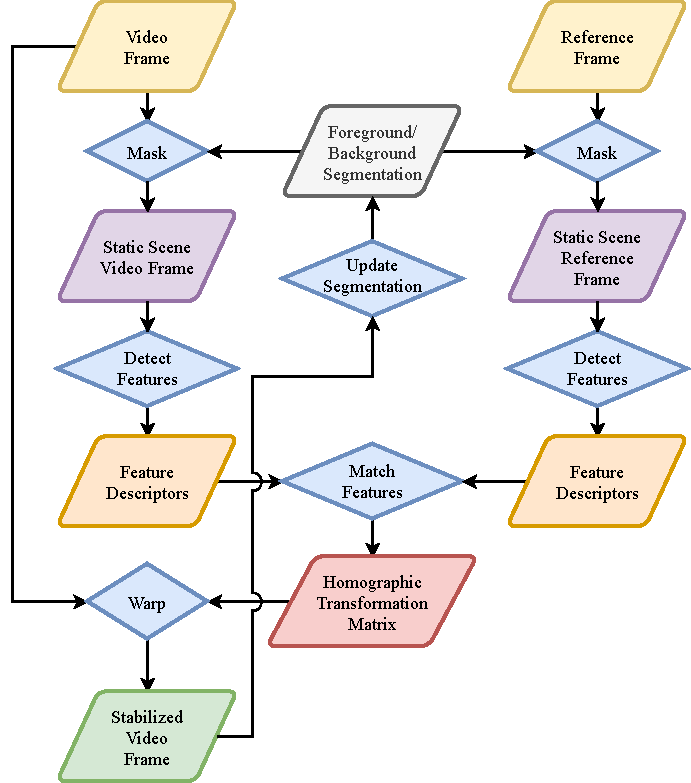
\includegraphics[width=0.8\linewidth]{diagrams/DynamicStabilization.pdf}
   \end{center}
   \caption{
      The proposed dynamic stabilization pipeline. 
      The input is the video and a stable reference frame.
      The frames are segmented into the foreground and background to extract the static scene.
      On the static scene visual features are detected and the feature descriptors are matched.
      We use the homographic transformation minimizing the reprojection-error based on the matching to warp the video frame.
      The stabilized frame is used to update the background segmentation mask.
       }
   \label{fig:dynamic_stabilization_algorithm}
\end{figure}

The camera sensors used in the project are mounted to gantry bridges spanning over the highway.
Environmental influences, \eg{} wind or vibrations from passing vehicles, bring the bridges into a swinging state that spreads onto the cameras. 
This unwanted real world movement propagates into the video feeds output by the camera and introduces jittery motion in image space. 
We assume the cameras to be mostly static, thus we only face disturbances within a small range around the resting position.
Nonetheless, the small disturbances get amplified by the huge distances covered by the cameras and introduce substantial error.

To mitigate the noise added by the jittery motion we propose the pipeline displayed in \autoref{fig:dynamic_stabilization_algorithm} and explained in the following.

%%%%%%%%%%%%%%%%%%%%%%%%%%%%%%%%%%%%%%%%%%%%%%%%%%%%%%%%%%%%%%%%%%%%%%%%%%%%%%%%%%%%%%%%%%%%%%%%%%%%%%%%%%%%%%%%%%%%
%%%%%%%%%%%%%%%%%%%%%%%%%%%%%%%%%%%%%%%%%%%%%%%%%%%%%%%%%%%%%%%%%%%%%%%%%%%%%%%%%%%%%%%%%%%%%%%%%%%%%%%%%%%%%%%%%%%%
%%%%%%%%%%%%%%%%%%%%%%%%%%%%%%%%%%%%%%%%%%%%%%%%%%%%%%%%%%%%%%%%%%%%%%%%%%%%%%%%%%%%%%%%%%%%%%%%%%%%%%%%%%%%%%%%%%%%

\paragraph{Extract the Static Background}
We stabilize the input frame by minimizing the reprojection-error between the video frame and the reference frame, thus aligning the images.
This alignment is based on the matching of features between the frames, whereas we do not align the moving vehicles, but only the static non-moving background, \eg{} the road, poles, guardrails and bridges.
We assume that the background does not move in the real world, thus aligning it during image warping ensures that the scene stays static and only the vehicles real movement is kept.
Hence, we extract the static background from the input frame and the stable reference frame using a background segmentation based on
the \emph{Improved Adaptive Gaussian Mixture Model for Background Subtraction} proposed by Zoran Zivkovic \etal{} \cite{zivkovic10.5555/1018428.1020644,zivkovic10.1016/j.patrec.2005.11.005,opencv_library}.

%%%%%%%%%%%%%%%%%%%%%%%%%%%%%%%%%%%%%%%%%%%%%%%%%%%%%%%%%%%%%%%%%%%%%%%%%%%%%%%%%%%%%%%%%%%%%%%%%%%%%%%%%%%%%%%%%%%%
%%%%%%%%%%%%%%%%%%%%%%%%%%%%%%%%%%%%%%%%%%%%%%%%%%%%%%%%%%%%%%%%%%%%%%%%%%%%%%%%%%%%%%%%%%%%%%%%%%%%%%%%%%%%%%%%%%%%
%%%%%%%%%%%%%%%%%%%%%%%%%%%%%%%%%%%%%%%%%%%%%%%%%%%%%%%%%%%%%%%%%%%%%%%%%%%%%%%%%%%%%%%%%%%%%%%%%%%%%%%%%%%%%%%%%%%%

\paragraph{Feature Detection}
\begin{figure}[t]
   \begin{center}
      \includegraphics[width=\linewidth]{images/feature_matching.png}
   \end{center}
   \caption{
      Left: The input frame. 
      Right: The stable reference frame.
      The colorful lines display the matching between image features. 
      The ends of the lines are the location of the features.
       }
   \label{fig:dynamic_stabilization_feature_matching}
\end{figure}

We search the static background for pixel locations that are prominent and depict specific patterns that are unique and can easily be compared.
The detected features describe the location based on different metrics, \eg{} the local image gradient, oriented histograms or haar-like features \cite{stork2001pattern}.
Kumar \etal{} \cite{kumar2014survey} give an in depth description of a multitude of feature detectors and descriptors.

We implemented the SURF \cite{bay10.1007/11744023_32} and ORB \cite{rublee6126544} feature detectors and descriptors and the Fast \cite{Ghahremani_2021} feature detector with FREAK \cite{alahi6247715} feature descriptors. The algorithmic implementation is taken from the OpenCV library \cite{opencv_library}. 

%%%%%%%%%%%%%%%%%%%%%%%%%%%%%%%%%%%%%%%%%%%%%%%%%%%%%%%%%%%%%%%%%%%%%%%%%%%%%%%%%%%%%%%%%%%%%%%%%%%%%%%%%%%%%%%%%%%%
%%%%%%%%%%%%%%%%%%%%%%%%%%%%%%%%%%%%%%%%%%%%%%%%%%%%%%%%%%%%%%%%%%%%%%%%%%%%%%%%%%%%%%%%%%%%%%%%%%%%%%%%%%%%%%%%%%%%
%%%%%%%%%%%%%%%%%%%%%%%%%%%%%%%%%%%%%%%%%%%%%%%%%%%%%%%%%%%%%%%%%%%%%%%%%%%%%%%%%%%%%%%%%%%%%%%%%%%%%%%%%%%%%%%%%%%%

\paragraph{Feature Matching}
We compare the detected features from the input frame with the features from the stable reference frame.
A match is reported if the feature descriptors of two compared features surpass the Lowe's ratio test \cite{lowe10.1023/B:VISI.0000029664.99615.94} regarding some feature dependent metric \cite{kumar2014survey}.
These feature matches establish a spatial relationship in pixel space between the two frames.
\autoref{fig:dynamic_stabilization_feature_matching} displays an exemplary feature matching.

We estimate a homographic transformation $H$ that maps the homogeneous pixel locations $(x_i, y_i, 1)^T$ of the input frame to the matched pixel locations $(x'_i, y'_i, 1)^T$ in the stable reference frame.
We minimize the reprojection-error between the pixels so that for each match $i$ it holds
\begin{equation}
 z_i  * (x'_i, y'_i, 1)^T \sim H * (x_i, y_i, 1)^T
 \label{eq:dynamic_stabilization_homographic_transformation}
\end{equation}
where $z_i$ is the homogeneous component used in the perspective division. 
We use a RANSAC \cite{fischler1981random} based estimation procedure to robustify the minimization against outliers.

The algorithmic implementation is included in the OpenCV library \cite{opencv_library}.

%%%%%%%%%%%%%%%%%%%%%%%%%%%%%%%%%%%%%%%%%%%%%%%%%%%%%%%%%%%%%%%%%%%%%%%%%%%%%%%%%%%%%%%%%%%%%%%%%%%%%%%%%%%%%%%%%%%%
%%%%%%%%%%%%%%%%%%%%%%%%%%%%%%%%%%%%%%%%%%%%%%%%%%%%%%%%%%%%%%%%%%%%%%%%%%%%%%%%%%%%%%%%%%%%%%%%%%%%%%%%%%%%%%%%%%%%
%%%%%%%%%%%%%%%%%%%%%%%%%%%%%%%%%%%%%%%%%%%%%%%%%%%%%%%%%%%%%%%%%%%%%%%%%%%%%%%%%%%%%%%%%%%%%%%%%%%%%%%%%%%%%%%%%%%%

\paragraph{Image Alignment}
We use the found homographic transformation to warp the whole input frame, thus aligning the background of the frames.
As the keyframe is stable and does not change over time the current video frame is also stabilized.
The alignment minimizes the motion of the static background scene and leaves only the real expected movement of the vehicles.

%%%%%%%%%%%%%%%%%%%%%%%%%%%%%%%%%%%%%%%%%%%%%%%%%%%%%%%%%%%%%%%%%%%%%%%%%%%%%%%%%%%%%%%%%%%%%%%%%%%%%%%%%%%%%%%%%%%%
%%%%%%%%%%%%%%%%%%%%%%%%%%%%%%%%%%%%%%%%%%%%%%%%%%%%%%%%%%%%%%%%%%%%%%%%%%%%%%%%%%%%%%%%%%%%%%%%%%%%%%%%%%%%%%%%%%%%
%%%%%%%%%%%%%%%%%%%%%%%%%%%%%%%%%%%%%%%%%%%%%%%%%%%%%%%%%%%%%%%%%%%%%%%%%%%%%%%%%%%%%%%%%%%%%%%%%%%%%%%%%%%%%%%%%%%%

\paragraph{Foreground/Background Segmentation Upate}
We use the stabilized frame to update the segmentation of the foreground and background.
We assume the motion between frames to be relatively small, thus we use the segmentation of the stabilized frame for the next frame.
This reduces the search space for the feature detectors and prohibits matches between static scene and dynamic foreground objects. 
% Hence, the algorithm is robustified and speed up.

% !TEX root=./report.tex

\subsection{Static calibration}

\ITS{} are inherently dependent on the calibration of the different sensors. 
To track and predict traffic the system has to know the poses of the different sensors relative to some reference coordinate system.
This enables the ITS to accurately measure the position of vehicles within the single sensor ranges and at the overlapping boundaries.

Previous experiments have shown that a calibration process based on an IMU is not feasible in our case. 
Instead we focus on a calibration procedure based on visual landmarks in the video feed.
The landmarks are mapped to their partially known world positions from high definition road maps. 

%%%%%%%%%%%%%%%%%%%%%%%%%%%%%%%%%%%%%%%%%%%%%%%%%%%%%%%%%%%%%%%%%%%%%%%%%%%%%%%%%%%%%%%%%%%%%%%%%%%%%%%%%%%%%%%%%%%%%%%%%%%%%%%%%%%%%%%%%%%%%%%%%%%%%%%%%%%%%%%%%

\paragraph{Retrive objects from the \HDmaps}
In this work we focus on the permanent delineator objects that are easily visible in the video feeds.

The world position of the objects can be retrieved using the mathematical operations defined in the \OD{} standard.

This gives us the the base origin point $o~=~(x, y, z)^T$ of the object in the transverse mercator projection \cite{proj}. 
The base origin point is the world position of the lower end of the object where it ends in the ground or another object.

Additionally we retrieve a directional heading axis $d~=~(x, y, z)^T$ and the height $h$ of the object.

These values enable us to approximate the real-world objects by sampling points $s \in S$ in world position along the center line of the object, where 
\begin{equation}
S = \{s | s = o + \lambda * d: \quad \lambda \in [0, h]\}
\end{equation}
%%%%%%%%%%%%%%%%%%%%%%%%%%%%%%%%%%%%%%%%%%%%%%%%%%%%%%%%%%%%%%%%%%%%%%%%%%%%%%%%%%%%%%%%%%%%%%%%%%%%%%%%%%%%%%%%%%%%%%%%%%%%%%%%%%%%%%%%%%%%%%%%%%%%%%%%%%%%%%%%%

\paragraph{Mapping objects to pixels}

To calibrate the camera we need to establish a mapping
\begin{equation}
  s_c \mapsto p_c \Leftrightarrow  {o_c, d_c, \lambda_c} \mapsto p_c
\end{equation}
from pixels $p_c~=~(u,v)^T \in P$ from the video stream to the corresponding sampled points $s_c$ from the object they belong to.

This leaves us with a set $C$ of correspondences $\{p_c,s_c\}$.

This mapping is currently done by human interaction and not fully automated. 
To minimize the work an aiding system to mark pixels was implemented that outputs a list of pixels that can easily be mapped to the list of objects.

\begin{figure}[t]
  \begin{center}
  % \fbox{\rule{0pt}{2in} \rule{0.9\linewidth}{0pt}}
     \includegraphics[width=\linewidth]{images/hd_map_mapping.png}
  \end{center}
     \caption{Left: The current camera frame. Right: A part of the \HDmaps{}. Cyan: The mapping $s_c \mapsto p_c$ from objects (right) to their corresponding pixels (left).}
  \label{fig:hd_map_mapping}
  \end{figure}

%%%%%%%%%%%%%%%%%%%%%%%%%%%%%%%%%%%%%%%%%%%%%%%%%%%%%%%%%%%%%%%%%%%%%%%%%%%%%%%%%%%%%%%%%%%%%%%%%%%%%%%%%%%%%%%%%%%%%%%%%%%%%%%%%%%%%%%%%%%%%%%%%%%%%%%%%%%%%%%%%

\paragraph{Relaxation of problem by line approximation}
\begin{figure*}[!ht]
  \centering
  \begin{tabular}{cc}
    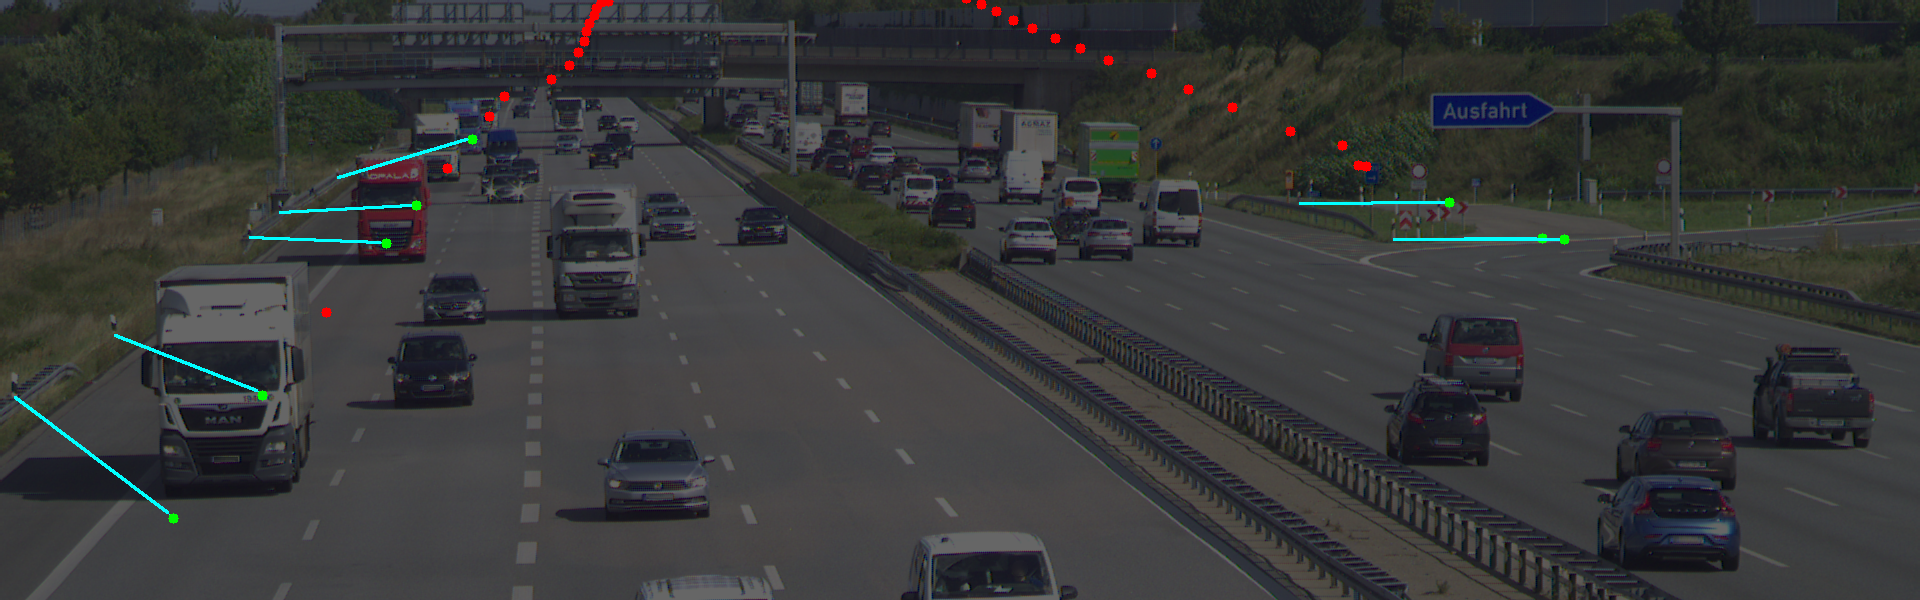
\includegraphics[width=0.4\linewidth]{images/calibration/background_uncalibrated_with_mapping.png}    &  
    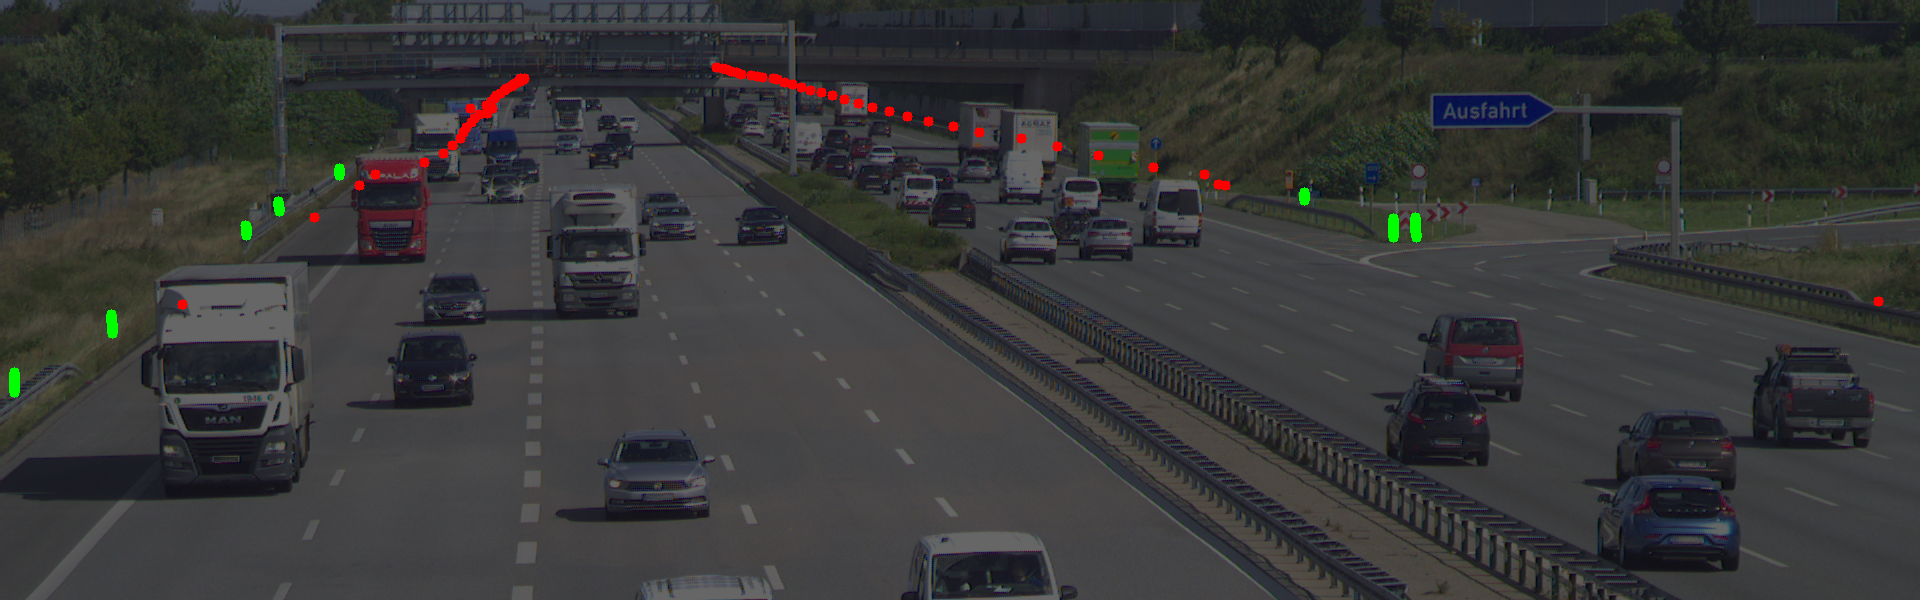
\includegraphics[width=0.4\linewidth]{images/calibration/background_calibrated.png}    
  \end{tabular}
  \caption{Left: Sampled points of objects that are mapped to pixel locations (green) and sampled points without known corresponding pixels (red) rendered by a poorly calibrated camera model.
  The mapping from the points to their expected pixels is drawn in cyan.
  Right: The same sampled points after the calibration procedure.
  The rendered positions of the sampled points align with the pixels of the objects they are mapped to and the drawn mapping disappears as the distance approaches $0$.  }
  \label{fig:calibration}
  \end{figure*}
Approximating the objects by lines removes the need for exactly known 3D correspondences as usually needed in calibration problems. 
Nonetheless it does not require to jointly estimate the full world position of the objects and camera pose jointly as in Bundle-Adjustment problems.
%
The assumptions we made are: 
\begin{itemize}
  \item Objects are symmetric around their directional heading axis.
  \item Pixels of the objects are also symmetric around the projected directional axis.
  \item The pixels in the mapping is equally distributed around the directional axis as the deviations from tangential offset points cancel out then. 
\end{itemize}

This models that the objects collapse into their center line in 2D and 3D and that tangentially deviating points on the surface in one direction equally cancels out by the opposite point mirrored at the center line.

%%%%%%%%%%%%%%%%%%%%%%%%%%%%%%%%%%%%%%%%%%%%%%%%%%%%%%%%%%%%%%%%%%%%%%%%%%%%%%%%%%%%%%%%%%%%%%%%%%%%%%%%%%%%%%%%%%%%%%%%%%%%%%%%%%%%%%%%%%%%%%%%%%%%%%%%%%%%%%%%%

\paragraph{Calibration procedure}
  
Our camera is modelled using the pinhole camera model. 
This uses the known intrinsic camera parameters and their corresponding projection $\pi$ from camera to image space.

The extrinsic camera parameters that map from world space to camera space are defined by the camera translation $T$ and the camera rotation $R$.
The translation and rotation are unknown, for them we optimize. 

We estimate the camera pose by minimizing a modified version of the reprojection error 
\begin{equation}
  \min_{T, R, \Lambda, W} E(P, S, T, R, \Lambda, W) 
\end{equation}
formulated as
\begin{equation}
  \begin{split}
    s_c =& o_c + \lambda_c * h_c \\
  E(P, S, T, R, \Lambda, W ) =& 
  \sum_{c \in C} 
  \left\lVert 
    w_c * [ p_c - \pi(T * R * s_c) ]
  \right\rVert_2^2 \\ 
  +& 
  \sum_{c \in C} 
  \left\lVert 
  penalize(\lambda_i, h_i)
  \right\rVert_2^2 \\ 
  +& 
  \sum_{c \in C} 
  \left\lVert 
  \alpha * (1 - w_i)
  \right\rVert_2^2 
\end{split}
\label{eq:reprojection_error}
\end{equation}
where $P$ is the set of mapped pixels in the image, $S$ is the set of mapped corresponding sampled points from the objects and $\Lambda$ is the set of $\lambda$ values associated with the sampled points.
This formulation allows the optimization over the line approximations of the objects and jointly optimizes for the camera parameters $T, R$ and the $\lambda \in \Lambda$ parameters of the line objects.

The calculation of the exact position of $s_c \sim \lambda$ allows the optimizer to search the whole space of real numbers for $\lambda$.
Nonetheless we penalize values for $\lambda$ that exceed the physical height of the object by 
\begin{equation}
    penalize(\lambda, h) =
    \begin{cases}
      \lambda - h,& \text{if } \lambda > h\\
      \lambda,    & \text{if } \lambda < 0\\
      0,    & \text{else}
    \end{cases} 
\end{equation}
This regularization enables a robust estimation procedure that can flexibly adjust to the missing exact world positions.

\paragraph{Initialization}
In contrast to most pose estimation problems our approach drops the need for good initialization. 
By regularization of the $\lambda$ values enough flexibility is given to optimize over an infinite space of values, 
but enforces the solution of the $\lambda$ to lie within the interval of $\lambda \in [0, h]$.

\begin{equation}
  \bar{s} = \frac{1}{\left\lvert C \right\rvert } \sum_{c \in C} o_c 
\end{equation}

\begin{equation}
  T_0 = \begin{pmatrix}
    1, 0, 0,& \bar{s}_x \\   
    0, 1, 0,& \bar{s}_y \\   
    0, 0, 1,& \bar{s}_z + 1000 \\   
    0, 0, 0,& 1   
  \end{pmatrix}
\end{equation}

\begin{equation}
  R_0 = \mathbb{I} ^ {4 \times 4}
\end{equation}

It is sufficient to initialize with $\lambda_c = 0$ for all correspondences.
The camera rotation is defined to be zero with the camera facing in negative world $z$ axis.
By placing the camera at some distance over the mean of the known object positions with zero rotation the optimization always converges to the desired minimum.

% \begin{itemize}
%   \item HD map based approach
%   \item Optimization algorithm, reprojection error between map and video 
%   \item Landmark extraction, mapping, pose estimation
%   \item Watersheder for pixel marking
%  translation can be  and initializing the camera at the some distance over the mean    
 % \end{itemize}
% !TEX root=./report.tex

\section{Evaluation}

We assure the correctness and quantify the visual improvements resulting from the algorithms by an empirical study on the video streams of the highway cameras.

\subsection{Study objects}
\begin{figure}[t]
    \begin{center}
    % \fbox{\rule{0pt}{2in} \rule{0.9\linewidth}{0pt}}
       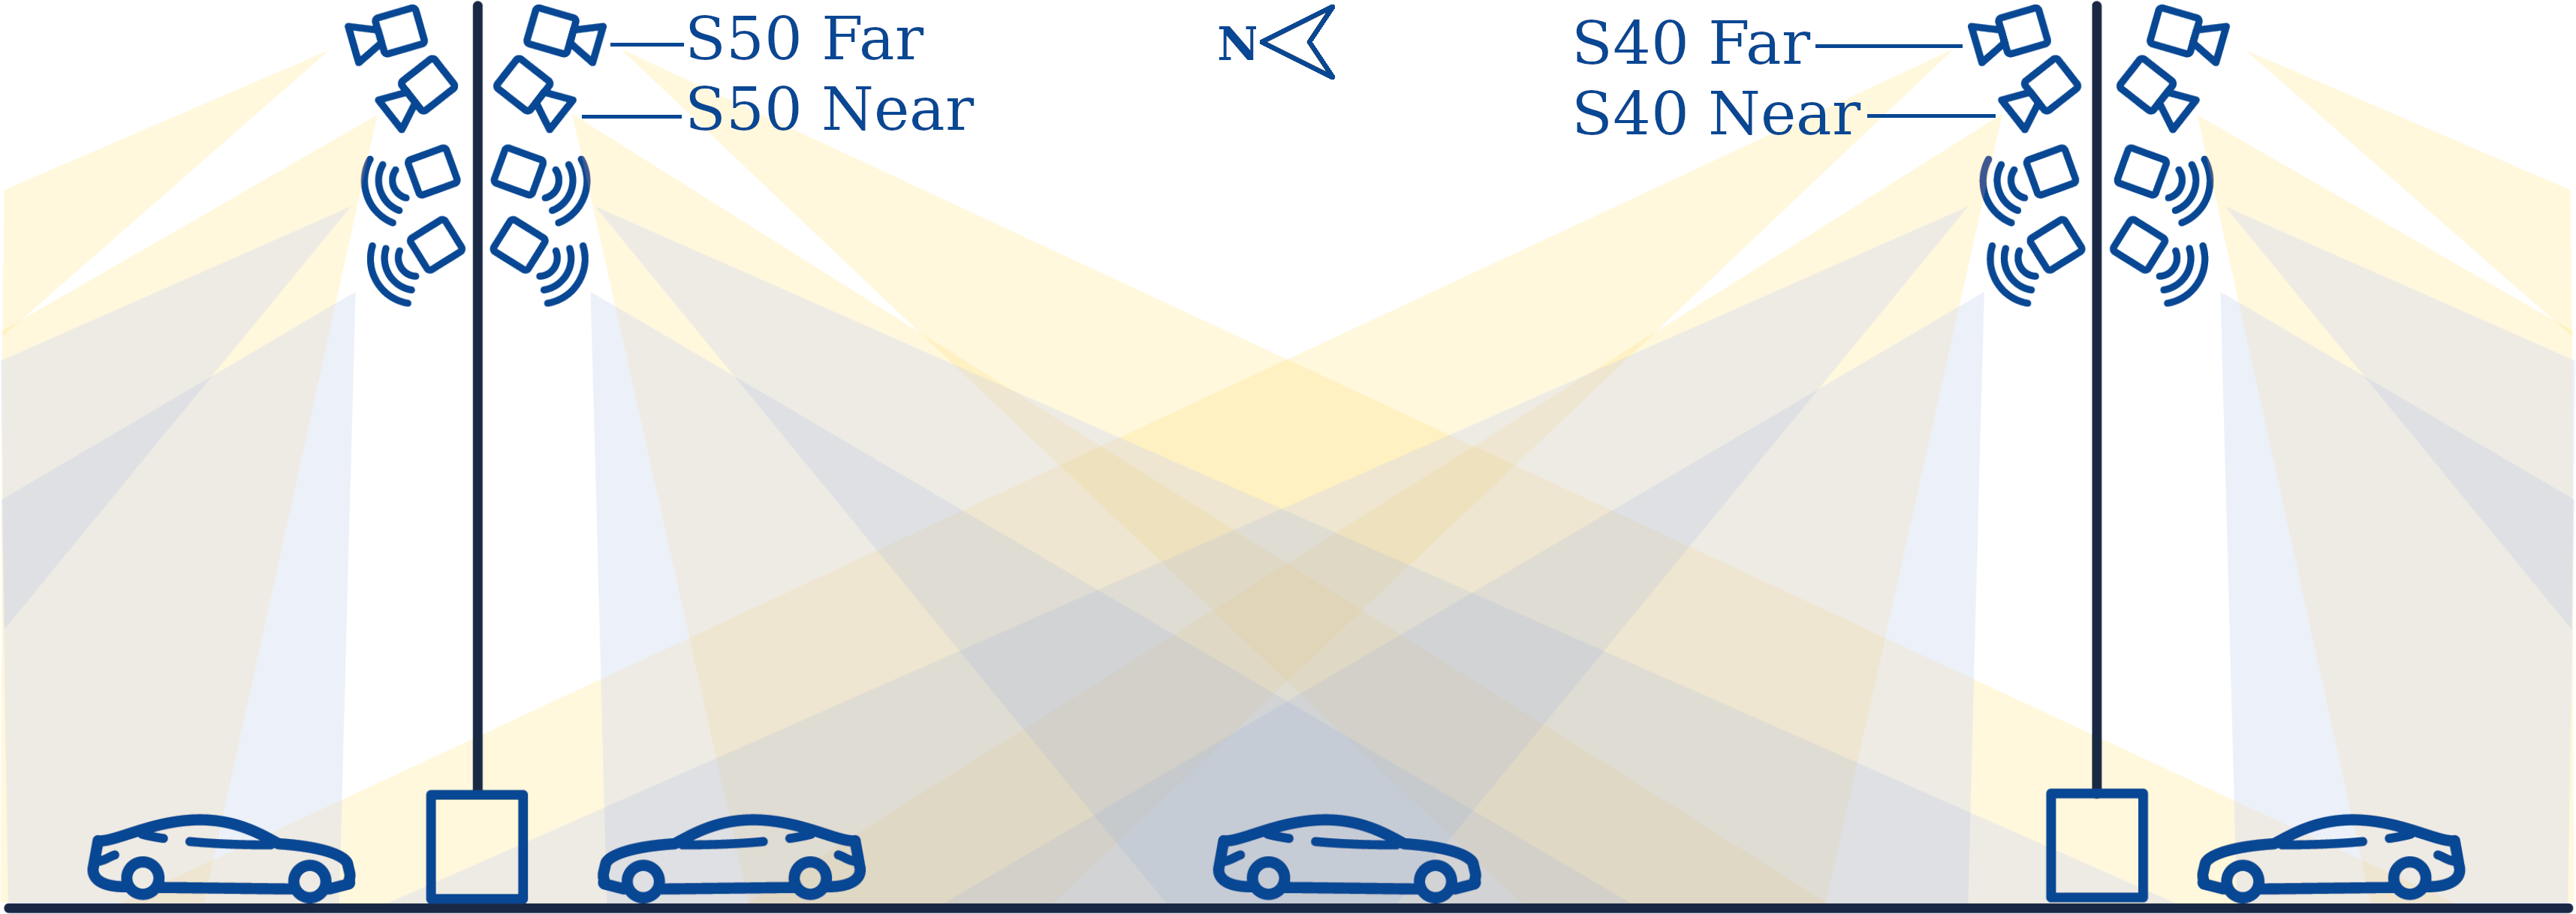
\includegraphics[width=\linewidth]{images/cameras_schema.png}
    \end{center}
       \caption{The schematic camera setup along the highway A9.
       The cameras \camsf{4} and \camsn{4} are facing north,
       the cameras \camsf{5} and \camsn{5} are facing south.}
    \label{fig:cameras_schema}
    \end{figure}

We use video recordings from the four cameras mounted to the two gantry bridges internally named S40 and S50. The schematic camera setup is displayed in \autoref{fig:cameras_schema}.

The dataset consists of four recordings, each with of a length of $1495$ frames over $\sim 60$ seconds at $25$ frames per second.

The recordings are taken on a day with strong winds to ensure high jitter in the video feed to optimally test the Dynamic Stabilization algorithm described in \autoref{sec:dynamic_stabilization_approach}. 

\subsection{Dynamic stabilization}
\label{sec:evaluation_dynamic_stabilization}
To evaluate the Dynamic Stabilization algorithm described in \autoref{sec:dynamic_stabilization_approach} we have come up with two metrics to quantify the environmental influences.

\subsubsection{Optical Flow}
\begin{figure*}[!ht]
    \centering
    \begin{tabular}{cc}
      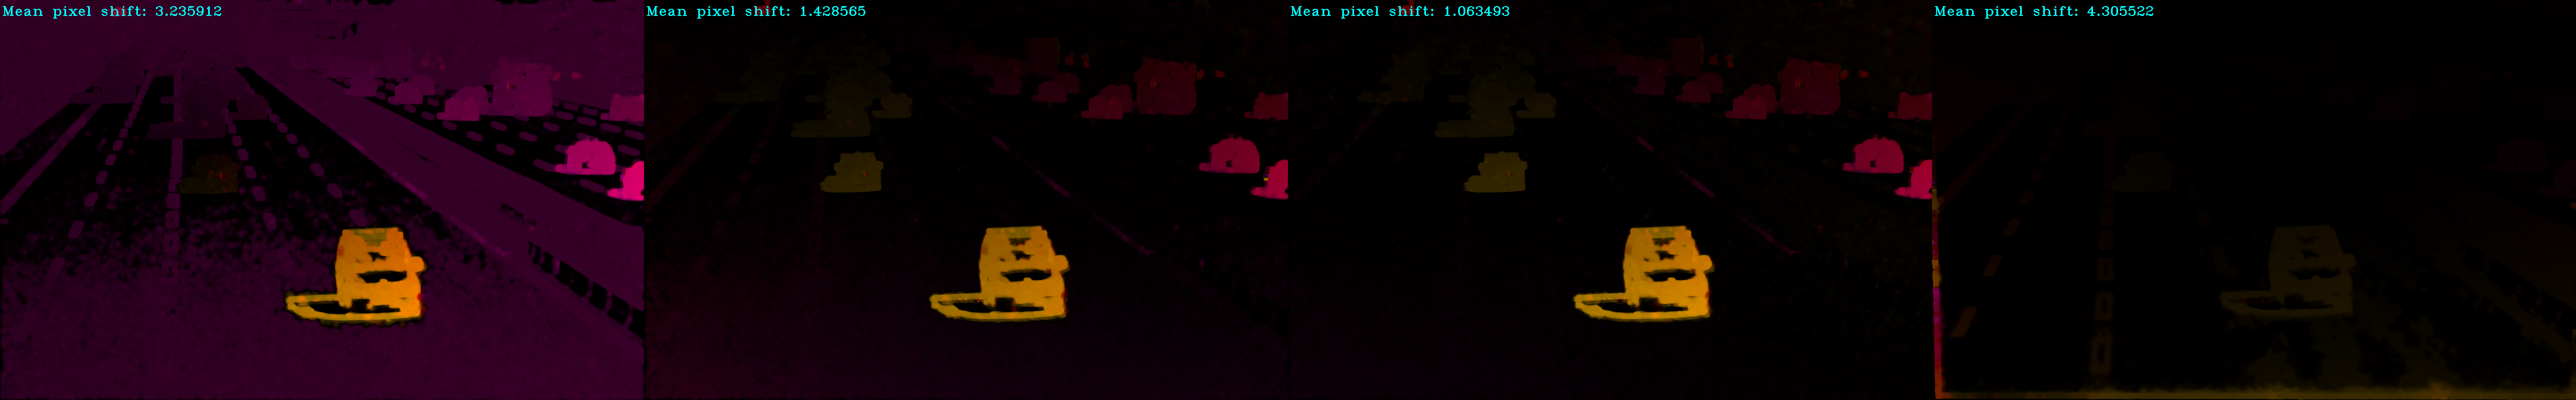
\includegraphics[width=0.95\linewidth]{images/frame_1317_cropped.png}    &  
    \end{tabular}
    \caption{
        The dense Optical Flow displaying the pixel displacement.
        The lighter the color the further the displacement. 
        The angle of displacement is color coded according to the HSV color circle.  
        From left to right: Original frame, 
        stabilized using SURF \cite{bay10.1007/11744023_32,opencv_library} feature detector,
        ORB \cite{rublee6126544, opencv_library} feature detector and
        FAST \cite{Ghahremani_2021,opencv_library} feature detector with FREAK \cite{alahi6247715,opencv_library} feature descriptors.
        In the original frame the violet background color indicates a jittery camera movement. 
        The car in the lower half is driving in the opposite direction as the camera jitters. 
    }
    \label{fig:optical_flow_example}
\end{figure*}

The Optical Flow describes the apparent motion of image objects between two consecutive frames. 
It is a 2D vector field where each vector is a displacement vector showing the movement of points between the frames caused by movement of the objects or cameras.

We use the dense Optical Flow estimation algorithm proposed by Farnebäck \cite{farnback10.1007/3-540-45103-X_50,opencv_library} to measure the displacement of each pixel between the frames. 
We calculate the mean displacement over the whole image to get the overall displacement. 
\autoref{fig:optical_flow_example} shows one frame of Optical Flow calculated.

We see that the dynamically stabilized video feed exhibit a substantially lower mean displacement between frames as the displacement from camera jitter is removed.
This leaves us with only the expected displacement resulting from moving objects, \eg{} vehicles on the highway or shaking trees.

\begin{figure*}[!ht]
    \centering
    \begin{tabular}{cc}
      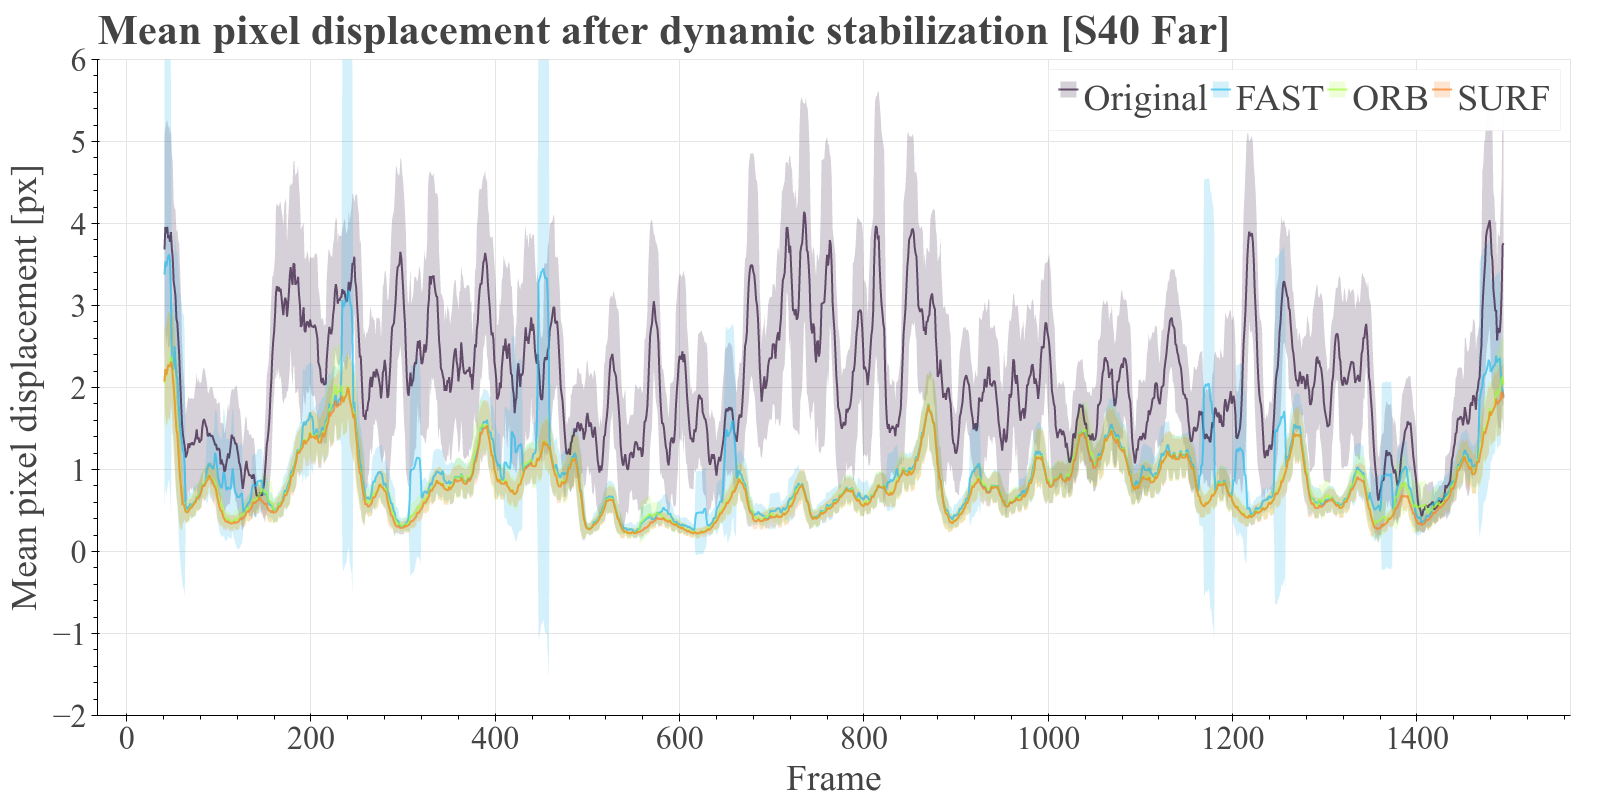
\includegraphics[width=0.475\linewidth]{diagrams/optical_flow/mean_pixel_shifts_after_dynamic_stabilization_s40_far.png}    &  
      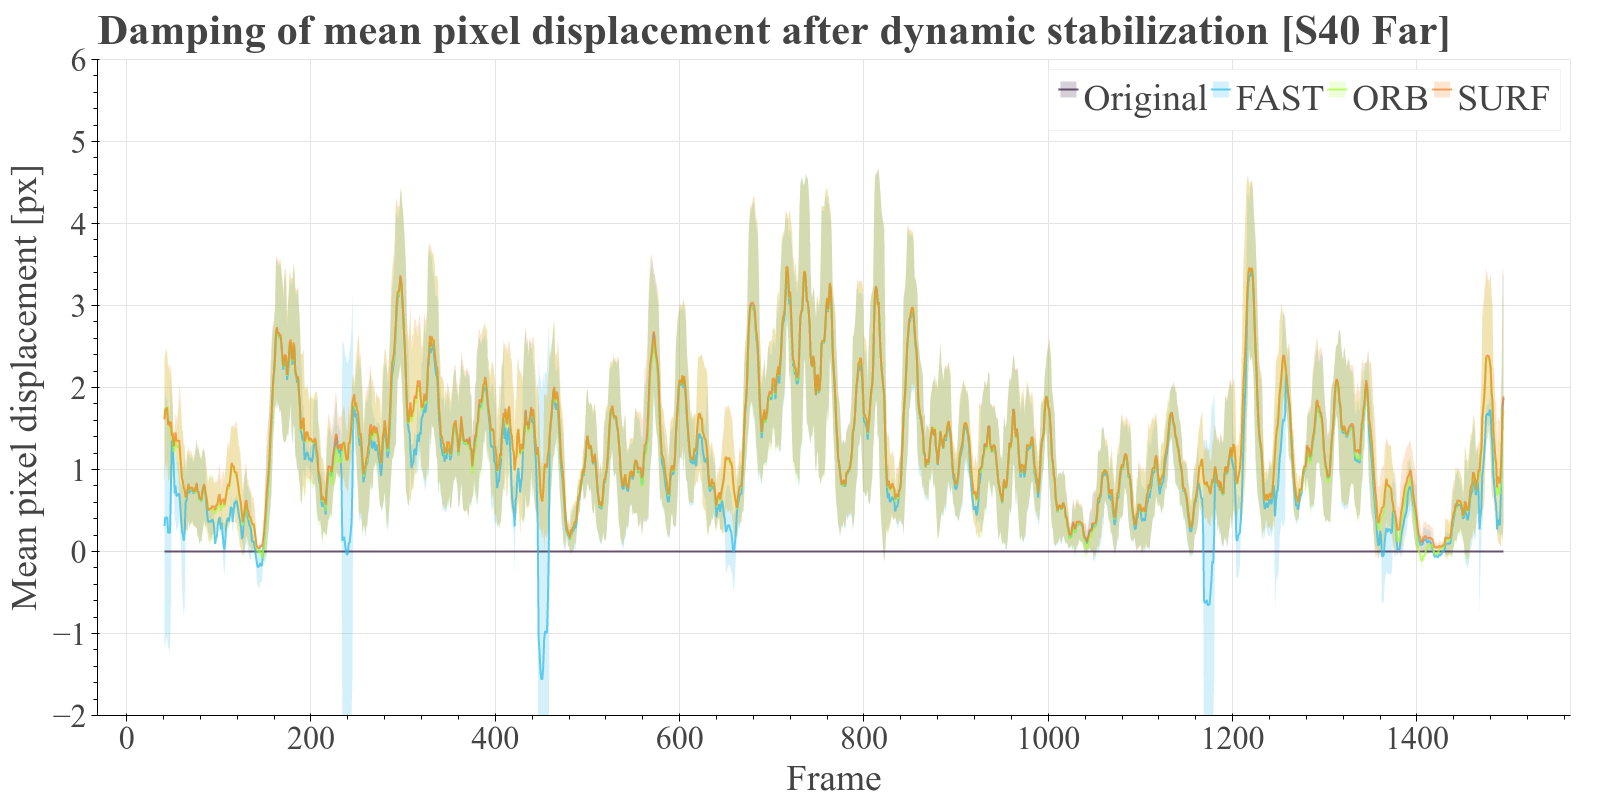
\includegraphics[width=0.475\linewidth]{diagrams/optical_flow/damping_mean_pixel_shifts_after_dynamic_stabilization_s40_far.png}    
\end{tabular}
    \caption{Left: 
        Comparison of the three implemented dynamic stabilizers and the original not stabilized video feed using Optical Flow as metric (lower is better).
        The stabilizers are based on the 
        FAST \cite{Ghahremani_2021,opencv_library} feature detector with FREAK \cite{alahi6247715,opencv_library} feature descriptors,
        SURF \cite{bay10.1007/11744023_32,opencv_library} feature detector and
        ORB \cite{rublee6126544, opencv_library} feature detector.
        The graphs display the mean pixel shift at each frame. 
        Right: 
        The damping capabilities of the same three stabilizers (higher is better). 
        The graphs approximate the removed jitter in the mean pixel shift between the original video and the stabilizer at each frame.\\
        For visualization the values are filtered using the rolling mean over 12 frames. 
        The light areas display the standard deviation within the window.
    }
    \label{fig:dynamic_stabilization_s40_far}
\end{figure*}

\autoref{fig:dynamic_stabilization_s40_far} displays the mean pixel displacement per frame.
It shows that the displacement with especially the SURF \cite{bay10.1007/11744023_32,opencv_library} feature detector is lowered greatly. 
The damping approximates the removed jitter and also displays a huge lowering in mean displacement.


\begin{figure}[!ht]
      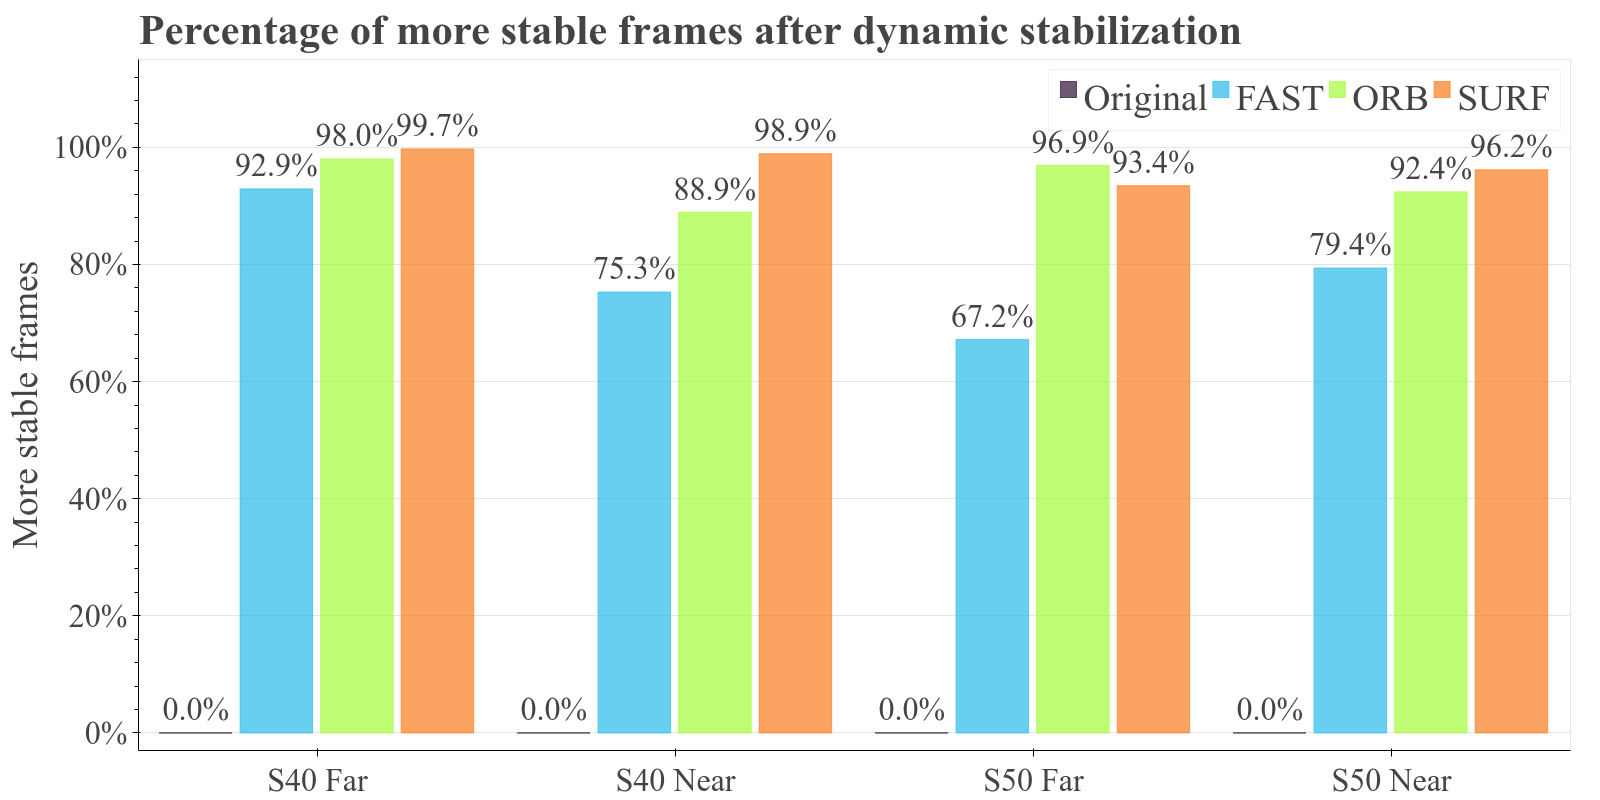
\includegraphics[width=\linewidth]{diagrams/optical_flow/stats.png}    
    \caption{
        Comparison of the percentages of more stable frames after dynamic stabilization per camera and stabilizer.
        A frame is classified as more stable if the mean pixel displacement is lower as in the original video feed. 
        The comparison shows that the stabilizers all improve the video stability, but the SURF \cite{bay10.1007/11744023_32,opencv_library} feature detector based stabilizer outperforms the others.          
    }
    \label{fig:dynamic_stabilization}
\end{figure}

\autoref{fig:dynamic_stabilization} further quantifies the stabilization of the frames.

\paragraph{Problem of Optical Flow as a metric}
\label{sec:evaluation_dynamic_stabilization_optical_flow_problem}
Unfortunately, Optical Flow exhibits one major problem as a metric: 
It cannot distinguish between dynamically moving objects and static scene.
This especially introduces a problem when a jitter of the camera moves the pixels in the same direction as the vehicles path is pointing in image space.
By this jitter the movement of the camera blurs the movement of the dynamic objects into the background and thus removes some of the real movement.
This shows some frames after stabilization to be worse than before. 
This should be taken with caution as the Optical Flow cannot detect the relative motion and thus is not a definite measure for the jitter.
Nonetheless it gives a good hint at the overall stabilization capabilities and can become a measure together with the following measure of the path length of a pixel on a dynamic object. 

\subsubsection{Track features and calculate path smoothness}
To overcome the problems of the Optical Flow as a measure of stability we randomly took three sample vehicles per camera and tracked their pixel locations over time.
As the vehicles move the bounding box of the object is found using the Discriminative Correlation Filter With Channel and Spatial Reliability proposed by Lukezic \etal{} \cite{Lukezic_2017_CVPR,opencv_library}.
The middle point of the bounding box is then written to disk and used as the predicted pixel location of the object.

We only track in the original frame to remove inaccuracies in the tracking and use the homographic transformation matrix from \autoref{eq:homographic_transformation} that stabilizes the frame.
This gives us comparable results for the pixel locations. 

To calculate the arc length we use the sum of distances between the middle point pixel locations over frames. 
The middle point is formulated as 
\begin{equation}
    p = \begin{pmatrix}
        x + 0.5 * w \\
        y + 0.5 * h
    \end{pmatrix}
\end{equation}
with $x$ being the $x$-coordinate of the top left corner of the bounding box, 
$y$ being the $y$-coordinate of the top left corner of the bounding box, 
$w$ being the width of the bounding box and
$h$ being the height of the bounding box.

The arc length is described by
\begin{equation}
    arc(vehicle) = \sum_{n = 1}^{\left\lvert frames \right\rvert } \left\lVert 
        p_{i} - p_{i-1}
    \right\rVert _2
\end{equation} 

To get comparable results a normalization is performed by the arc length of the original video frame.
\begin{equation}
    narc_{stabilizer}(vehicle) = 
    \frac{arc_{stabilizer}(vehicle)}{arc_{original}(vehicle)}
\end{equation} 

\autoref{fig:object_tracking_s40_n_far} displays the vehicles tracked in the video sequence taken from the camera \camsn{4}. 
There is one red truck, a black pickup and a white car taken as a random sample.
The tracking is performed als long as they are visible.

As our dynamic stabilization algorithms remove environmental influences from the frames the pixels only move on the projected path of their vehicles.
\autoref{fig:object_tracking_s40_n_far} displays that the arc lengths after stabilization remain at only a relative length of $0.5$ of the original length.
This clearly indicates that with the same vehicle movement the tracked position is much more accurate.

\begin{figure*}[!ht]
    \centering
    \begin{tabular}{cc}
      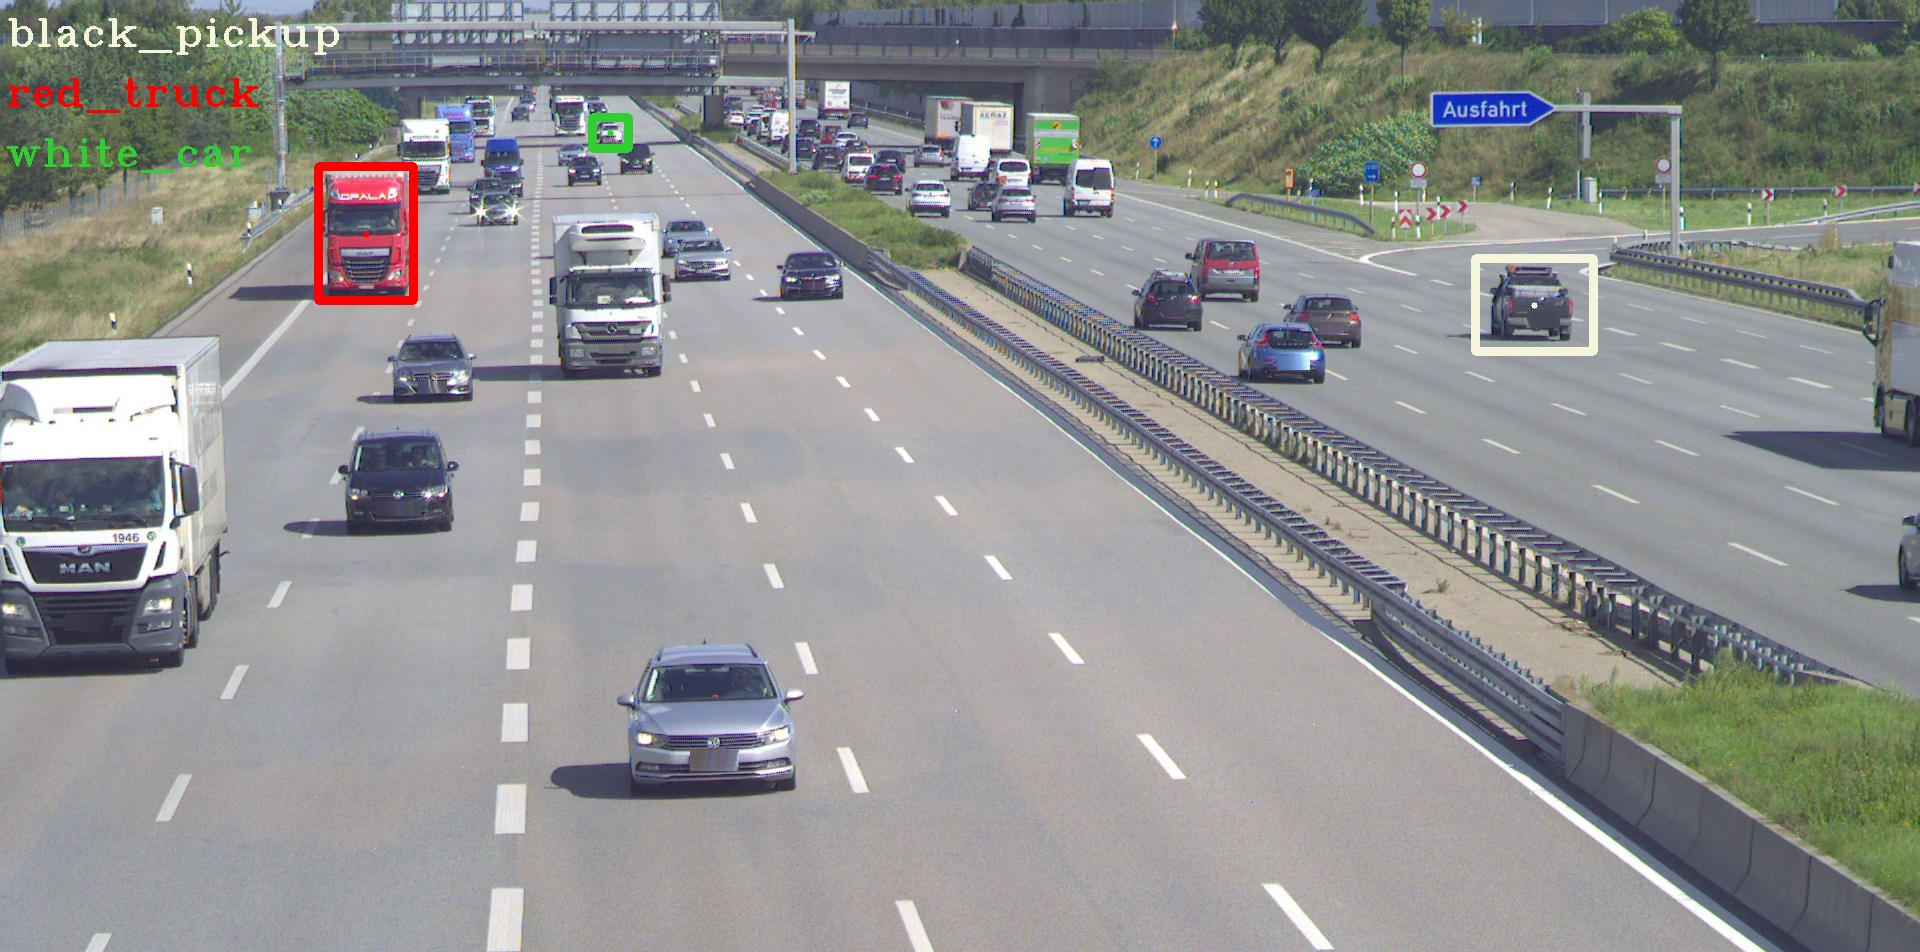
\includegraphics[width=0.475\linewidth]{diagrams/object_tracking/s40_n_far/frame_cropped.png}    &  
      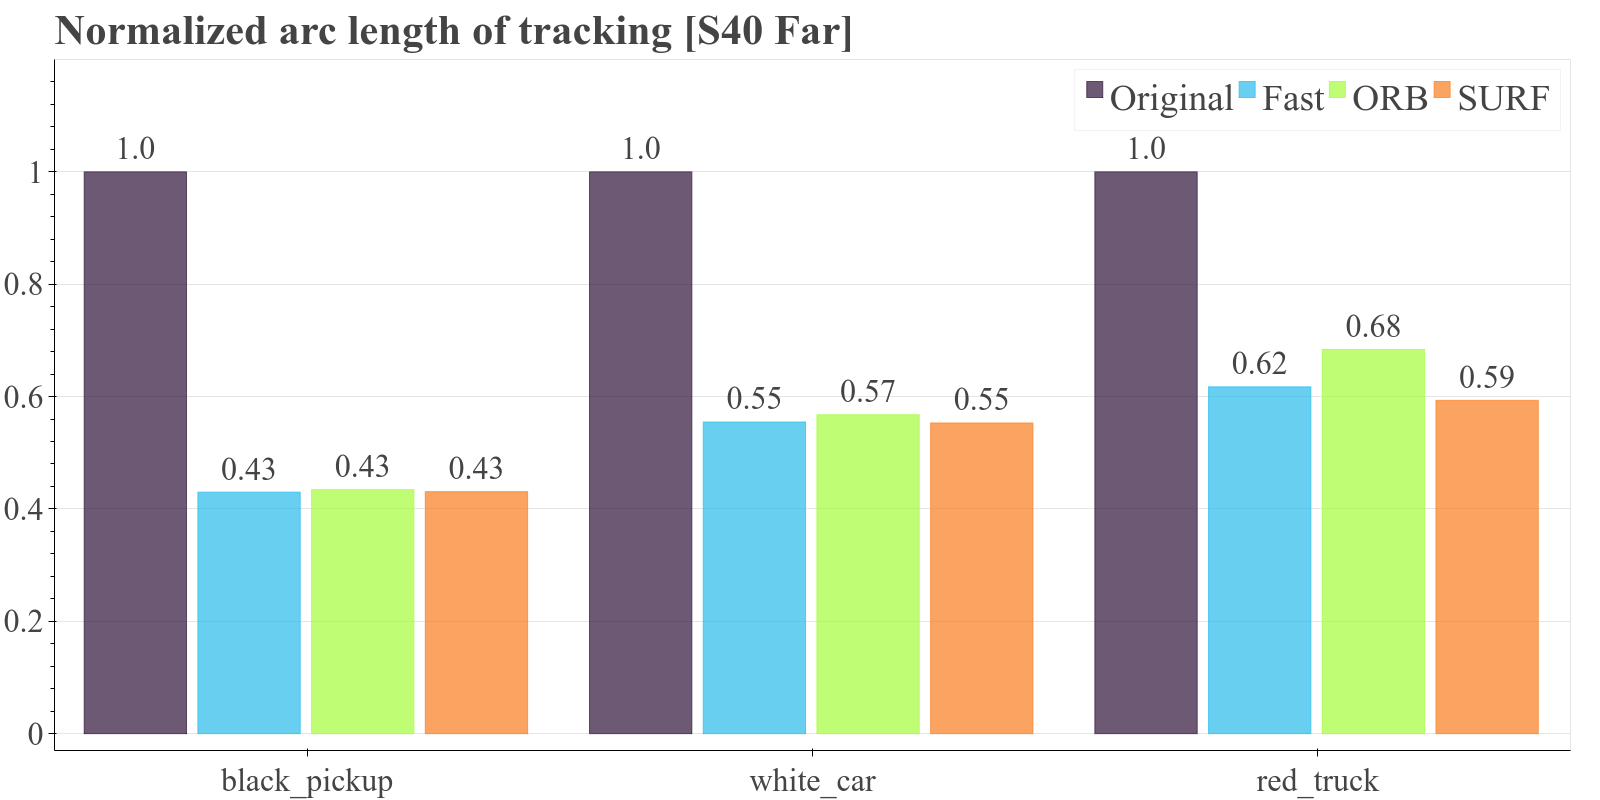
\includegraphics[width=0.475\linewidth]{diagrams/object_tracking/s40_n_far/arcs.png}    
\end{tabular}
    \caption{Left: 
    The exemplary vehicles tracked through the video sequence of the camera \camsn{4}. 
    Right:
    The corresponding normalized arc lengths of the pixel path. 
    The length is normalized by the original arc length, hence the 1.0 factor for the original video. 
    As the jitter is removed, the pixels movement is lowered significantly as it does only move with the vehicle, not the camera.
    This can be seen with around half of the path length remaining after stabilization for all stabilizers.
    }
    \label{fig:object_tracking_s40_n_far}
\end{figure*}

The 
\autoref{fig:object_tracking_appendix_s40_n_far}, 
\autoref{fig:object_tracking_appendix_s40_n_near}, 
\autoref{fig:object_tracking_appendix_s50_s_far} and 
\autoref{fig:object_tracking_appendix_s50_s_near} in \autoref{sec:appendix} display the tracked pixel locations of three cars per camera.

\subsubsection{Speed comparison}
% !TEX root=./report.tex

\subsection{Static calibration}
In the following we evaluate the implemented static calibration algorithm and assess the algorithmic and systematic errors.

\subsubsection{Ensure no Systematic Error}

\begin{figure*}[t]
    \centering
    \begin{tabular}{cc}
      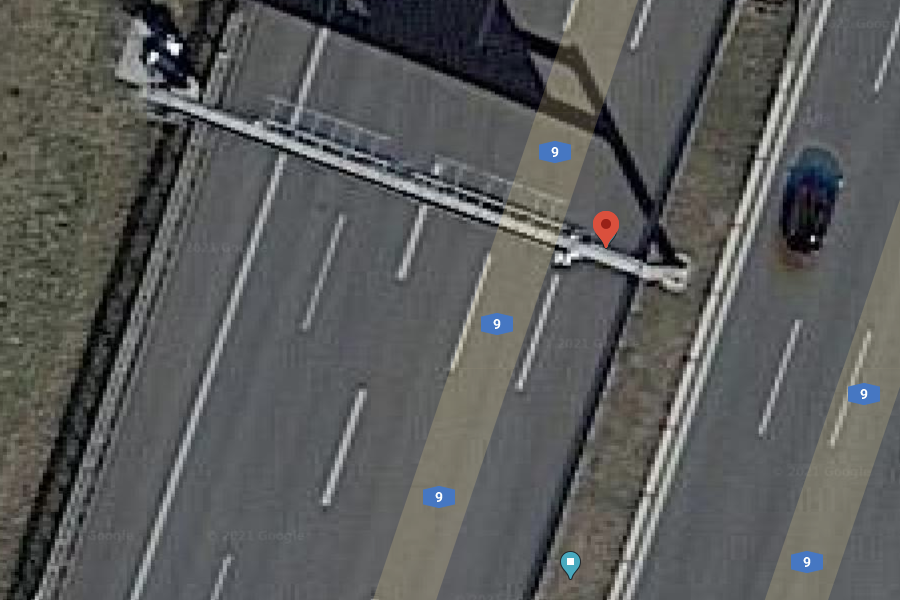
\includegraphics[width=0.45 \linewidth]{images/calibration/google_maps_s50_s.png} &
      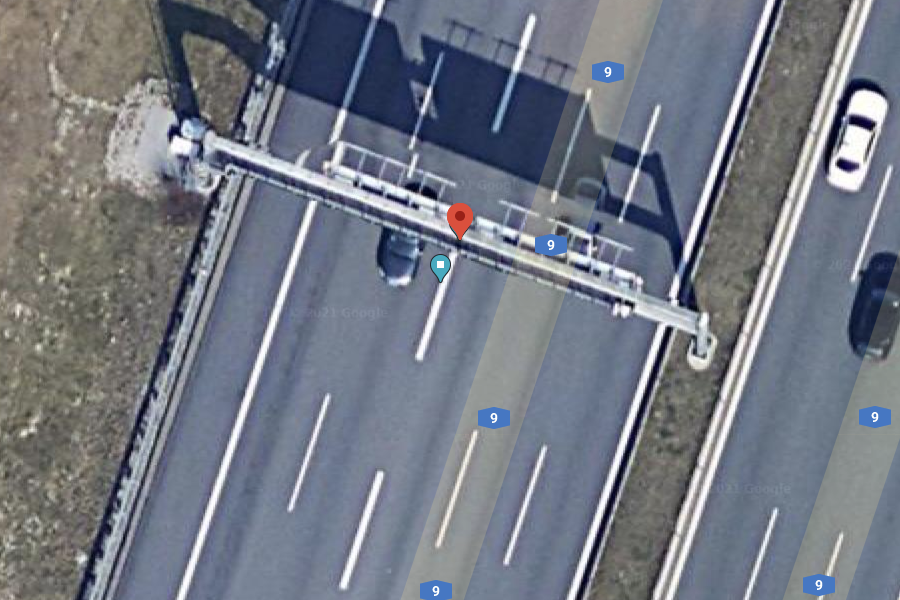
\includegraphics[width=0.45 \linewidth]{images/calibration/google_maps_s40_n.png} 
  \end{tabular}
  \caption{Left: The positions of the cameras \camsn{4} (red) and \camsf{4} (green) and their respective looking directions (yellow). 
  Right: The positions of the cameras \camsn{5} (red) and \camsf{5} (green) and their respective looking directions (yellow). 
  It displays that the rotation of the cameras is in a reasonable range so that the cameras look along the highway as expected. 
  Also the cameras are within reasonable translational bounds around their real world location as \autoref{sec:static_calibration_expectable_error} shows.
  }
  \label{fig:google_maps}
  \end{figure*}

The proposed pose estimation algorithm from \autoref{eq:static_calibration_error} converges to a pair of optimal translation $T$ and rotation $R$ values for the camera pose.
These $T, R$ values approximate the projection from the world objects to the pixels as described in \autoref{eq:static_calibration_reprojection}.

Using a maps provider we assured that the resulting values are within reasonable ranges and that there are no systematic errors in the optimization.
The results are displayed in \autoref{fig:google_maps}

\subsubsection{Points needed for convergence}
The correspondences build up a system of linear equations. 
This system of equations is solvable if there exist a more or equal number of constraints on the parameters than there are degrees of freedoms in the system:
\begin{equation}
  \label{eq:static_calibration_reprojection_evaluation}
  p_c = \pi \left(  
    % \begin{bmatrix}
    %   R, T \\
    %   0, 1
    % \end{bmatrix} *
    R * T *
    (o_c + \lambda_c * h_c)
  \right), \forall c \in C
\end{equation}
This is the case if:
\begin{equation}
  \begin{split}
  2 * \left\lvert C \right\rvert \quad \geq& \quad 5 + 3 + 3 + 1 * \left\lvert C \right\rvert \\
  \left\lvert C \right\rvert \quad \geq& \quad 11 
\end{split}
\end{equation} 

As each of the pixel per correspondence gives us two constraints and we optimize over the 5 intrinsic parameters (\autoref{eq:static_calibration_intrinsic_parameters}), the 3 extrinsic translation, 3 extrinsic rotation parameters and one $\lambda$ parameter per correspondence.
We see that 11 points are enough to recover the pose.

\subsubsection{Structure of points}
The best result are shown when there are at least two correspondences per object.
These correspondences should be the top and bottom most visible pixel of the object.
If there exists only 1 or a low number of near pixels, the algorithm cannot precisely recover the camera pose, as it is free to move the correspondence along the center line of the object.
The algorithm therefore cannot distinguish the solutions where the camera is placed low, thus projecting a high point of an object to a low pixel correspondence, 
or if it should place the camera higher and lower the correspondences world position along the center line.

We thus conclude that the best solution is recovered the more the pixels fill the whole object, and the more spread to the top and bottom of the object the correspondences are. 




























\subsubsection{Expectable Error Bounds}
\label{sec:static_calibration_expectable_error}

Due to measurement uncertainty in the camera sensors we expect some remaining error after pose estimation.
To conclude a lower bound on this error we start from the optimized focal length $f_px$ in pixels and the sensor width $w_{mm}$ in millimeters and $w_{px}$ in pixels.

The focal length in millimeters is given by 
\begin{equation}
  f_{mm} = f_{px} * \frac{w_{mm}}{w_{px}}
\end{equation}

We then calculate the field of view (FOV) in radians by 
\begin{equation}
  FOV_x = 2 * \arctan \left(\frac{f_{mm}}{2 * w_{mm}}\right)
\end{equation} 
Equivalent the $FOV_y$ with the height of the sensor $h_{mm}$.

This brings us to a formulation for the angle spanned by each pixel
\begin{equation}
  \alpha_{px} = \frac{w_{px}}{FOV_x}
\end{equation} 

Using the pythagorean formula we can then calculate the uncertainty $u$ in meters of the camera as the spanned meters per pixel relative to the distance $d$ from the camera 
\begin{equation}
  u = \tan (\alpha_{px}) * d
\end{equation}

\begin{table}
  \begin{center}
    \begin{tabular}{ |c | c | c| c| c| c |}
      \hline
      Camera & $f_{px}$ & $FOV_x [^{\circ}]$ & $\alpha_{px}$ & $d [m]$ & $u [cm]$ \\
      \hline
      \camsf{4} & 8591 & 12.753 & $1.16e^{-4}$ & 200 & 2.32 \\
      \camsf{4} & 8591 & 12.753 & $1.16e^{-4}$ & 650 & 7.54 \\
      \hline
      \camsn{4} & 2735 & 38.678 & $3.52e^{-4}$ & 25 & 0.88 \\
      \camsn{4} & 2735 & 38.678 & $3.52e^{-4}$ & 450 & 15.82 \\
      \hline
      \camsf{5} & 8868 & 12.357 & $1.12e^{-4}$ & 200 & 2.22 \\
      \camsf{5} & 8868 & 12.357 & $1.12e^{-4}$ & 650 & 7.30 \\
      \hline
      \camsn{5} & 2747 & 38.527 & $3.50e^{-4}$ & 25 & 0.88\\
      \camsn{5} & 2747 & 38.527 & $3.50e^{-4}$ & 450 & 15.76 \\
      \hline
    \end{tabular}
  \end{center}
  \caption{
    \label{tab:static_calibration_camera_uncertainty}
  }
\end{table}

\autoref{tab:static_calibration_camera_uncertainty} displays the uncertainty for our cameras.
It shows that the far cameras cannot distinguish between points that are $\sim 2.2 cm$ at the nearest visible distance from the camera ranging up to $\sim 7.54 cm$ at the farthest distance.
The near cameras cannot distinguish between points that are $\sim 0.88 cm$ at the nearest visible distance from the camera ranging up to $\sim 15.82 cm$ at the farthest distance.

This gives a lower bound for the uncertainty in the translational parameters of the camera.
The camera translation cannot be more precise as the lowest uncertainty in the measurements.
Nonetheless, in practice the error will sum up and the translation parameters will drift inevitable. 

This concludes that objects near to the camera are more reliable to detect and to use for estimation.





















\subsubsection{Expectable Deviations among Estimations}
The proposed pose estimation algorithm is based on the minimization of the reprojection-error \autoref{eq:static_calibration_reprojection}.
As with all optimization problems convergence is reached when the values that are optimized don't change anymore.

The optimization jointly optimizes for the 6 camera parameters, 3 for the translation, 3 for the Euler angle rotation and one $\lambda$ parameter per correspondence.
The resulting high-dimensional problem exceeds multiple minima, whereas each represents a configuration for the camera pose that well explains the dependency between pixels, world objects and the camera. 

As stated previously the loss landscape does exhibit a multitude of local minima, thus the optimization procedure converges to different sets of parameters. 

\begin{figure}[t]
  \centering
  \begin{tabular}{cc}
    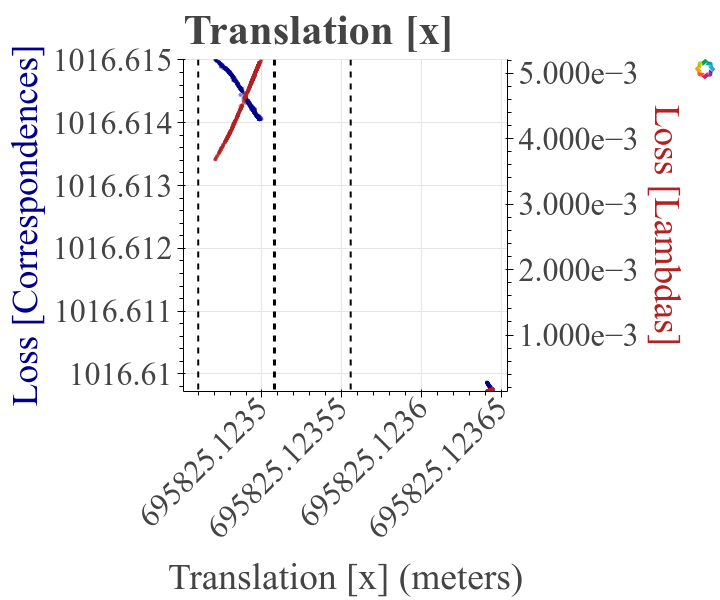
\includegraphics[width=0.45 \linewidth]{diagrams/calibration/s40_n_far_small/parameters_all.csv/Translation[x]_vs_Loss[Correspondences]_vs_Loss[Lambdas]_cluster_All.png} &
    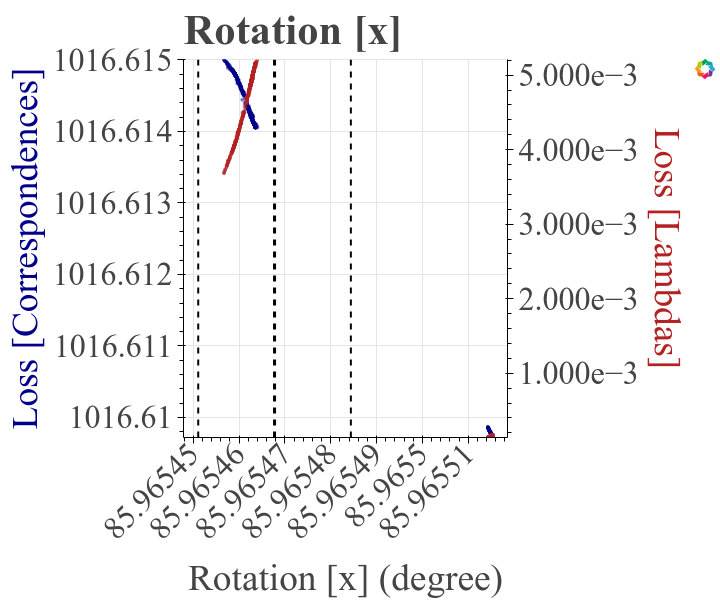
\includegraphics[width=0.45 \linewidth]{diagrams/calibration/s40_n_far_small/parameters_all.csv/Rotation[x]_vs_Loss[Correspondences]_vs_Loss[Lambdas]_cluster_All.png} \\
    
    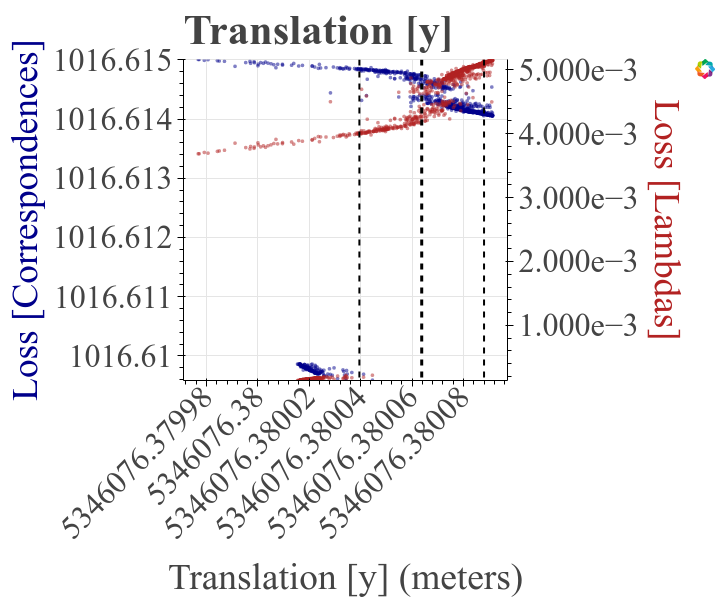
\includegraphics[width=0.45 \linewidth]{diagrams/calibration/s40_n_far_small/parameters_all.csv/Translation[y]_vs_Loss[Correspondences]_vs_Loss[Lambdas]_cluster_All.png} &
    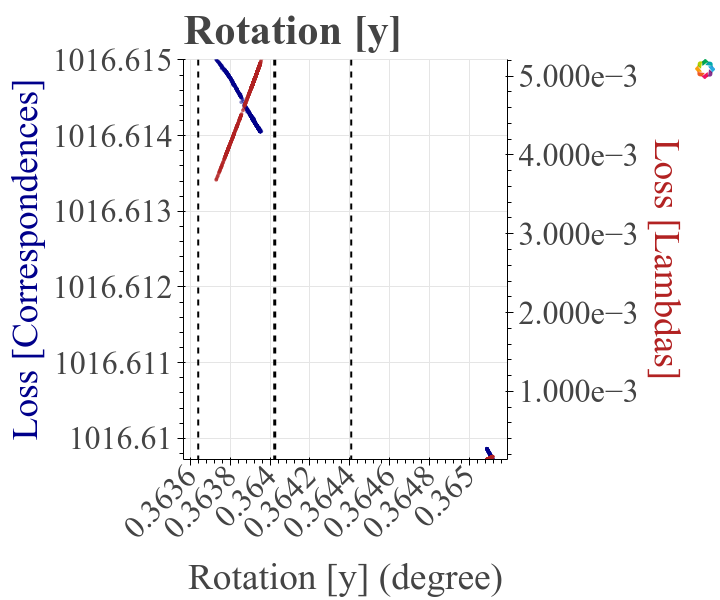
\includegraphics[width=0.45 \linewidth]{diagrams/calibration/s40_n_far_small/parameters_all.csv/Rotation[y]_vs_Loss[Correspondences]_vs_Loss[Lambdas]_cluster_All.png} \\
    
    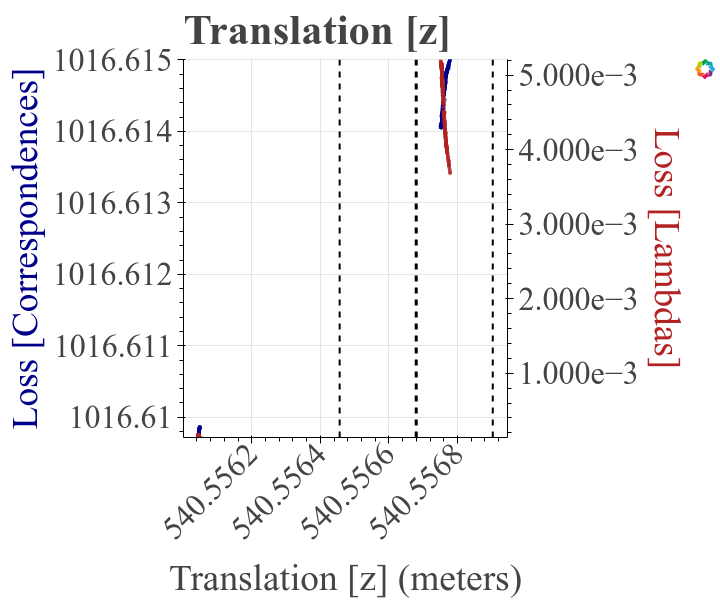
\includegraphics[width=0.45 \linewidth]{diagrams/calibration/s40_n_far_small/parameters_all.csv/Translation[z]_vs_Loss[Correspondences]_vs_Loss[Lambdas]_cluster_All.png} &
    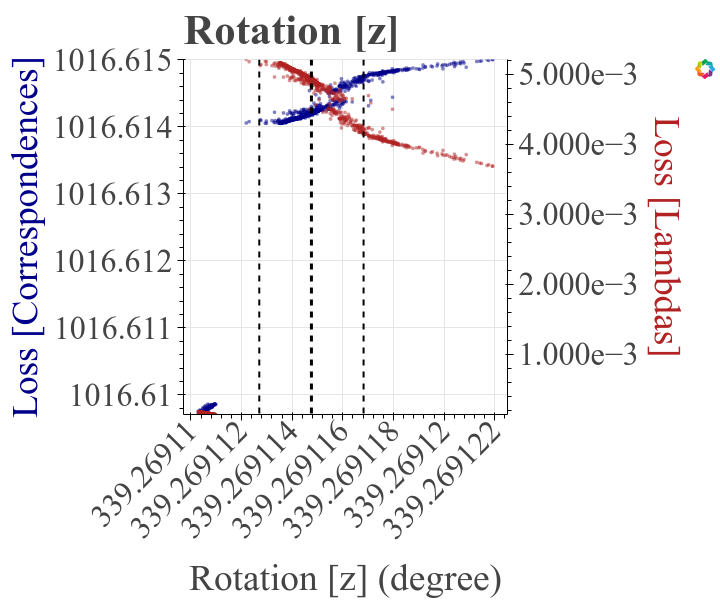
\includegraphics[width=0.45 \linewidth]{diagrams/calibration/s40_n_far_small/parameters_all.csv/Rotation[z]_vs_Loss[Correspondences]_vs_Loss[Lambdas]_cluster_All.png} \\
\end{tabular}
\caption{
  Left: The resulting translational parameters plotted against the remaining losses. 
  Right: The resulting rotational parameters plotted against the remaining losses.
  The mean of the distributions is displayed as thick dashed line. The smaller dashed lines display the standard deviation $\sigma$.
  The $\sigma$ of the translations does not exceed $2 * 10^{-4} m = 0.2 mm$.
  For the rotation $\sigma$ is at most $4 * 10^{-4} deg$.
  }
\label{fig:static_calibration_algorithmic_error}
\end{figure}

\autoref{fig:static_calibration_algorithmic_error} displays the resulting parameters for the camera \camsf{4}.
We plot the loss of the correspondence residuals and the $\lambda$ residual blocks against each of the parameters.
The translation parameters are in meters and relative to the transverse mercator projection \cite{lambert1894anmerkungen}.
The rotation parameters are in degree of Euler angles.

The plots show that the standard deviation $\sigma$ of the translations does not exceed $2 * 10^{-4} m = 0.2 mm$.
For the rotation $\sigma$ is at most $4 * 10^{-4} deg$. 

We have shown the expectable error for the parameters resulting from the sensor and map inaccuracies in \autoref{sec:static_calibration_expectable_error}. 
We conclude that in relation to these the algorithmic error can be neglected.

In the appendix \autoref{sec:appendix} we additionally evaluate the other cameras.

% \subsubsection{Minimal number of correspondences}

% !TEX root=./report.tex

\section{Future Work}
The project leaves us with the opportunity to continue the research in multiple directions.

\subsection{Varying Weather and Lighting Conditions}
We tested and evaluated the implementations on recordings with good weather and lighting conditions, thus a next step is to test the implementations in bad weather and lighting conditions, \eg by night, rain and snow.
From out current perspective the feature based dynamic stabilization approach will suffer in performance as the homography estimation depend on features in the image space. 
By night and if the static background is occluded the stabilization pipeline will fail, although in these cases the complete RGB image will be unusable at all.

We implemented the solver for the BA problem to include human interaction when mapping from PDs to pixels.
The mapping will be harder in bad weather and lighting conditions based on the worse visibility of the landmarks.
We propose an automatic mapping scheme in \Cref{sec:auto_mapping_landmarks}.
This scheme will be affected by changing weather and lighting conditions as the detection of new landmarks is also based on the visibility of landmarks.

%%%%%%%%%%%%%%%%%%%%%%%%%%%%%%%%%%%%%%%%%%%%%%%%%%%%%%%%%%%%%%%%%%%%%%%%%%%%%%%%%%%%%%%%%%%%%%%%%%%%%%%%%%%%%%%%%%%%
%%%%%%%%%%%%%%%%%%%%%%%%%%%%%%%%%%%%%%%%%%%%%%%%%%%%%%%%%%%%%%%%%%%%%%%%%%%%%%%%%%%%%%%%%%%%%%%%%%%%%%%%%%%%%%%%%%%%
%%%%%%%%%%%%%%%%%%%%%%%%%%%%%%%%%%%%%%%%%%%%%%%%%%%%%%%%%%%%%%%%%%%%%%%%%%%%%%%%%%%%%%%%%%%%%%%%%%%%%%%%%%%%%%%%%%%%

\subsection{Dynamic Stabilization}
We present two major improvements that can be done to extend the presented dynamic stabilization approach.

\subsubsection{Warp Field Stabilization Based on Optical Flow}
We use the optical flow to measure the performance of the stabilizers as described in  \Cref{sec:evaluation_dynamic_stabilization_optical_flow}.
The optical flow is a 2D vector field where each vector is a displacement vector showing the movement of pixels between frames caused by movement of the objects or cameras.
The image can be stabilized using the inverse vector field that also minimizes the reprojection error between frames.

\subsubsection{Deep Learning Based Dynamic Stabilization}
Based on the ongoing success of deep learning approaches in computer vision, especially of convolutional neural networks (CNN), a self-learning stabilization procedure might be developed.
The CNN expects the current input and reference frame and outputs the homographic transformation or the warped frame. 
This might speed up the pipeline and inherently adds a measure for the uncertainty of the results by modelling the probability of the homographic transformation.
This approach can be used to fuse the feature detection, matching and warping steps into one joint step that is learned by the CNN from labeled data.

%%%%%%%%%%%%%%%%%%%%%%%%%%%%%%%%%%%%%%%%%%%%%%%%%%%%%%%%%%%%%%%%%%%%%%%%%%%%%%%%%%%%%%%%%%%%%%%%%%%%%%%%%%%%%%%%%%%%
%%%%%%%%%%%%%%%%%%%%%%%%%%%%%%%%%%%%%%%%%%%%%%%%%%%%%%%%%%%%%%%%%%%%%%%%%%%%%%%%%%%%%%%%%%%%%%%%%%%%%%%%%%%%%%%%%%%%
%%%%%%%%%%%%%%%%%%%%%%%%%%%%%%%%%%%%%%%%%%%%%%%%%%%%%%%%%%%%%%%%%%%%%%%%%%%%%%%%%%%%%%%%%%%%%%%%%%%%%%%%%%%%%%%%%%%%

\subsection{Static Calibration}
We present two major improvements that can be done to extend the presented static calibration approach.

\subsubsection{Robustness Against Outliers}
BA problems are inherently prone to outliers, as they greatly impact the shape of the reprojection-error loss landscape. 
To use the presented system in practice a RANSAC \cite{fischler1981random} or similar sample consensus based approach needs to be implemented.
By evaluating the calibration multiple times with different subsets of correspondences a stable sample consensus can be found in asymptotically all runs.
This will greatly impact the robustness of the calibration procedure against outliers, as they can be filtered out automatically by the algorithm.  


\subsubsection{Fully Automatic Static Calibration}
\label{sec:auto_mapping_landmarks}
We establish the mapping of the correspondences by hand, thus a human has to look up the ids of the landmarks in the HD maps and assign them to their respective pixels.
After an initial calibration that requires human interaction, an image region based approach might be used to automate this mapping.
One can project the known base origin points of the objects from the HD maps into the current frame.
Starting from the projected pixel locations one could search in a defined enclosing region to find pixels that clearly correspond to the objects by applying template, color or gradient matching approaches.
The automatic detection of landmarks enables the system to perform fully automatic static self calibration.

\subsubsection{Machine Learning Based Bundle Adjustment}
Aravkin \etal \cite{students_t_bundle_adjustment} have shown that the BA problem can be modelled on top of a Student's-t distribution. 
The resulting statistical machine learning approach for the BA can be used to jointly estimate the camera parameters and world positions of objects, while at the same time being robust against outliers.
  
\subsubsection{New High Definition Map}
The newer OpenDRIVE standard also provides the possibility to include lane markings.
These lane markings are easily detectable and can be used for the calibration procedure in conjunction with the object landmarks.
This would greatly simplify the automatic detection and mapping procedures as described in \Cref{sec:auto_mapping_landmarks} as they are spatially more extend and thus easier to detect.
Furthermore, the lane markings are always white or yellow which simplifies the detection.
As shown in \Cref{sec:static_calibration_expectable_error} the static calibration is more precise the closer the correspondences are to the cameras. 
As there exists far more lane markings than objects, and with the markings being evenly distributed over the road the static calibration would benefit from this additional information.
% !TEX root=./report.tex

\section{Conclusion}

In this paper we proposed two main improvements on the vision based tracking system used in the \Providentia{}.

We first presented a pipeline to dynamically stabilize jittery motion in the video streams of RGB cameras mounted to gantry bridges along a highway.
We applied a homographic transformation in image space based on the matching of visual features between the current and a stable reference frame.
We have shown that the stabilization substantially (up to $99.8\%$) improves the stability of the frames regarding the remaining mean pixel displacement.
By tracking vehicles through the video sequence we have shown that the remaining length of the pixels path after stabilization is lowered by up to $57\%$ compared to the not stabilized one and thus the jittery motion of the camera is compensated significantly after stabilization.
Finally, we have shown that the dynamic stabilization pipeline is easily realtime capable with at least $50$ processed frames per second.

We secondly presented the formulation of a single camera RGB-only Bundle Adjustment problem that is minimized using the reprojection-error to statically calibrate the camera setup to the reference system.
We recover the cameras pose by jointly optimizing for the cameras intrinsic and extrinsic parameters as well as the real world position of viewed correspondences to a high definition map.
We checked our results for the absence of systematic errors, gave a lower bound on the number of correspondences needed for convergence and the structure the correspondences have to exceed.
We evaluated the expectable error after pose estimation that arises from measurement uncertainties and imprecisions in the HD map and have shown that the deviations among the minima found by the optimization strategy are neglectable.


\newpage
{
    \small
    \bibliographystyle{ieee_fullname}
    \bibliography{bib_literature}
}

% % !TEX root=./report.tex

% \pagebreak
\newpage

\section{Appendix}
\label{sec:appendix}
To declutter the paper we moved some of the images here.

\begin{figure*}[!ht]
  \centering
    \begin{tabular}{cc}
      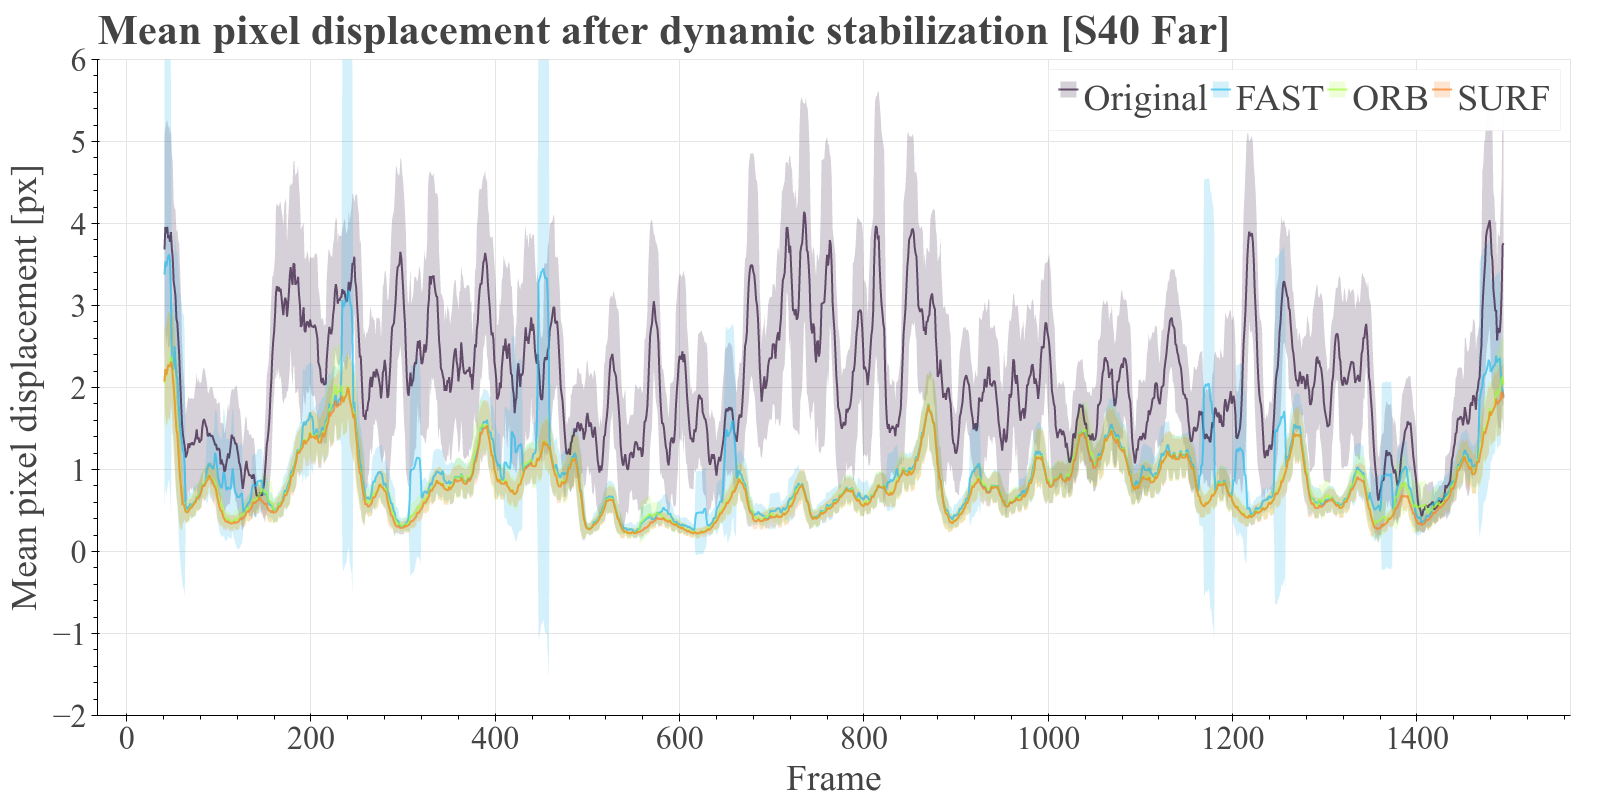
\includegraphics[width=0.475\linewidth]{diagrams/optical_flow/mean_pixel_shifts_after_dynamic_stabilization_s40_far.png}    &  
      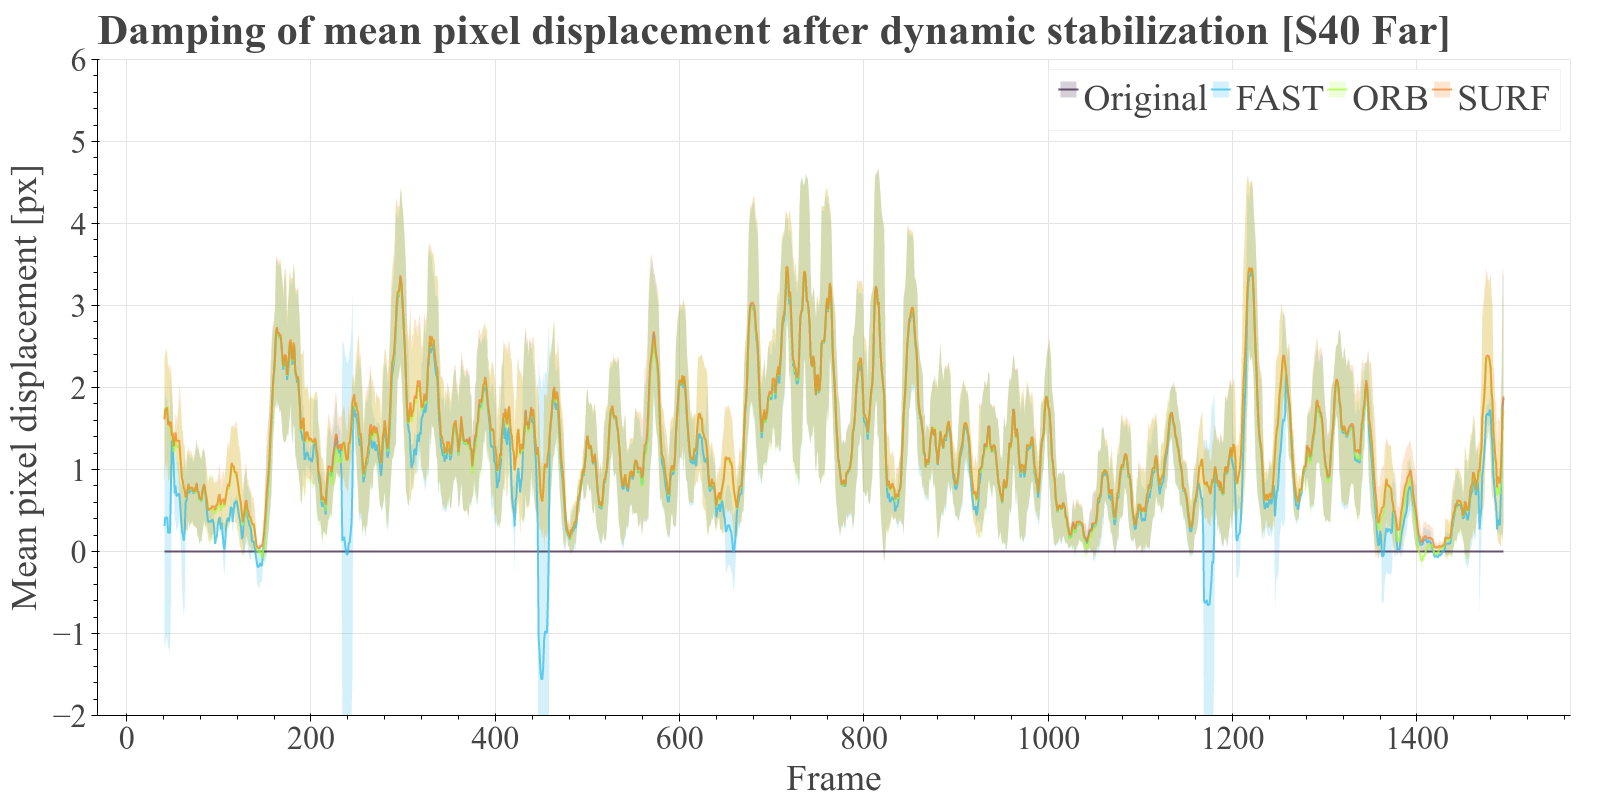
\includegraphics[width=0.475\linewidth]{diagrams/optical_flow/damping_mean_pixel_shifts_after_dynamic_stabilization_s40_far.png}   \\ 

      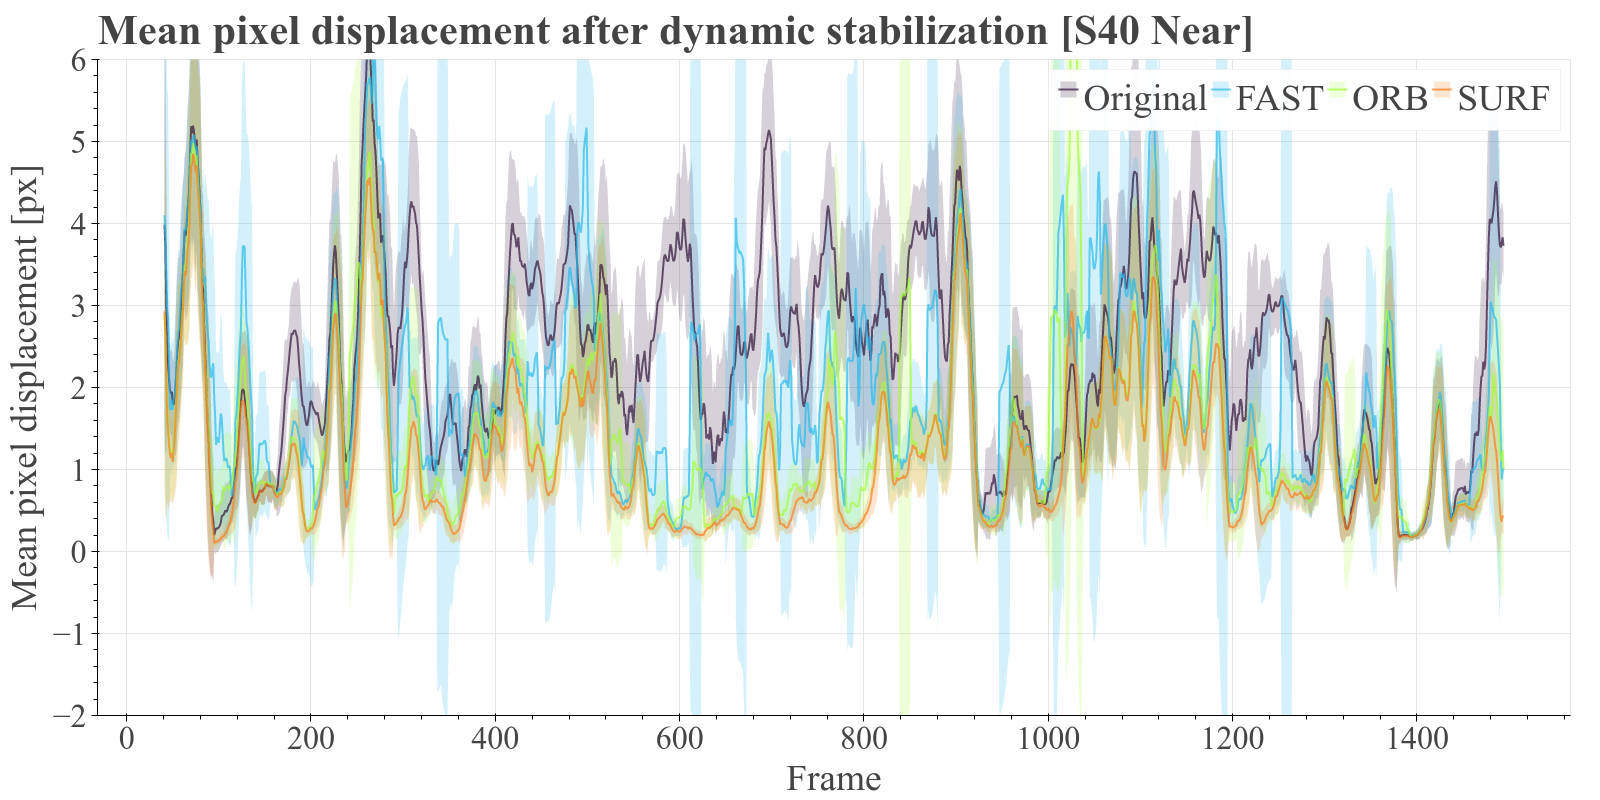
\includegraphics[width=0.475\linewidth]{diagrams/optical_flow/mean_pixel_shifts_after_dynamic_stabilization_s40_near.png}    &  
      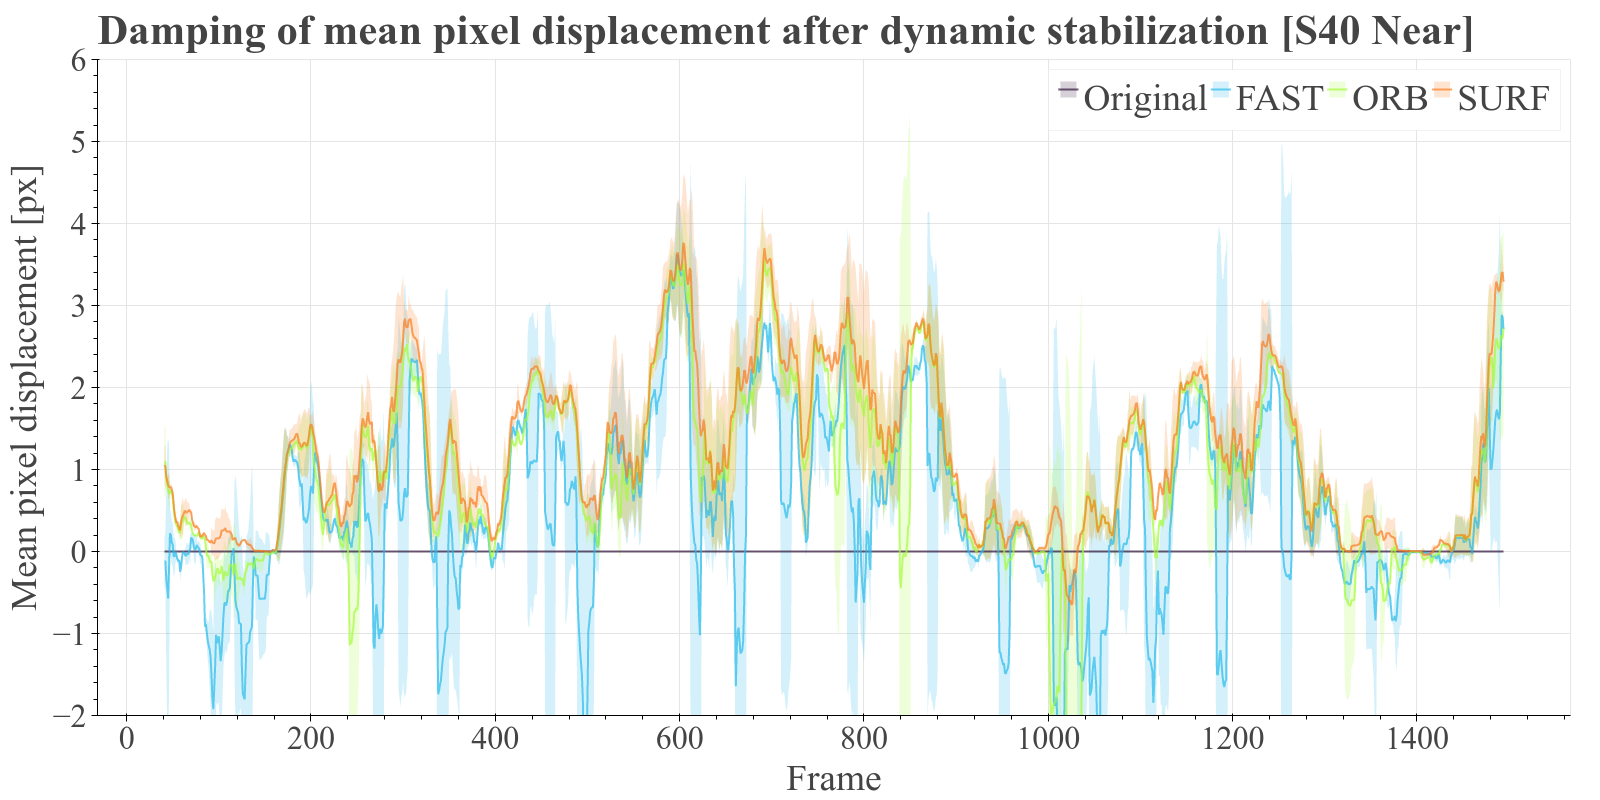
\includegraphics[width=0.475\linewidth]{diagrams/optical_flow/damping_mean_pixel_shifts_after_dynamic_stabilization_s40_near.png}      \\

      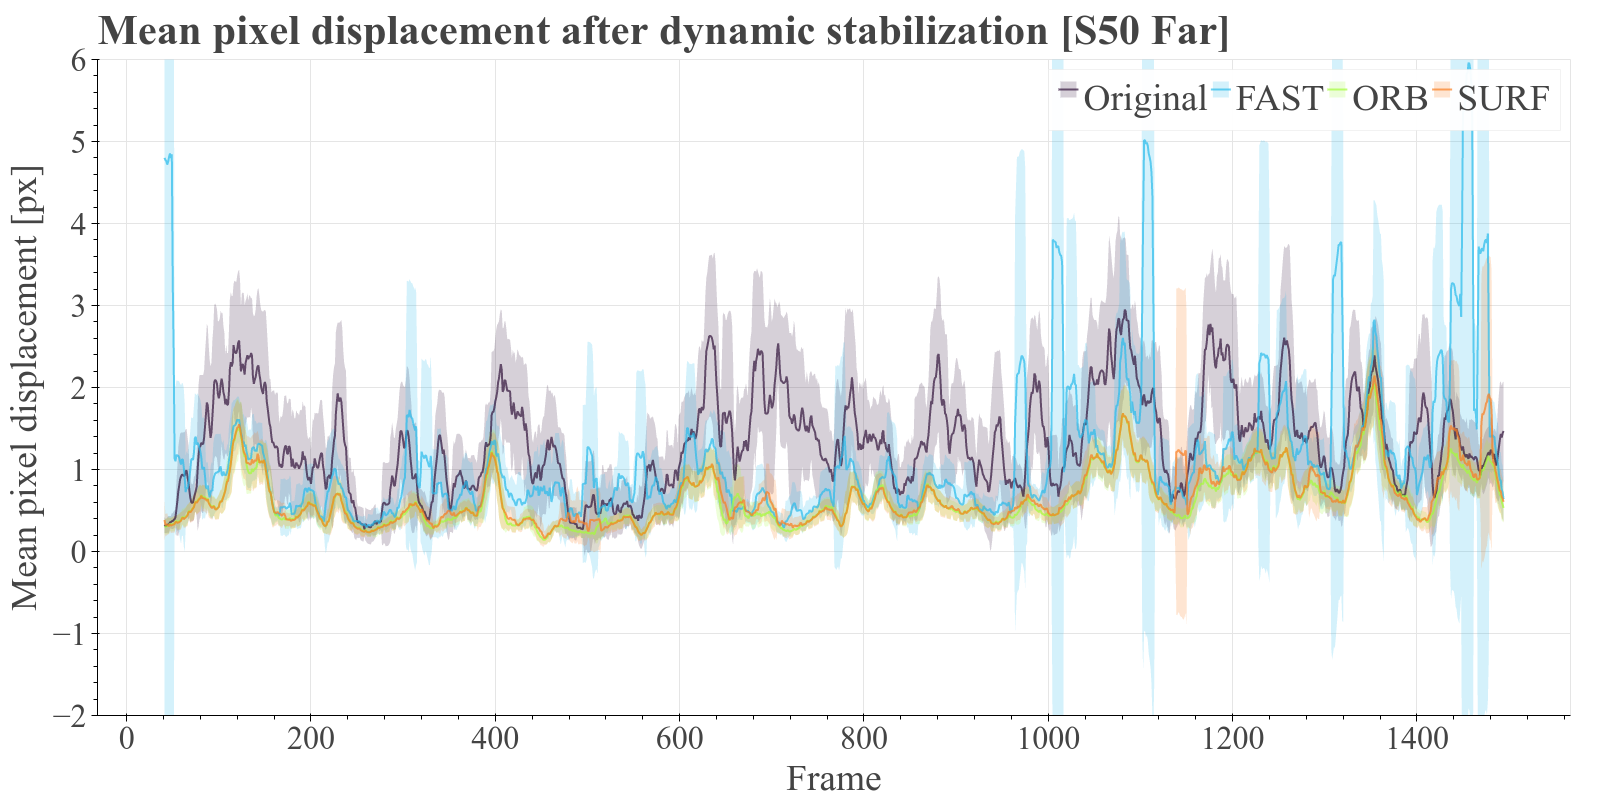
\includegraphics[width=0.475\linewidth]{diagrams/optical_flow/mean_pixel_shifts_after_dynamic_stabilization_s50_far.png}    &  
      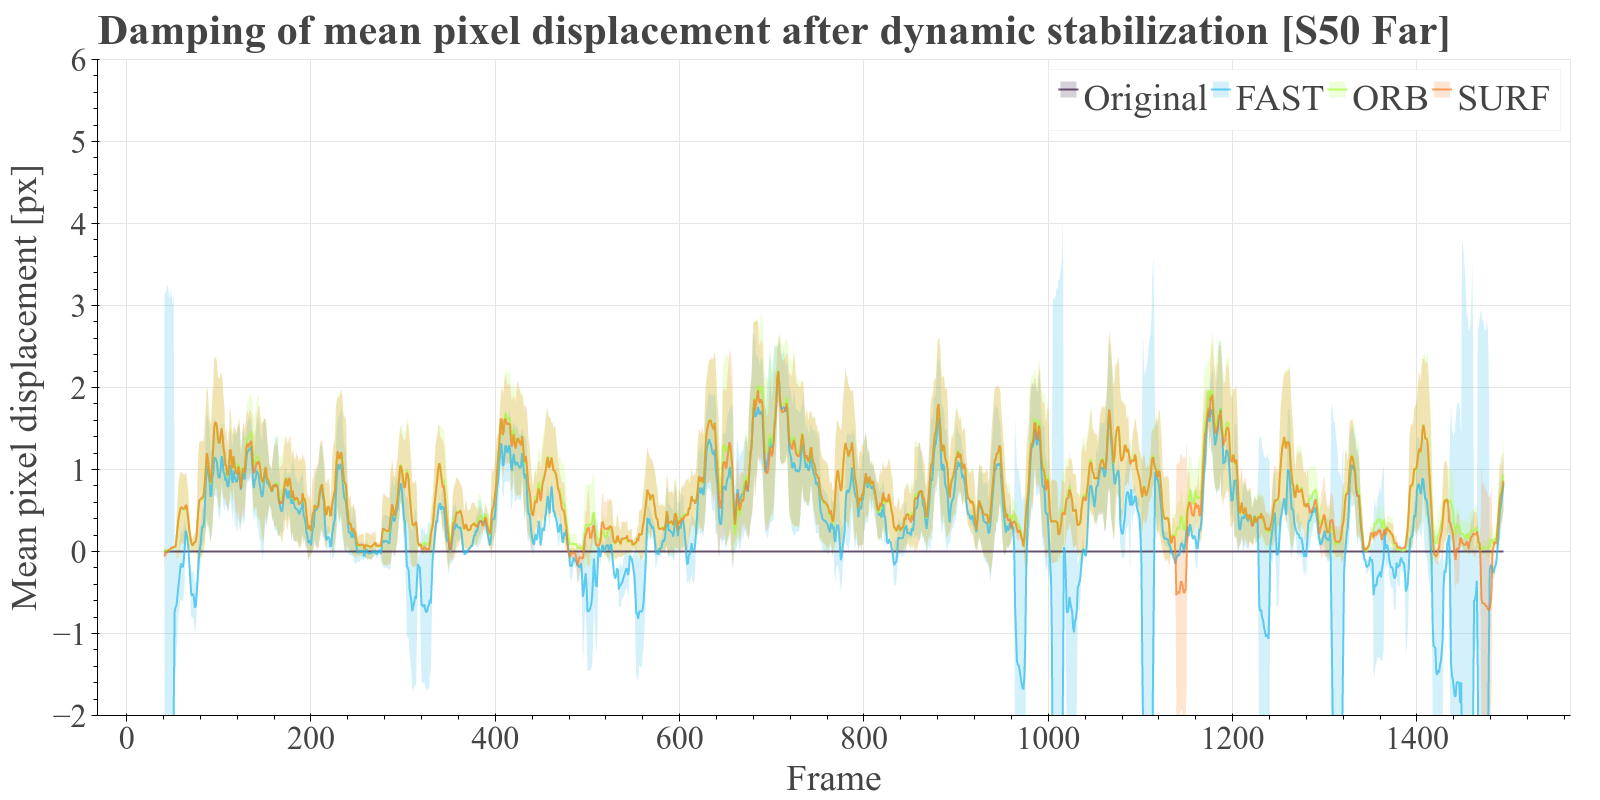
\includegraphics[width=0.475\linewidth]{diagrams/optical_flow/damping_mean_pixel_shifts_after_dynamic_stabilization_s50_far.png}    \\

      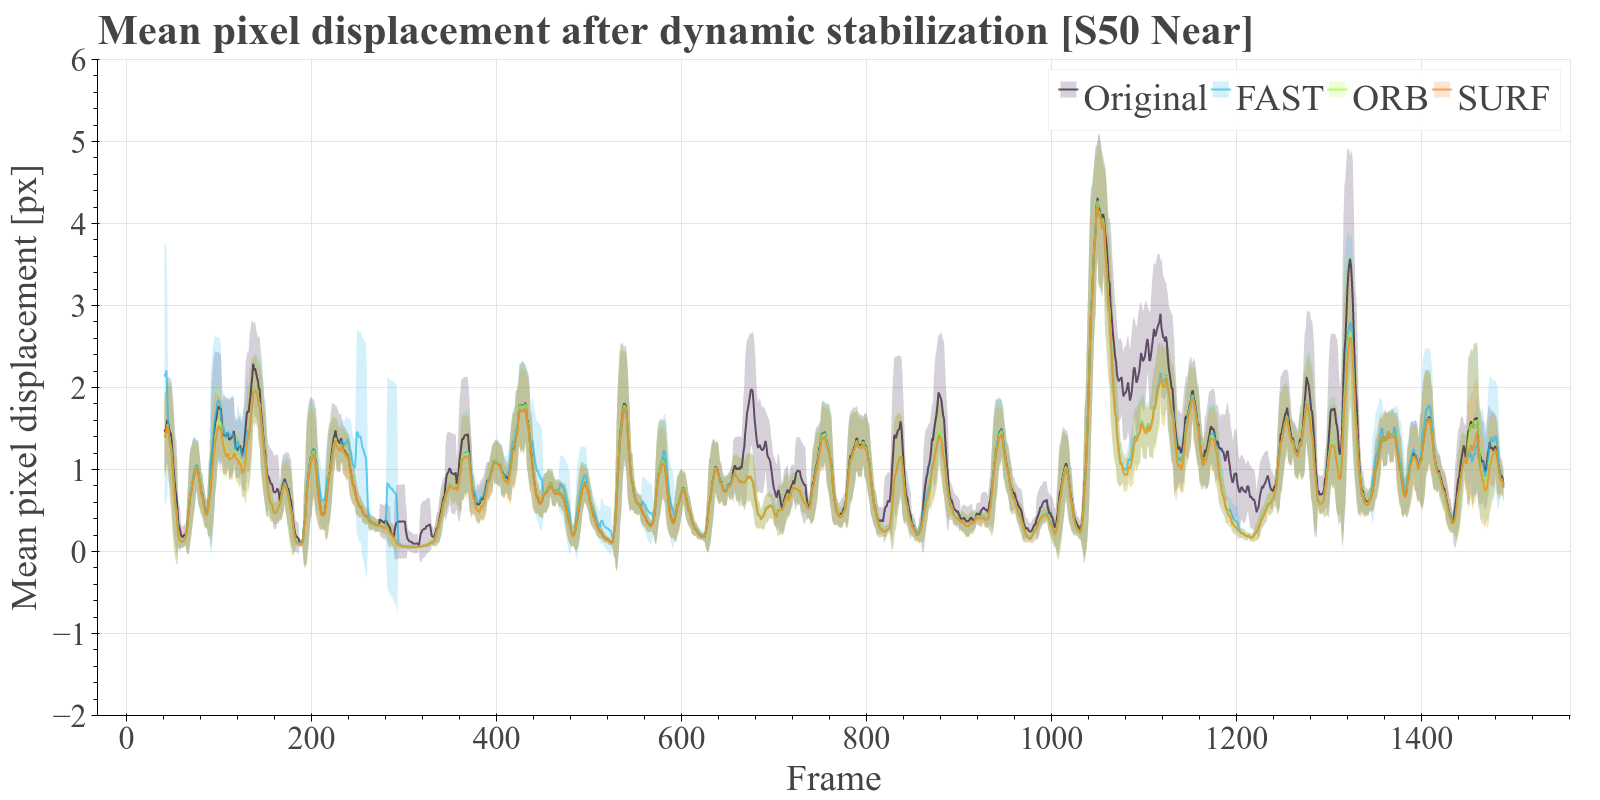
\includegraphics[width=0.475\linewidth]{diagrams/optical_flow/mean_pixel_shifts_after_dynamic_stabilization_s50_near.png}    &  
      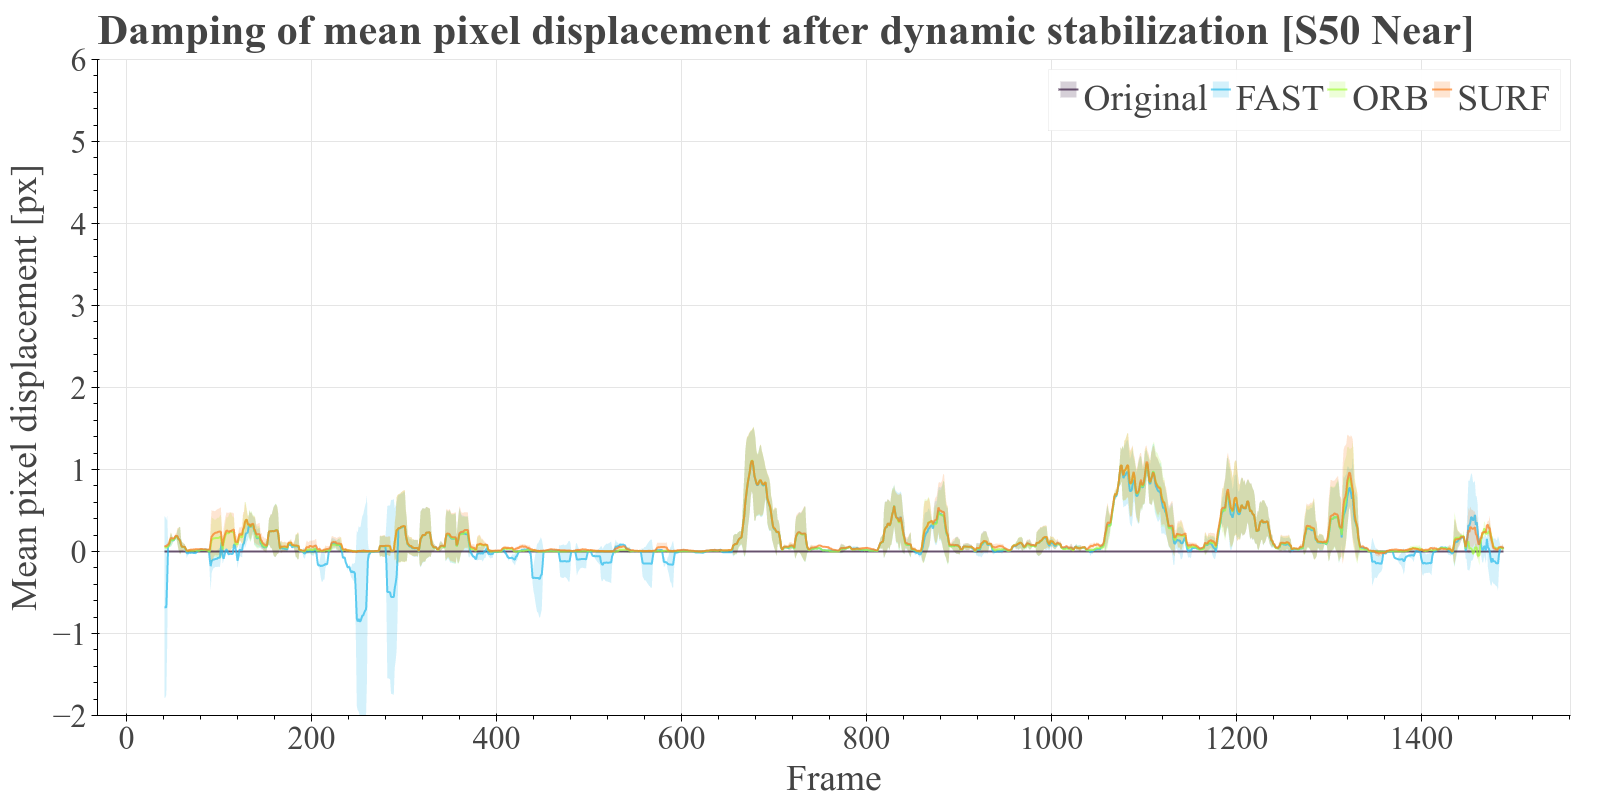
\includegraphics[width=0.475\linewidth]{diagrams/optical_flow/damping_mean_pixel_shifts_after_dynamic_stabilization_s50_near.png}    
    \end{tabular}
    \caption{
        Left: 
        Comparison of the three implemented dynamic stabilizers and the original not stabilized video feed using Optical Flow as metric (lower is better).
        The stabilizers are based on the 
        FAST \cite{Ghahremani_2021,opencv_library} feature detector with FREAK \cite{alahi6247715,opencv_library} feature descriptors,
        SURF \cite{bay10.1007/11744023_32,opencv_library} feature detector and
        ORB \cite{rublee6126544, opencv_library} feature detector.
        The graphs display the mean pixel shift at each frame. 
        Right: 
        The damping capabilities of the same three stabilizers (higher is better). 
        The graphs approximate the removed jitter in the mean pixel shift between the original video and the stabilizer at each frame.\\
        For visualization the values are filtered using the rolling mean over 12 frames. 
        The light areas display the standard deviation within the window.
    }
    \label{fig:dynamic_stabilization_appendix}
    \end{figure*}

    

\begin{table}[!h]
    \centering
    \begin{tabular}{ |l|l|r|r|r| } 
     \hline
     \textbf{Stabilizer} & \textbf{Camera} & \textbf{Disp.}  & \textbf{Better} & \textbf{Better [\%]} \\ 
     \hline
     Original   & \camsf{4} & 3.515 & 0     &  0.0      \\
     FAST       & \camsf{4} & 1.999 & 1279  &  85.552   \\
     ORB        & \camsf{4} & 1.632 & 1396  &  93.378   \\
     SURF       & \camsf{4} & 1.273 & 1478  &  \textbf{98.863}   \\
     \hline

     Original   & \camsn{4} & 5.084 & 0     &  0.0      \\
     FAST       & \camsn{4} & 4.371 & 983   &  65.753   \\
     ORB        & \camsn{4} & 4.222 & 1024  &  68.495   \\
     SURF       & \camsn{4} & 2.495 & 1403  &  \textbf{93.846}   \\
     \hline

     Original   & \camsf{5} & 2.624 & 0  &    0.0    \\
     FAST       & \camsf{5} & 2.749 & 983  &  65.753   \\
     ORB        & \camsf{5} & 1.510 & 1258  & 84.147    \\
     SURF       & \camsf{5} & 1.550 & 1273  & \textbf{85.151}    \\
     \hline

     Original   & \camsn{5} & 2.212 &   0   &  0.0      \\
     FAST       & \camsn{5} & 1.847 & 1028   &  68.993   \\
     ORB        & \camsn{5} & 1.671 &  1234 &    82.819 \\
     SURF       & \camsn{5} & 1.543 & 1290  &   \textbf{86.577}  \\
     \hline
    \end{tabular}
    \caption{
            Comparison of the implemented dynamic stabilizers and the original not stabilized video feed using Optical Flow as metric.
            It shows that most of the stabilizers exhibit a lower mean displacement (Disp.) after dynamic stabilization. 
            In terms of the number of frames the stabilizers all show a high number of total (Better) and relative (Better \%) frames where they have a lower mean displacement. 
            Especially for the SURF \cite{bay10.1007/11744023_32,opencv_library} feature detector (bold) the improvement is substantially.
        }
    \label{tab:dynamic_stabilization}
\end{table}



\begin{figure*}[!ht]
  \centering
  \begin{tabular}{cc}
    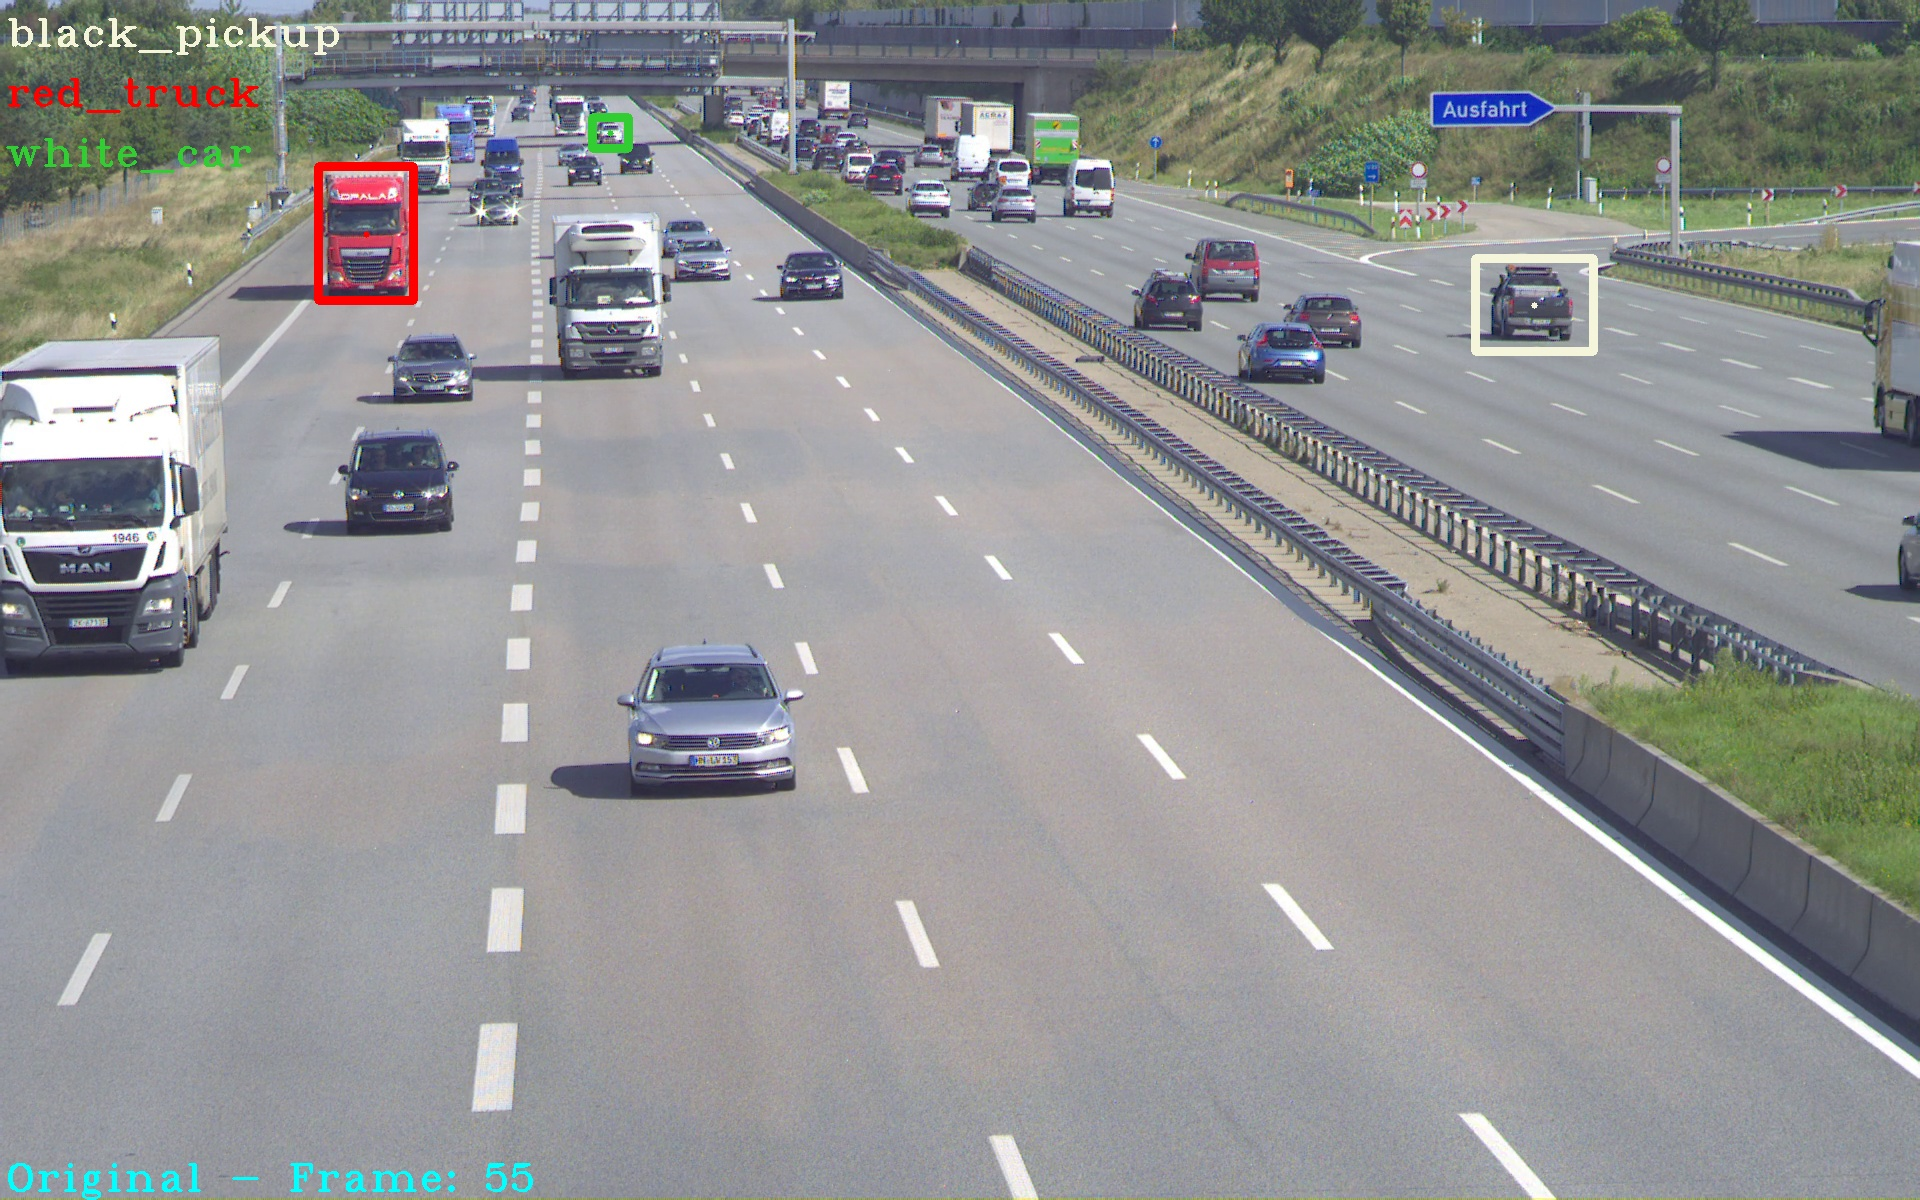
\includegraphics[width=0.45\linewidth]{diagrams/object_tracking/s40_n_far/frame.png}    &  
    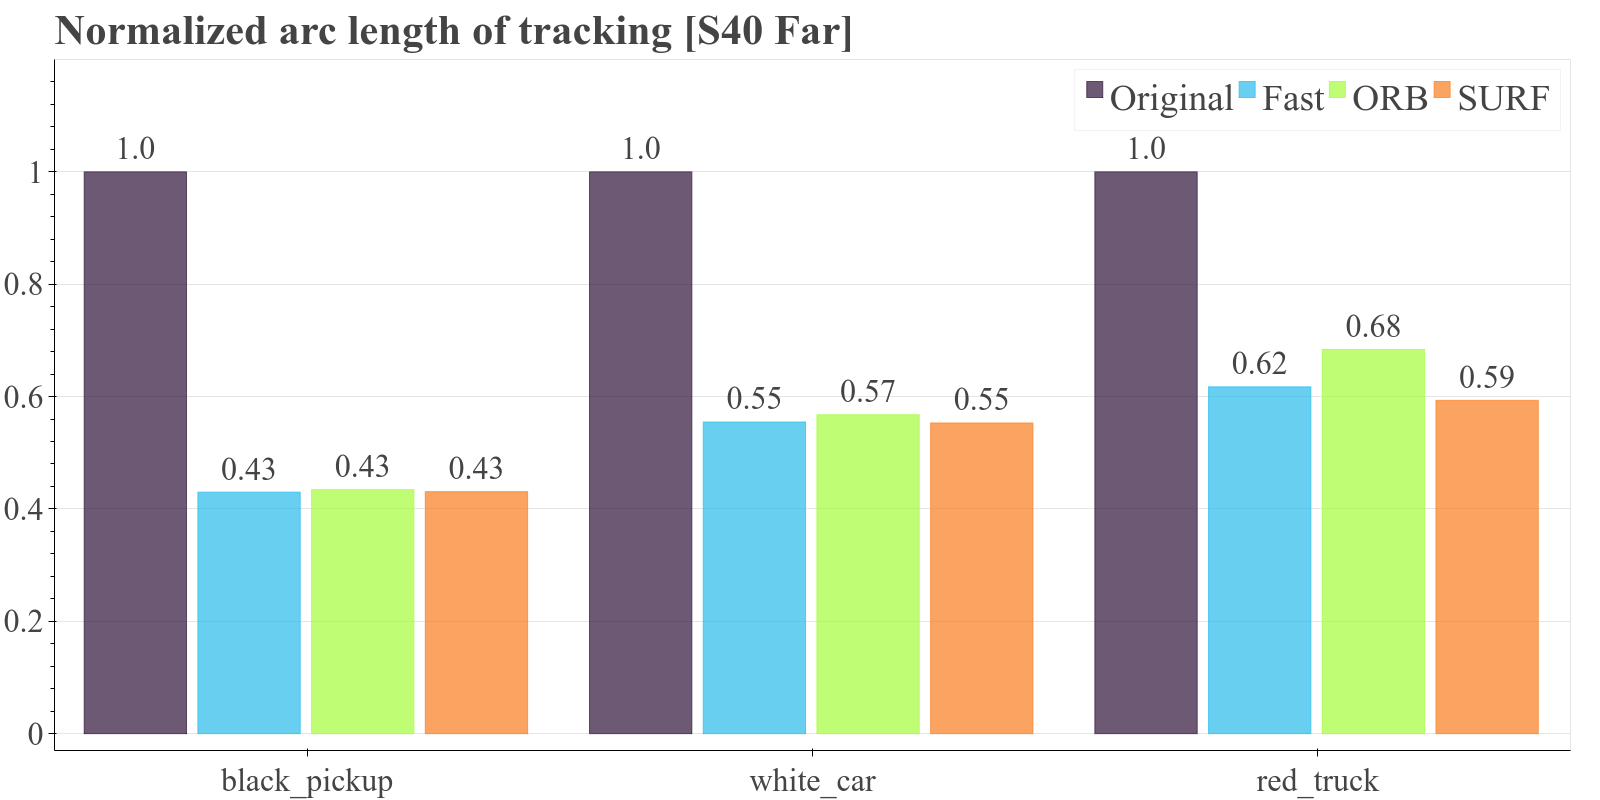
\includegraphics[width=0.475\linewidth]{diagrams/object_tracking/s40_n_far/arcs.png}    \\

    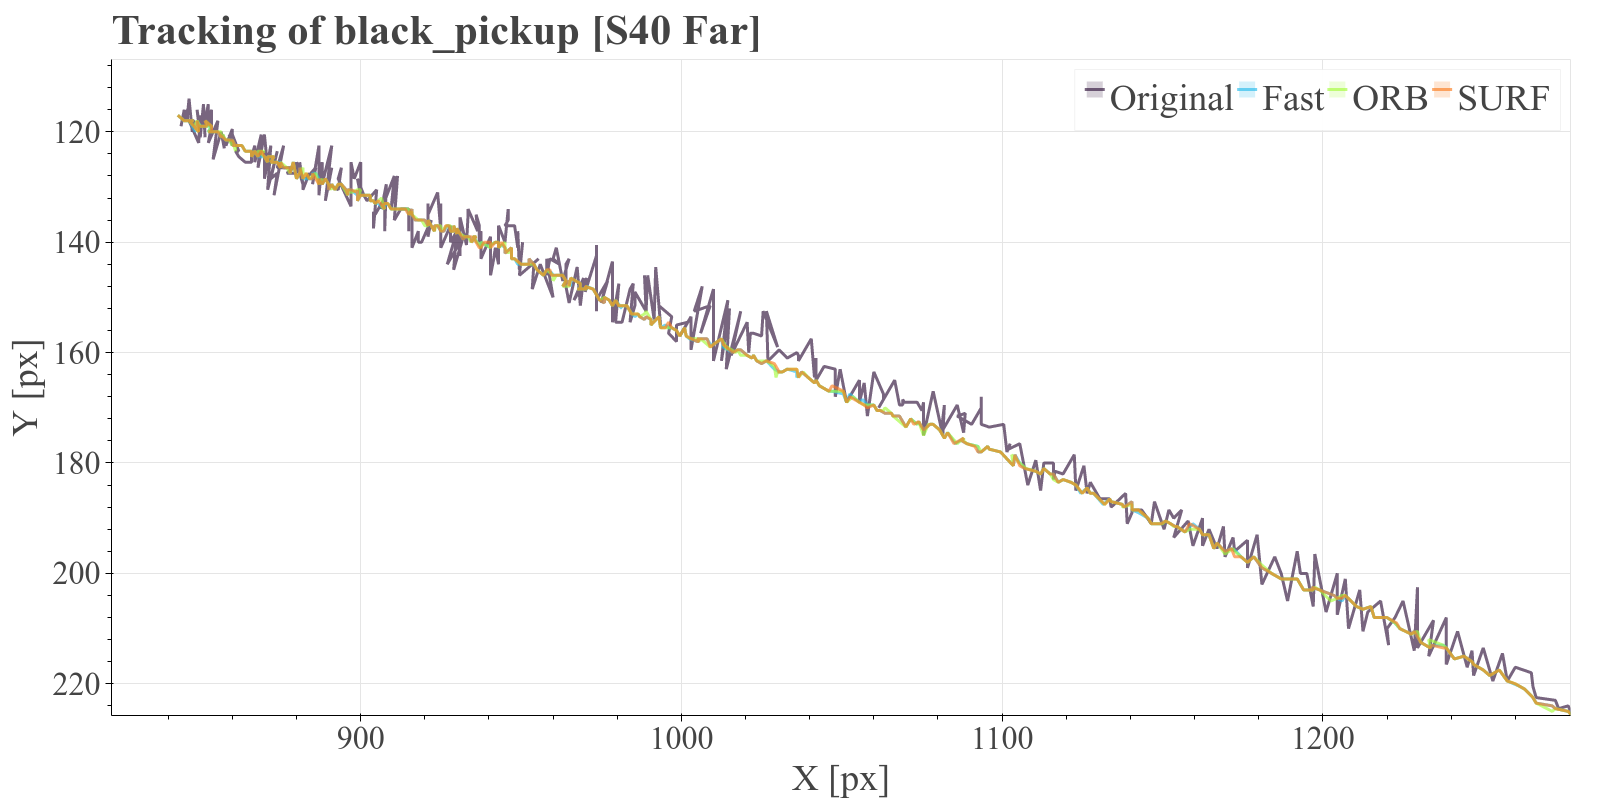
\includegraphics[width=0.475\linewidth]{diagrams/object_tracking/s40_n_far/black_pickup.png}    &  
    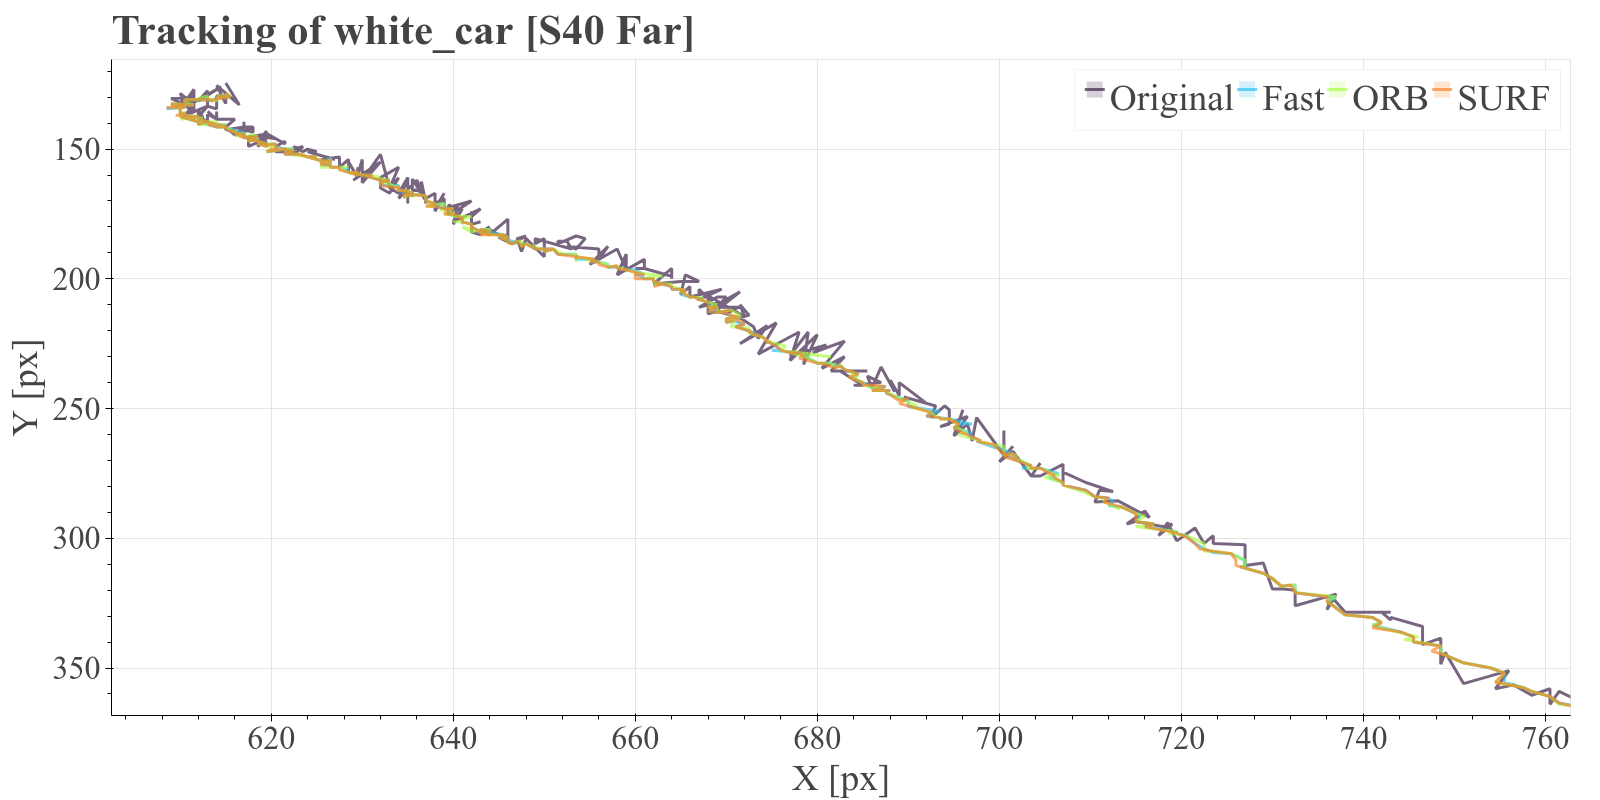
\includegraphics[width=0.475\linewidth]{diagrams/object_tracking/s40_n_far/white_car.png}    \\  
    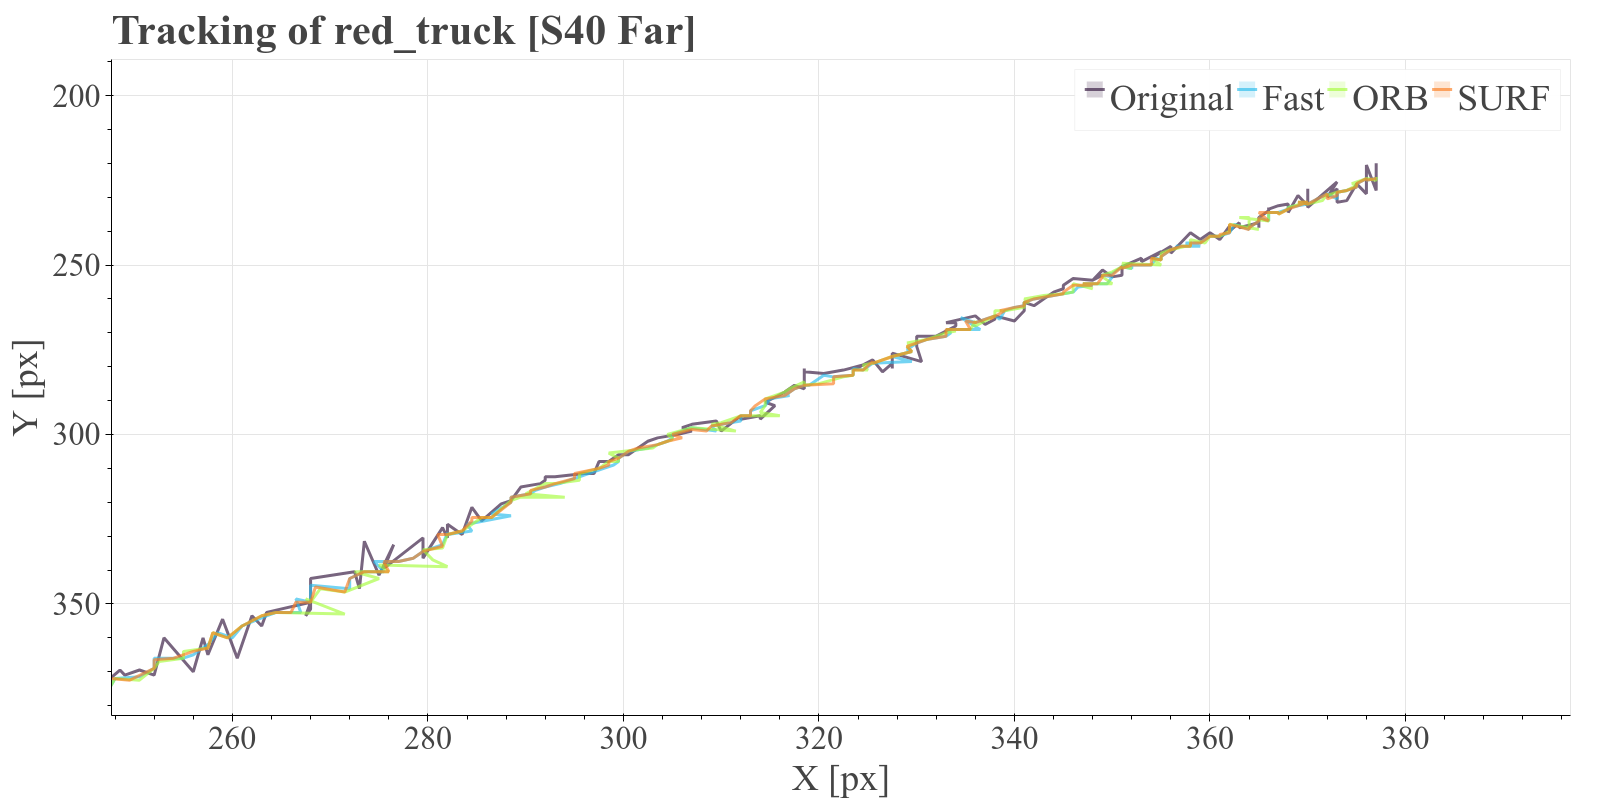
\includegraphics[width=0.475\linewidth]{diagrams/object_tracking/s40_n_far/red_truck.png}   
  \end{tabular}
  \caption{Left: 
  The exemplary vehicles tracked through the video sequence of the camera \camsn{4}. 
  Right:
  The corresponding normalized arc lengths of the pixel path. 
  The length is normalized by the original arc length, hence the 1.0 factor for the original video. 
  As the jitter is removed, the pixels movement is lowered significantly as it does only move with the vehicle, not the camera.
  This can be seen with around half of the path length remaining after stabilization for all stabilizers.
  }
  \label{fig:object_tracking_appendix_s40_n_far}
\end{figure*}



\begin{figure*}[!ht]
  \centering
  \begin{tabular}{cc}
    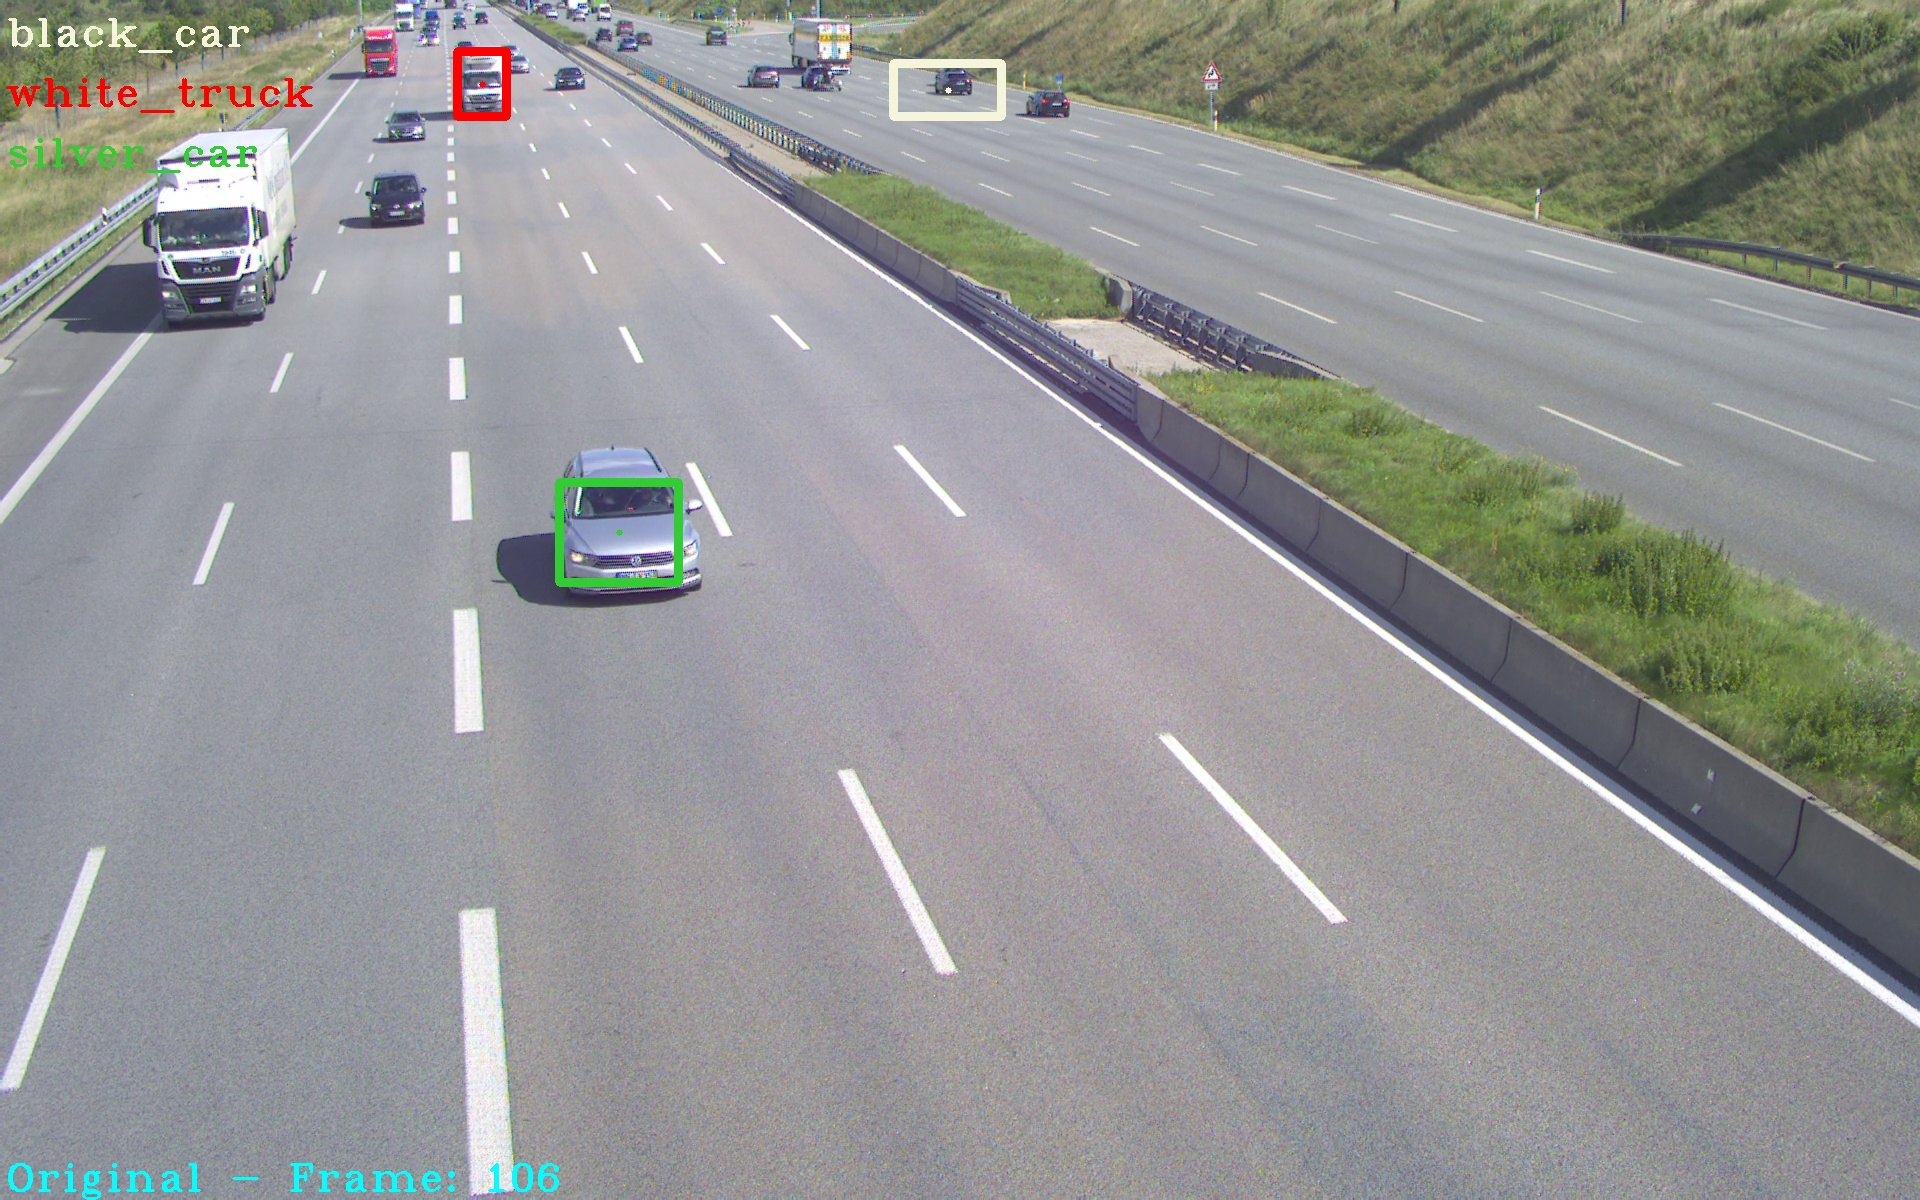
\includegraphics[width=0.45\linewidth]{diagrams/object_tracking/s40_n_near/frame.png}    &  
    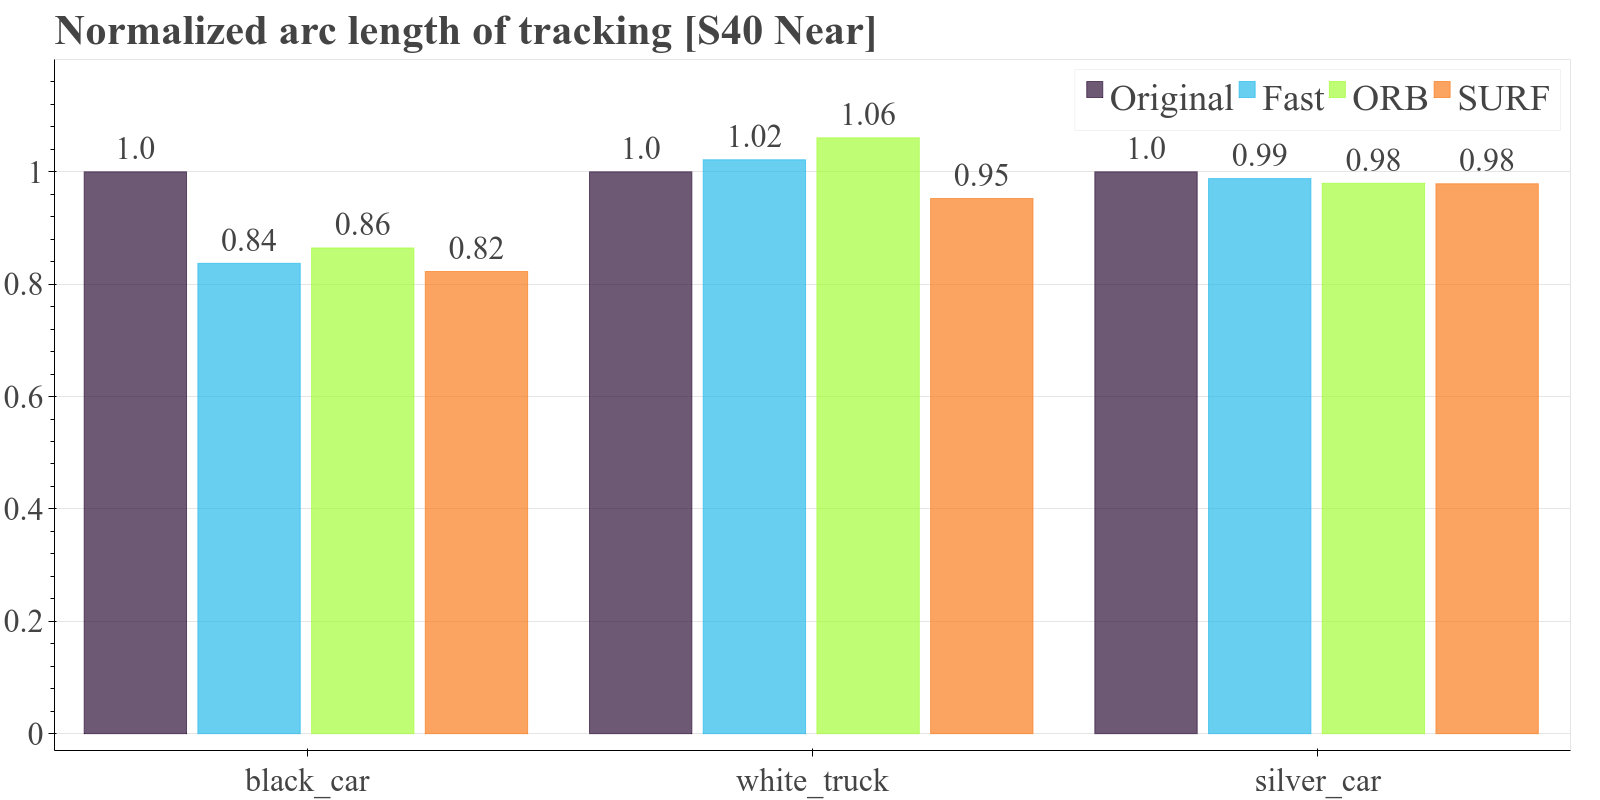
\includegraphics[width=0.475\linewidth]{diagrams/object_tracking/s40_n_near/arcs.png}    \\

    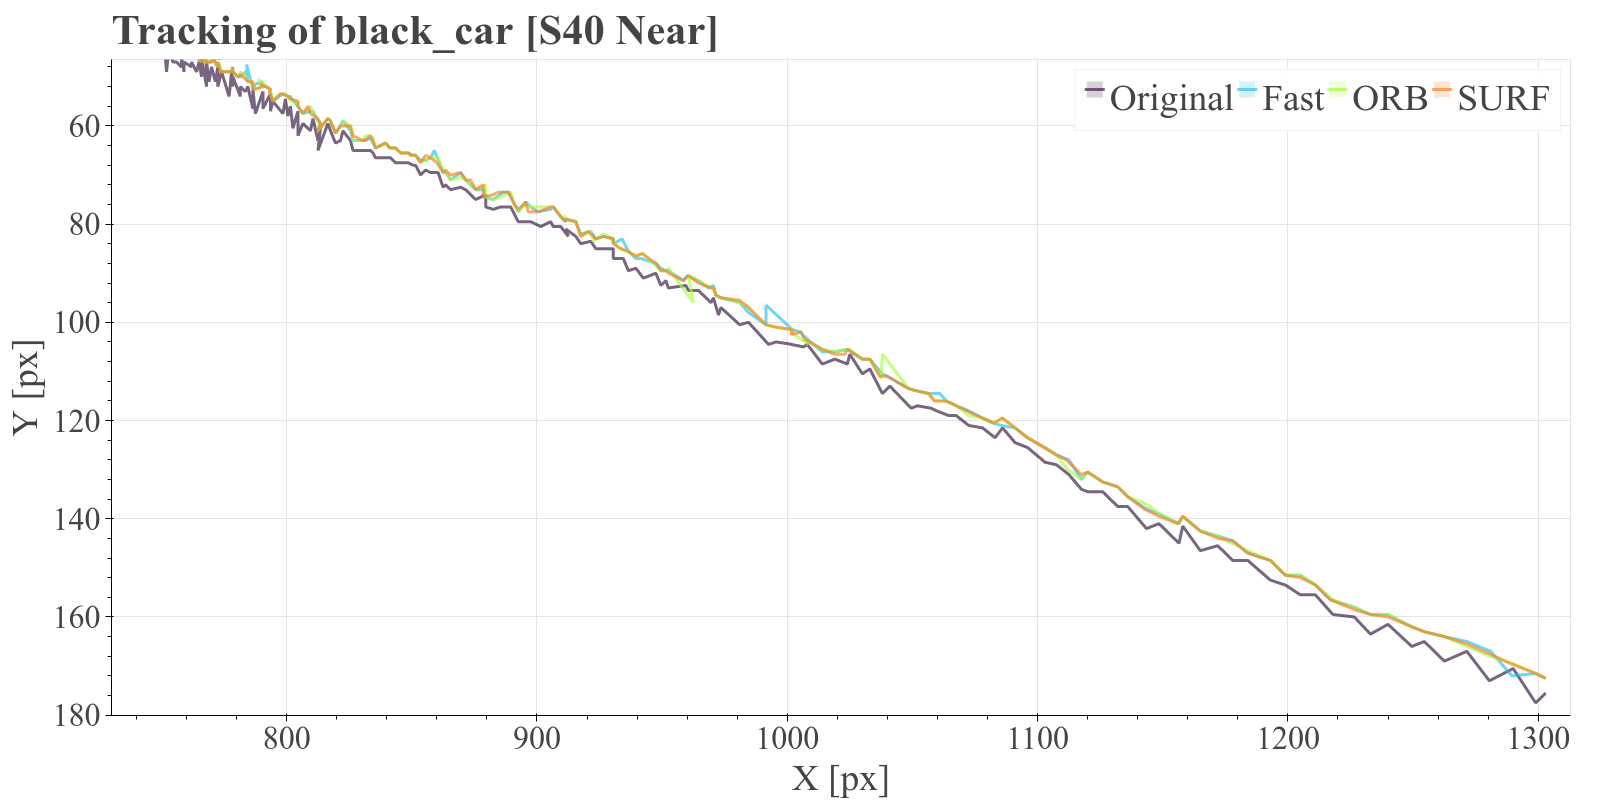
\includegraphics[width=0.475\linewidth]{diagrams/object_tracking/s40_n_near/black_car.png}    &  
    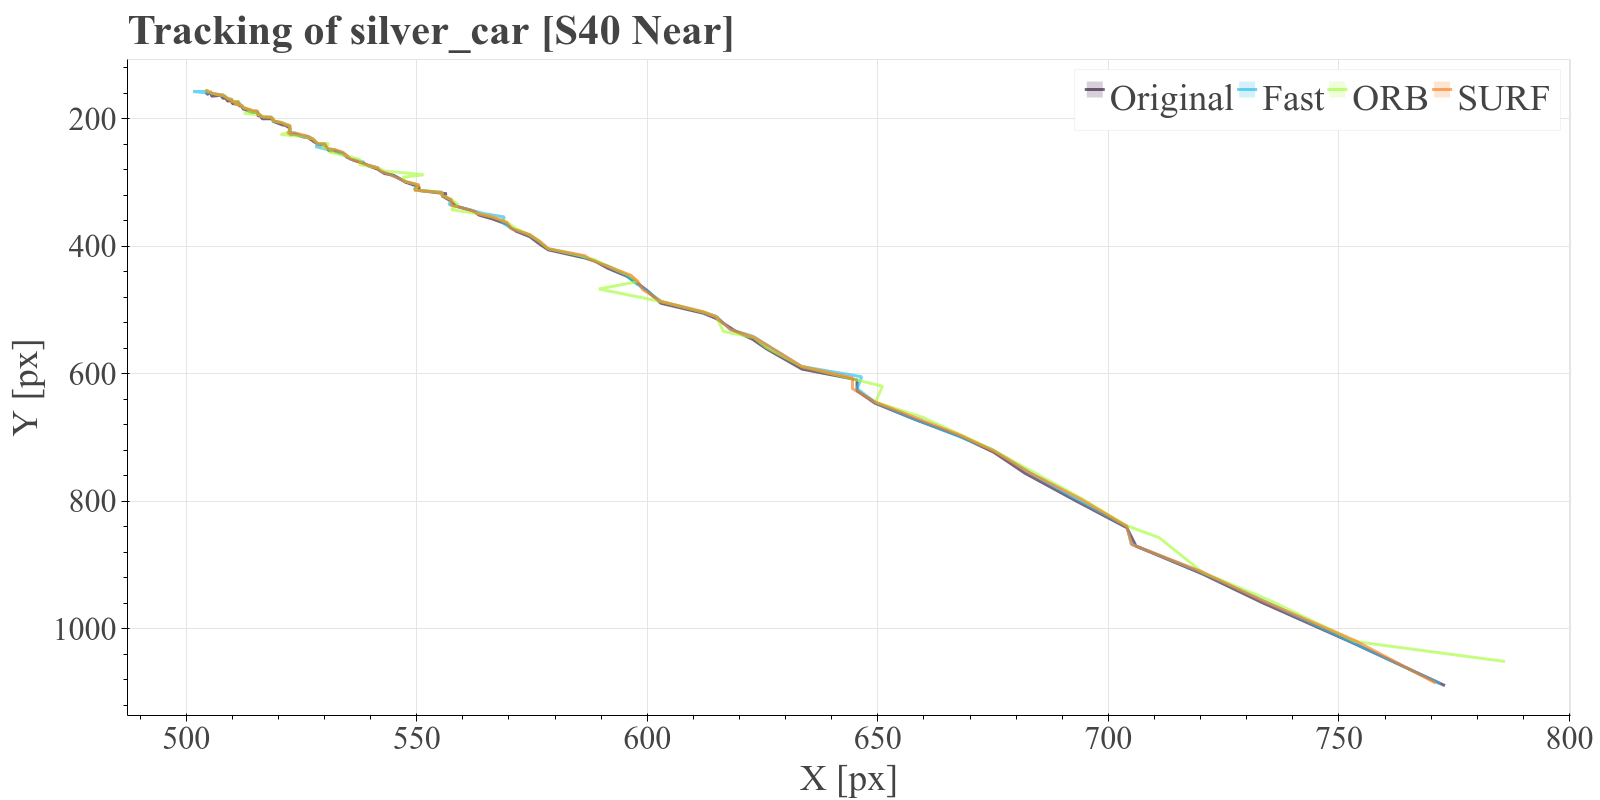
\includegraphics[width=0.475\linewidth]{diagrams/object_tracking/s40_n_near/silver_car.png}    \\  
    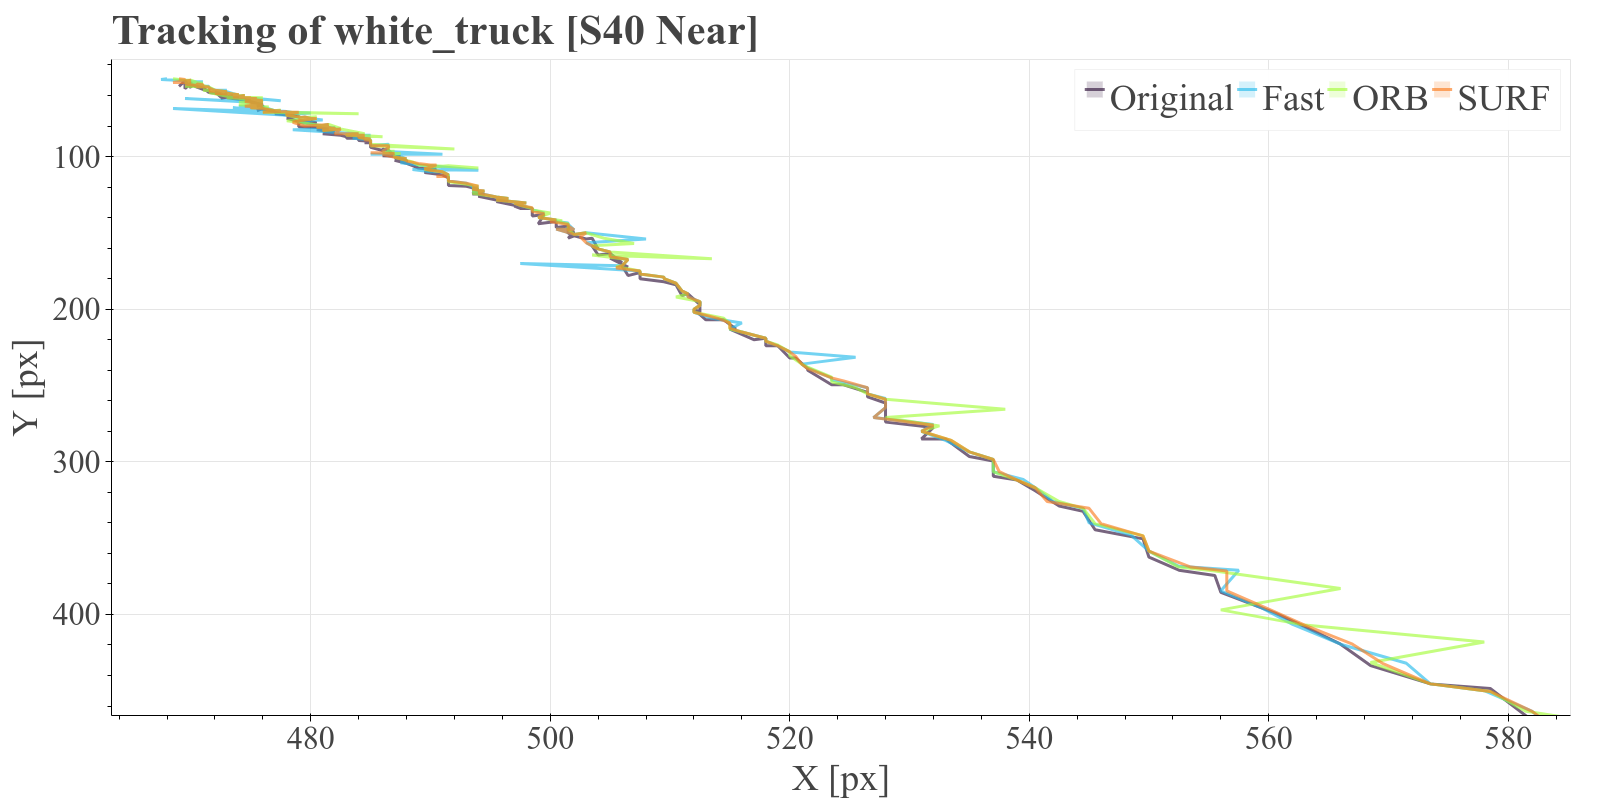
\includegraphics[width=0.475\linewidth]{diagrams/object_tracking/s40_n_near/white_truck.png}   
  \end{tabular}
  \caption{Left: 
  The exemplary vehicles tracked through the video sequence of the camera \camsn{4}. 
  Right:
  The corresponding normalized arc lengths of the pixel path. 
  The length is normalized by the original arc length, hence the 1.0 factor for the original video. 
  As the jitter is removed, the pixels movement is lowered significantly as it does only move with the vehicle, not the camera.
  This can be seen with around half of the path length remaining after stabilization for all stabilizers.
  }
  \label{fig:object_tracking_appendix_s40_n_near}
\end{figure*}



\begin{figure*}[!ht]
  \centering
  \begin{tabular}{cc}
    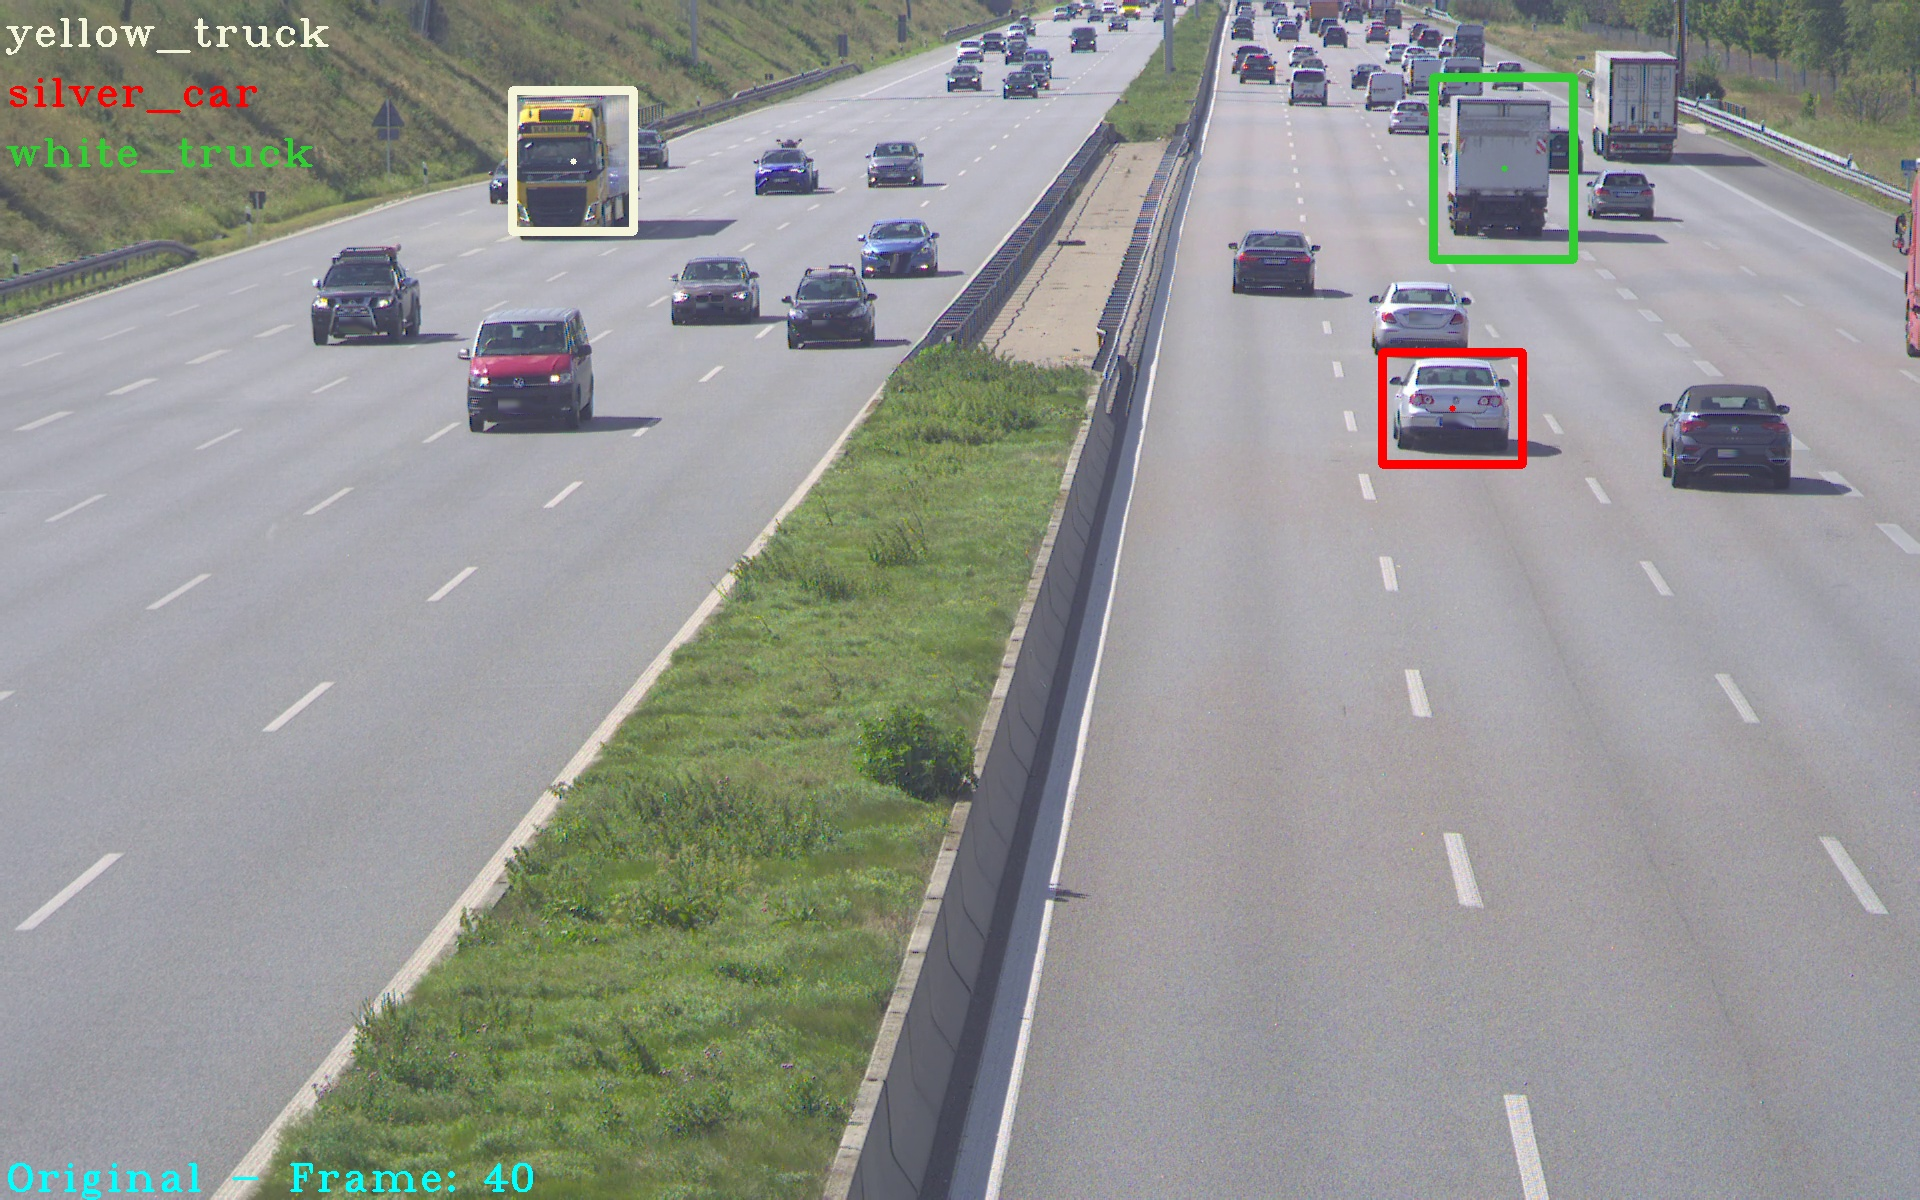
\includegraphics[width=0.45\linewidth]{diagrams/object_tracking/s50_s_far/frame.png}    &  
    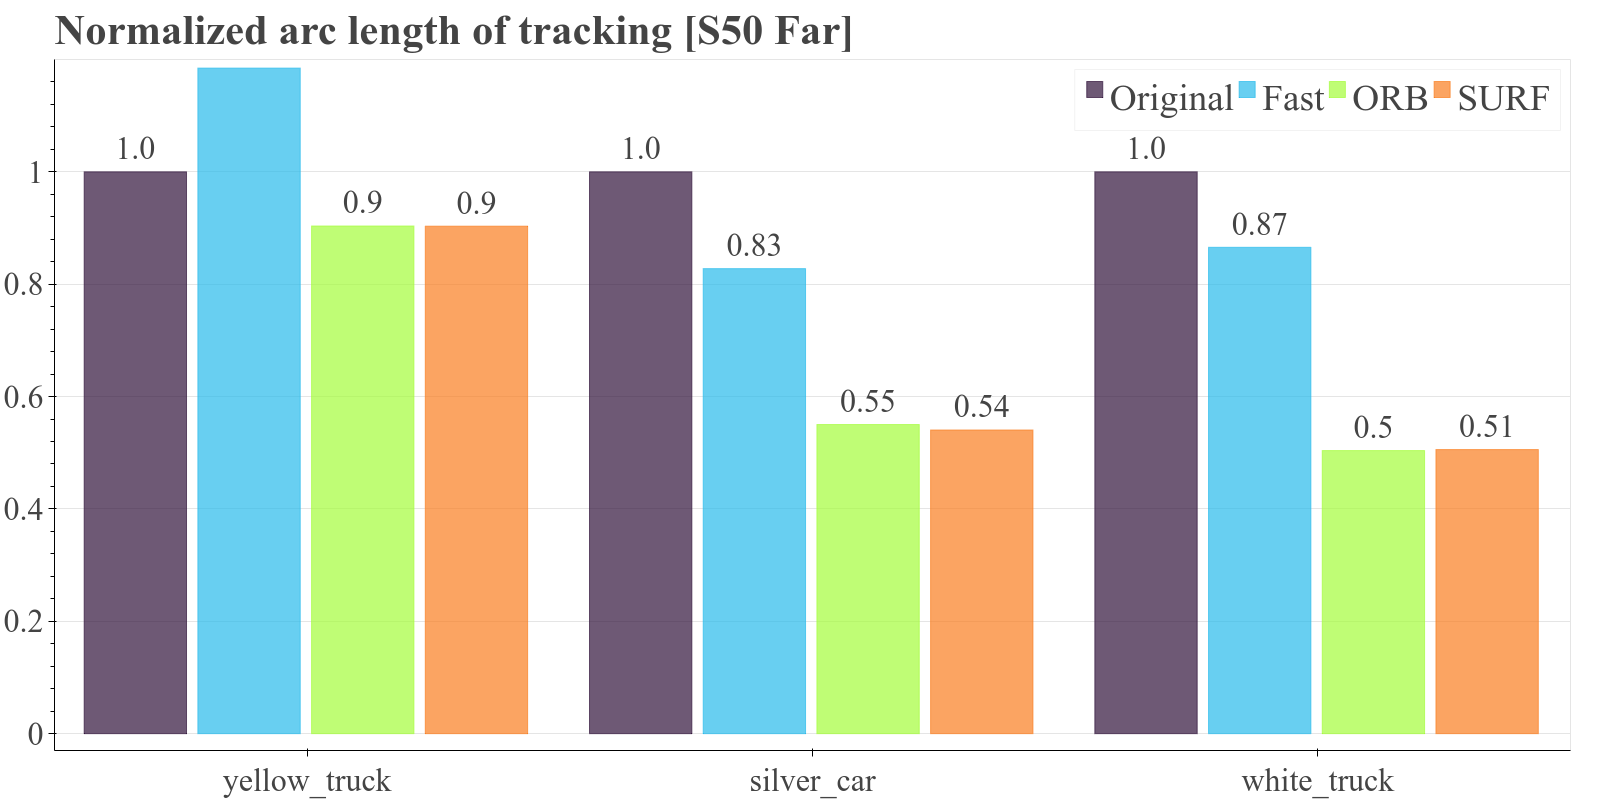
\includegraphics[width=0.475\linewidth]{diagrams/object_tracking/s50_s_far/arcs.png}    \\

    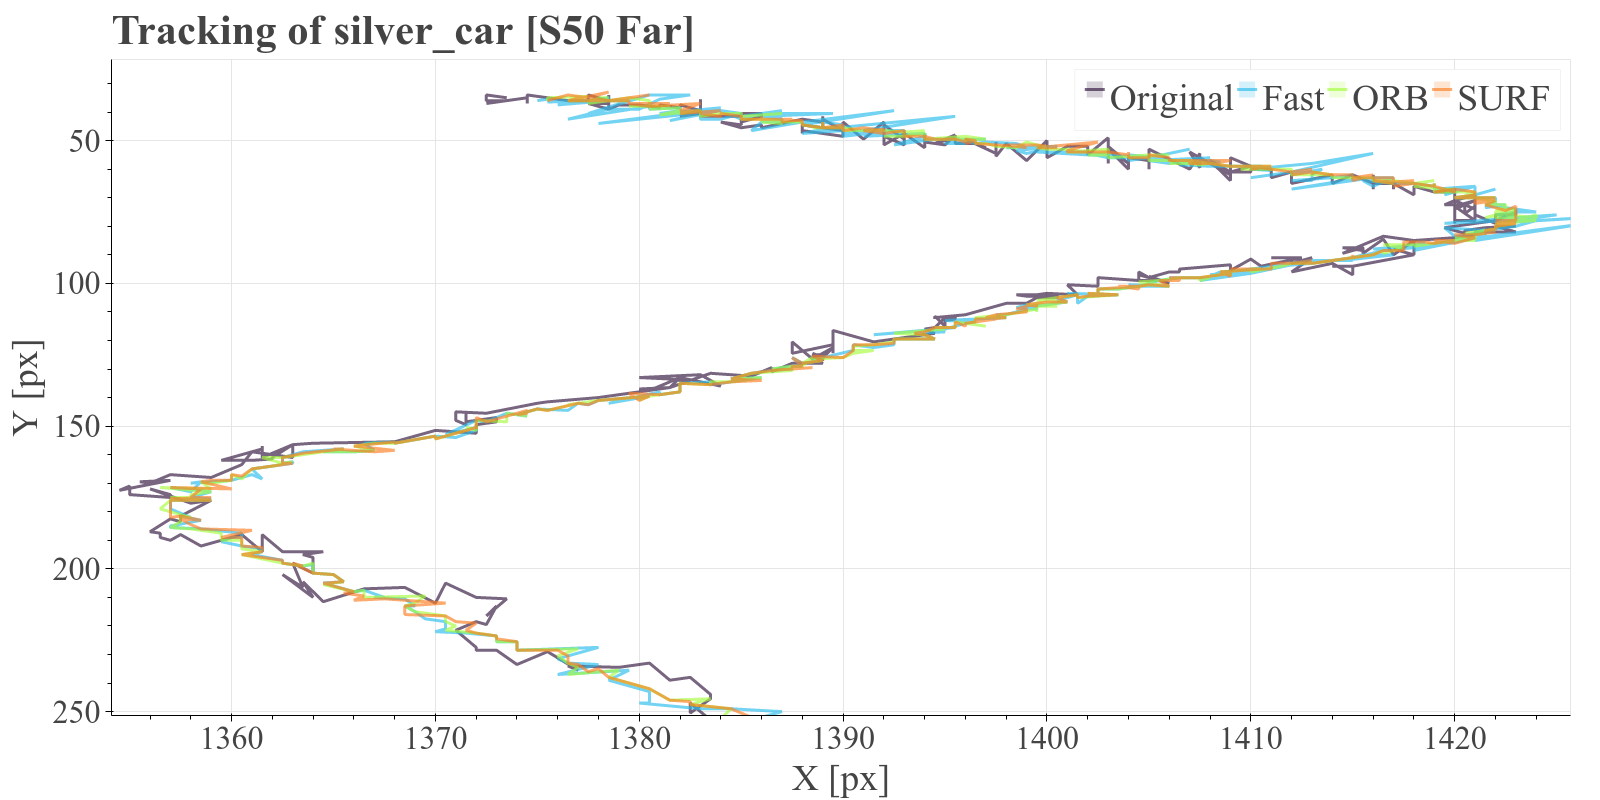
\includegraphics[width=0.475\linewidth]{diagrams/object_tracking/s50_s_far/silver_car.png}    &  
    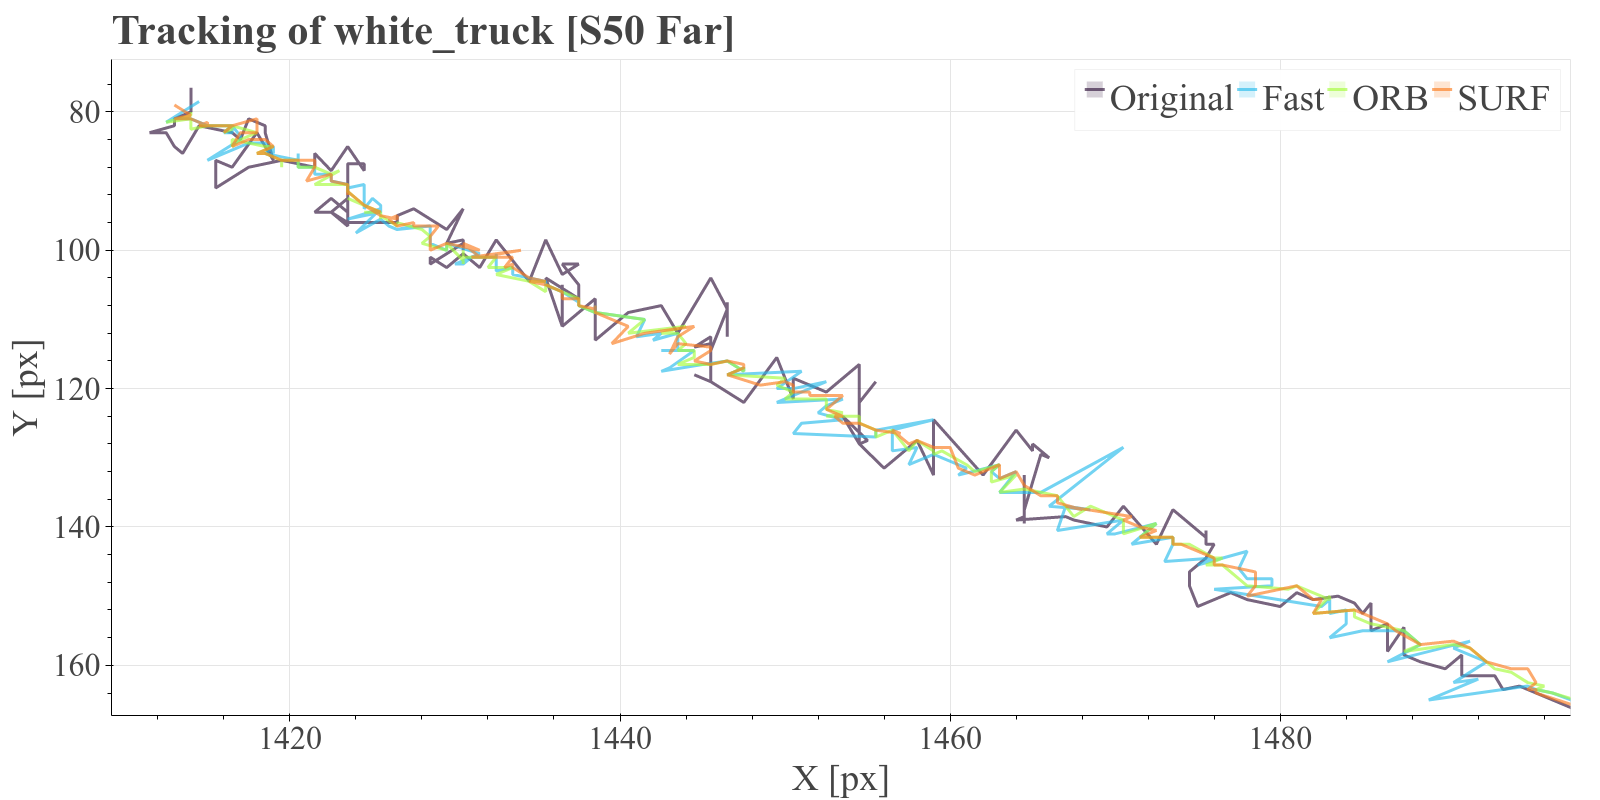
\includegraphics[width=0.475\linewidth]{diagrams/object_tracking/s50_s_far/white_truck.png}    \\  
    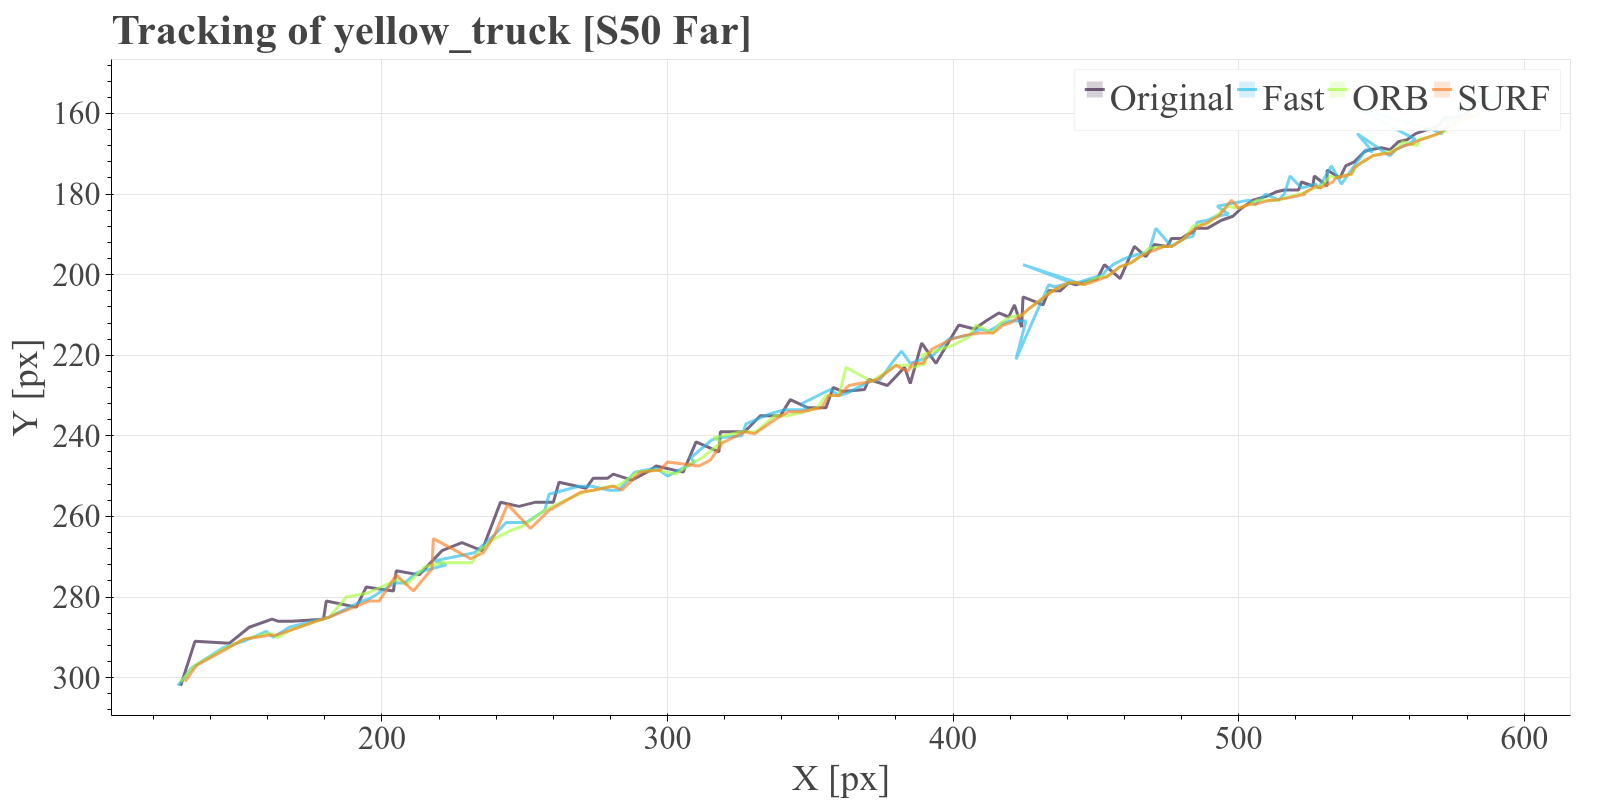
\includegraphics[width=0.475\linewidth]{diagrams/object_tracking/s50_s_far/yellow_truck.png}   
  \end{tabular}
  \caption{Left: 
  The exemplary vehicles tracked through the video sequence of the camera \camsn{4}. 
  Right:
  The corresponding normalized arc lengths of the pixel path. 
  The length is normalized by the original arc length, hence the 1.0 factor for the original video. 
  As the jitter is removed, the pixels movement is lowered significantly as it does only move with the vehicle, not the camera.
  This can be seen with around half of the path length remaining after stabilization for all stabilizers.
  }
  \label{fig:object_tracking_appendix_s50_s_far}
\end{figure*}



\begin{figure*}[!ht]
  \centering
  \begin{tabular}{cc}
    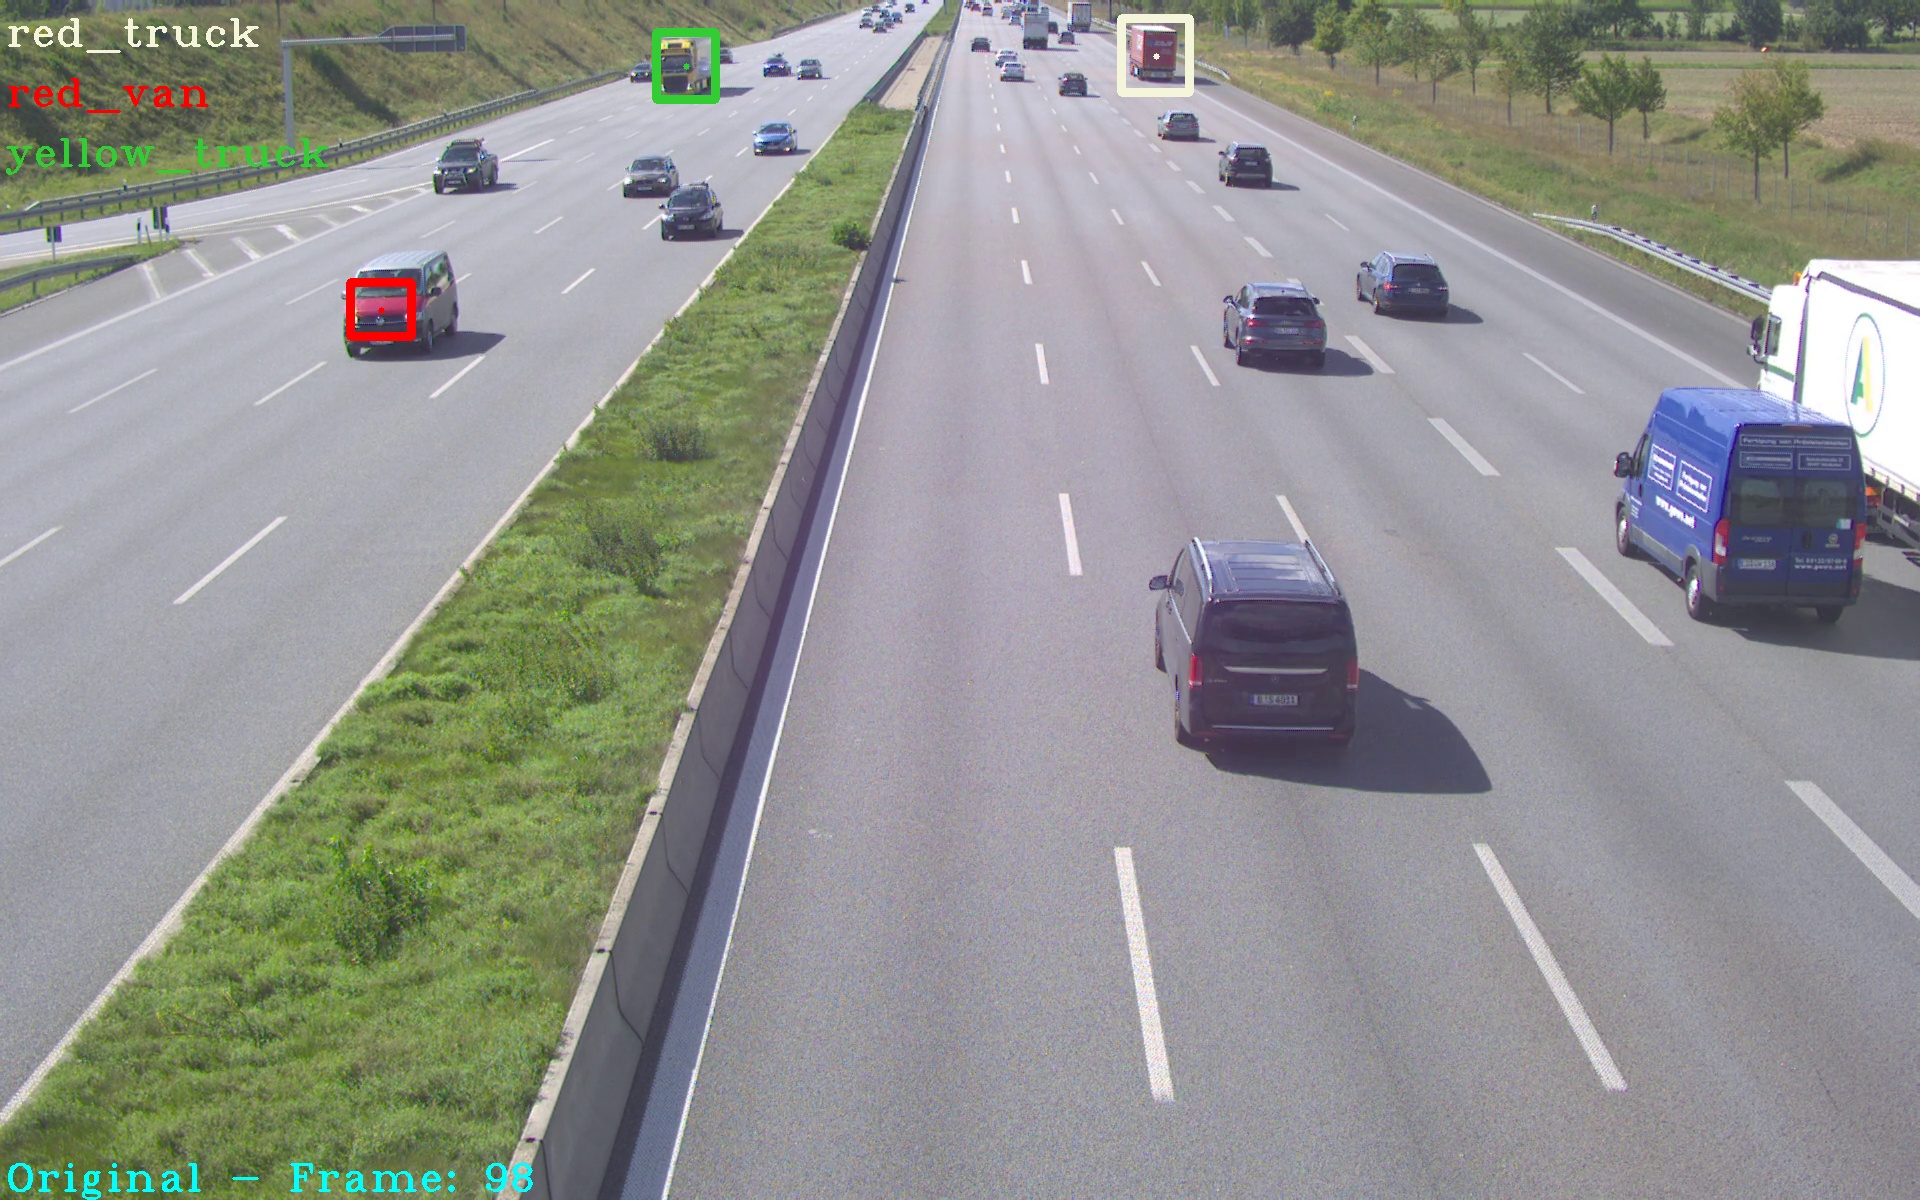
\includegraphics[width=0.45\linewidth]{diagrams/object_tracking/s50_s_near/frame.png}    &  
    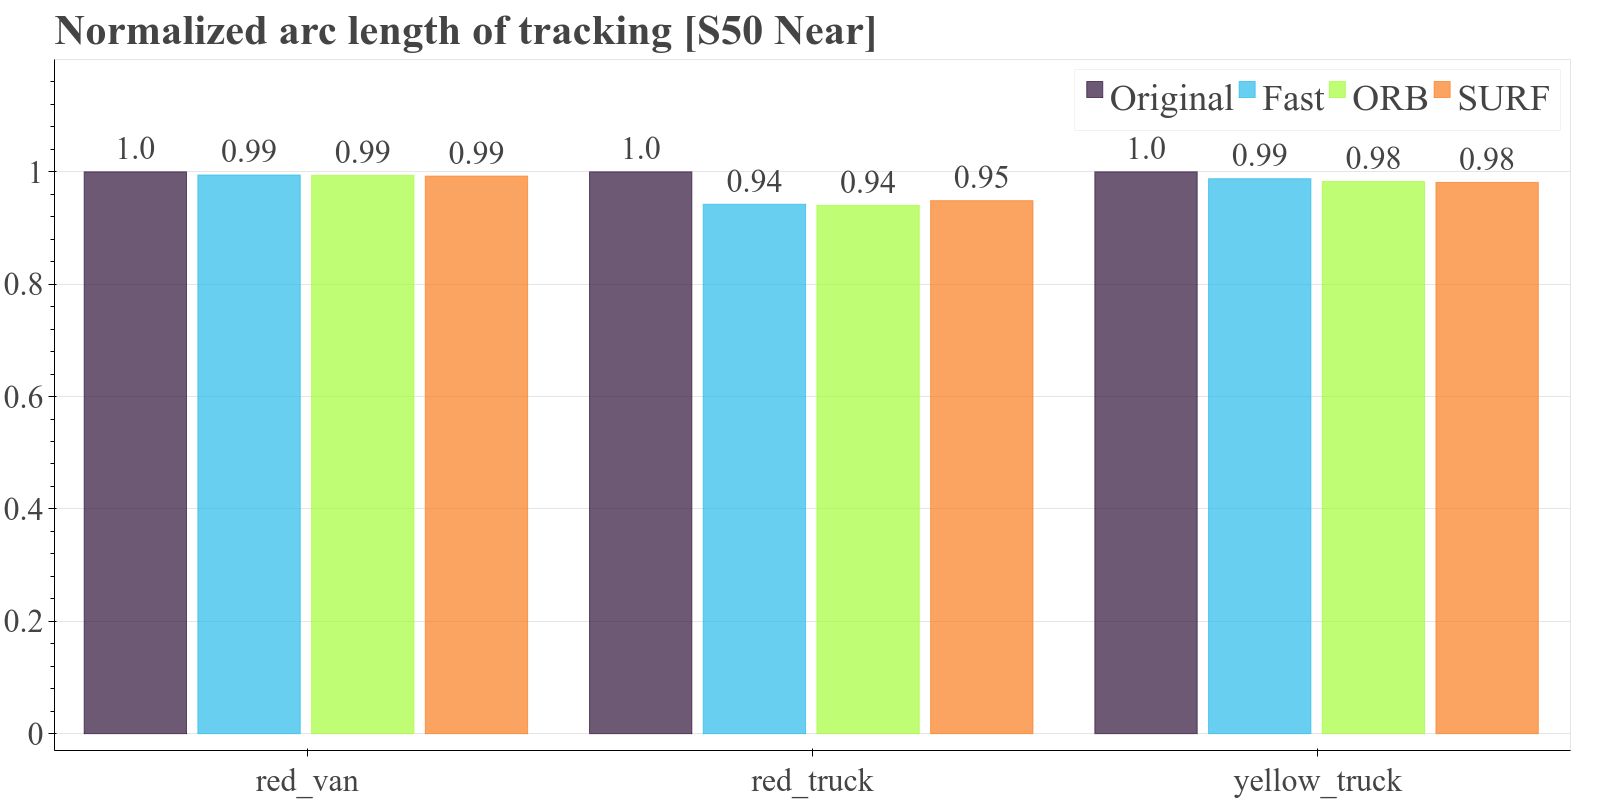
\includegraphics[width=0.475\linewidth]{diagrams/object_tracking/s50_s_near/arcs.png}    \\

    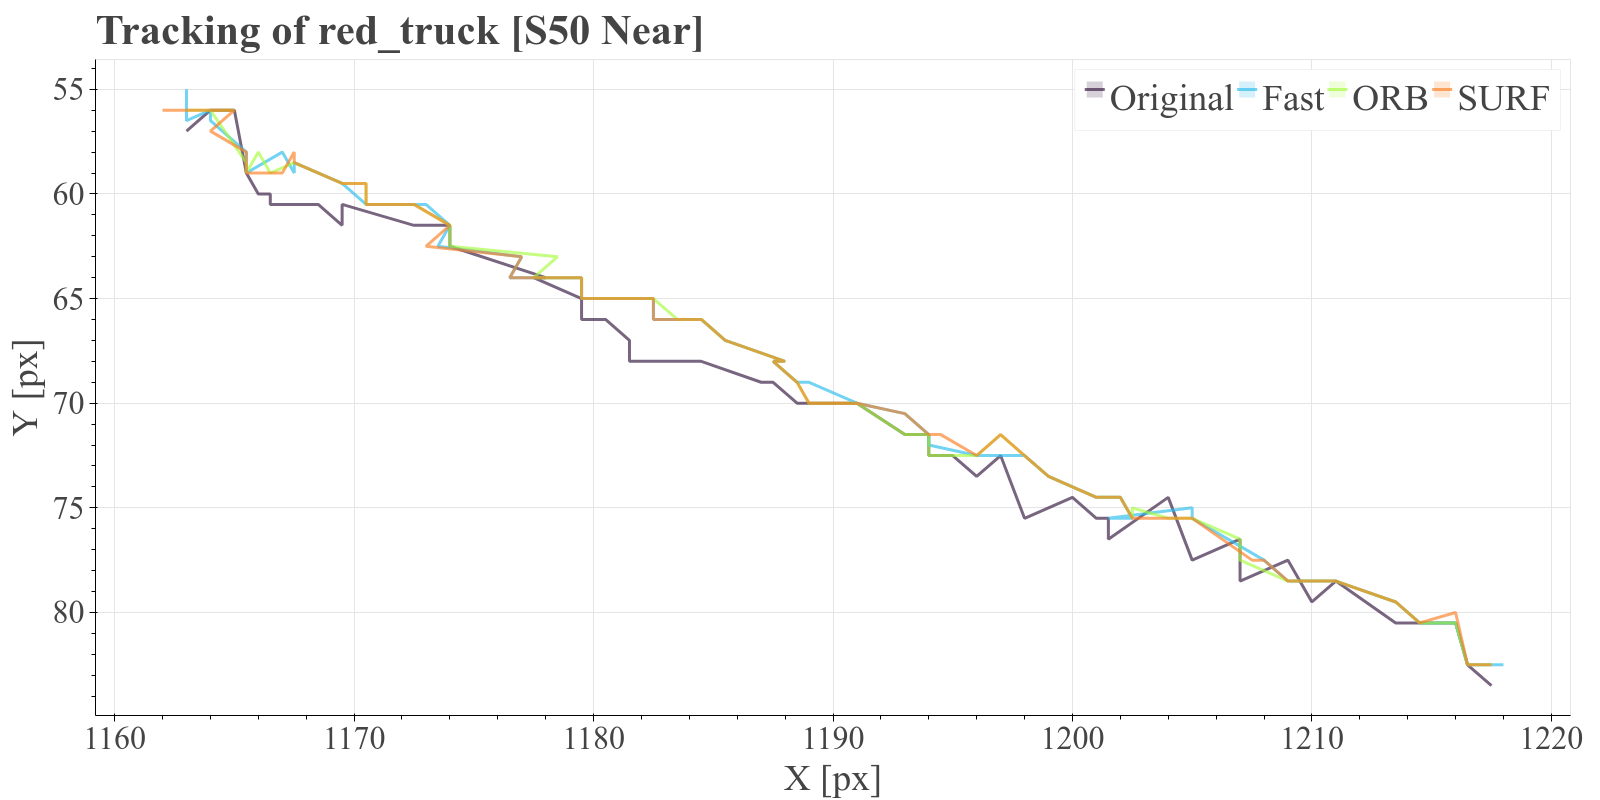
\includegraphics[width=0.475\linewidth]{diagrams/object_tracking/s50_s_near/red_truck.png}    &  
    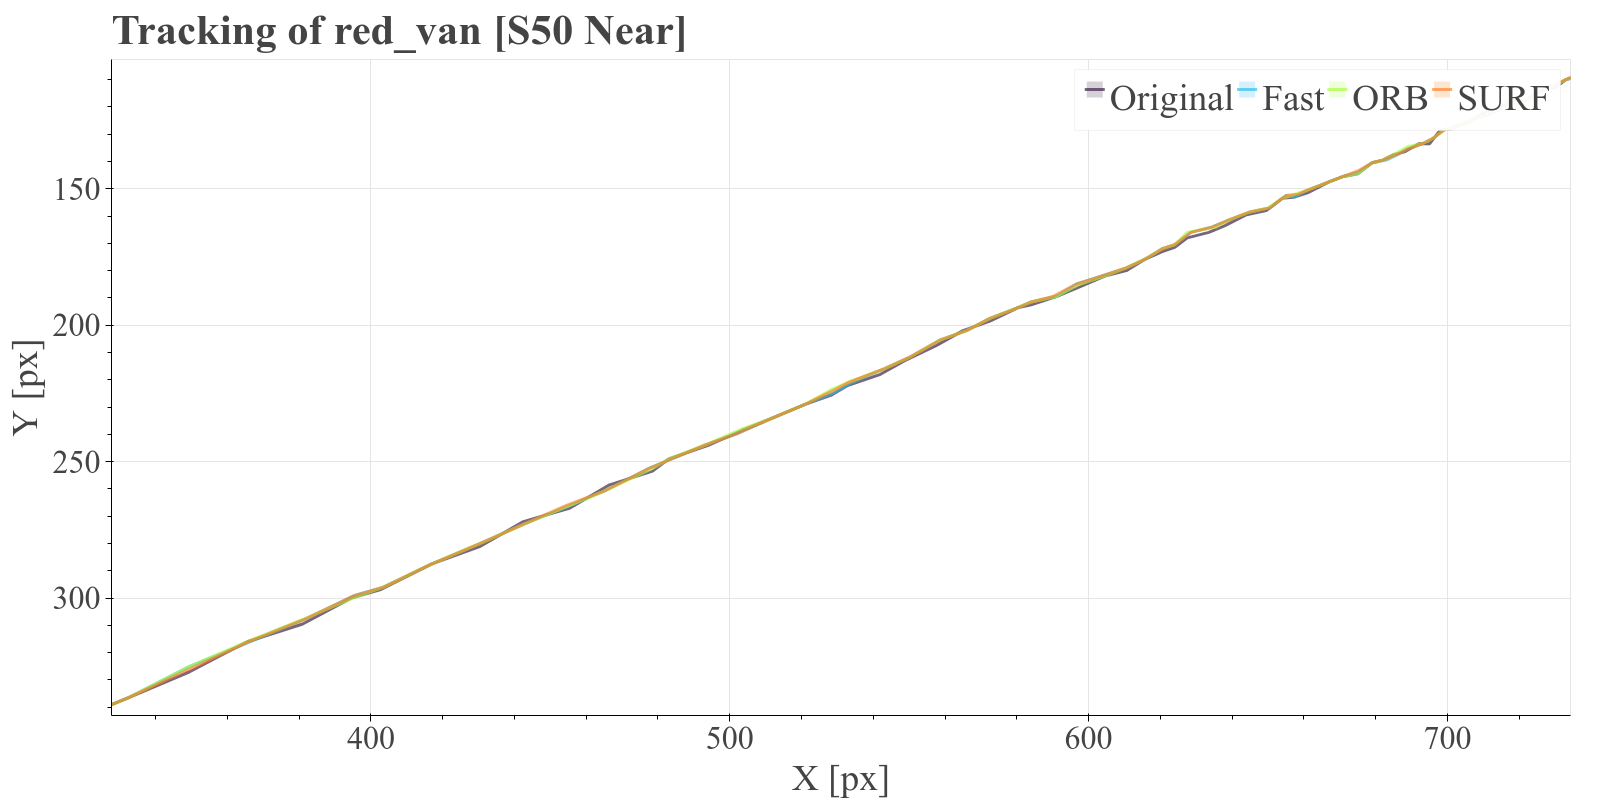
\includegraphics[width=0.475\linewidth]{diagrams/object_tracking/s50_s_near/red_van.png}    \\  
    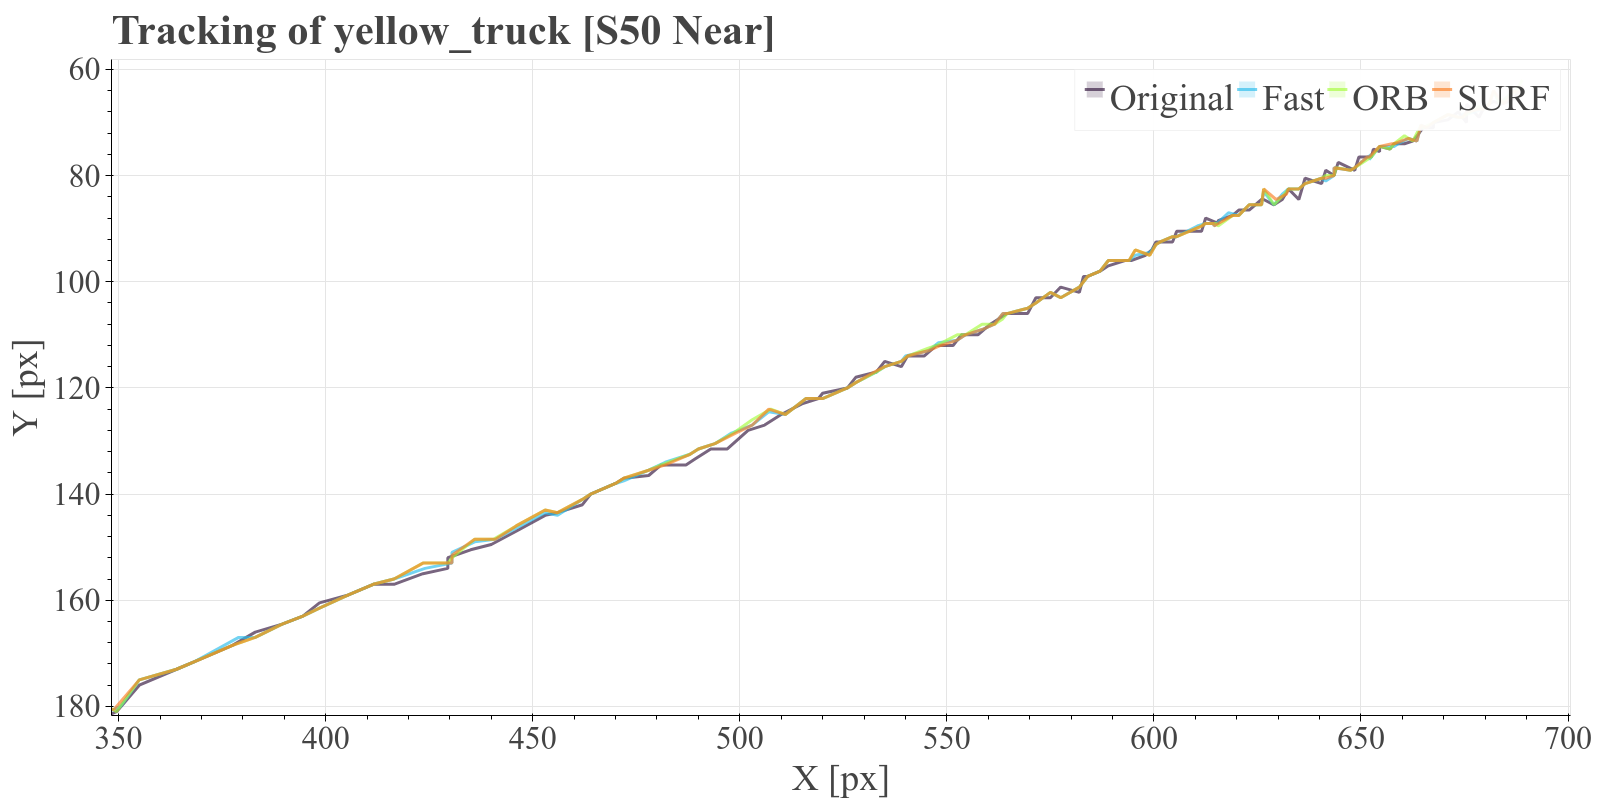
\includegraphics[width=0.475\linewidth]{diagrams/object_tracking/s50_s_near/yellow_truck.png}   
  \end{tabular}
  \caption{Left: 
  The exemplary vehicles tracked through the video sequence of the camera \camsn{4}. 
  Right:
  The corresponding normalized arc lengths of the pixel path. 
  The length is normalized by the original arc length, hence the 1.0 factor for the original video. 
  As the jitter is removed, the pixels movement is lowered significantly as it does only move with the vehicle, not the camera.
  This can be seen with around half of the path length remaining after stabilization for all stabilizers.
  }
  \label{fig:object_tracking_appendix_s50_s_near}
\end{figure*}




\end{document}
